\documentclass{article}
\usepackage[slovene]{babel}
\usepackage[a4paper, total={6in, 8in}]{geometry}
\usepackage[document]{ragged2e}
\usepackage{amsfonts}
\usepackage{amssymb}
\usepackage{amsmath}
\usepackage{amsthm}
\usepackage{tikz}
\usetikzlibrary{angles, quotes,babel}
\usepackage{float}
\usepackage{stmaryrd}
\usepackage{bbold}
\usepackage{tkz-euclide}
\usepackage{tzplot}
\usepackage{pgfplots}
\usepackage{cancel}
\usepackage{multicol}

\usepackage{hyperref}
\hypersetup{
    colorlinks,
    citecolor=black,
    filecolor=black,
    linkcolor=black,
    urlcolor=black
}

\usepackage{tocloft}

\cftsetindents{section}{0em}{2.5em}

\title{Vprašanja in odgovori za ustni izpit iz matematike na splošni maturi 2023 za višjo raven}

\date{Rožnik 2023}

\pgfplotsset{compat=1.18}
\begin{document}

\maketitle
Originalna \LaTeX datoteka je dostopna na \href{https://github.com/ChristofferNorgaard/Ustna-matura-iz-matematike-2023}{Githubu}.
\tableofcontents

\newpage
\section{Izjavni račun}
\subsubsection*{Kaj je izjava?}
Izjava je vsaka smiselna poved, ki ji lahko določimo logično vrednost (P – pravilna ali N – napačna). Izjave lahko zapisujemo tudi s simboli in jih označujemo z velikimi
črkami. Z izjavami lahko oblikujemo daljše ali sestavljene izjave. Pri rokovanju z izjavami uporabljamo logične operacije.

\subsubsection*{Kaj je negacija dane izjave? Kdaj je negacija pravilna (resnična) in kdaj nepravilna (neresnična)?}
NEGACIJA izjave je zanikanje dane izjave. Negacijo izjave A označimo z Ā ali ¬ A.
Če je A pravilna, je ¬ A nepravilna in obratno.

\subsubsection*{Kaj je konjunkcija izjav?}
KONKJUNKCIJA je vezava izjav z operacijo »in«. To je sestavljena izjava »A in B«, kar
označimo z $A \land B$. Konjunkcija izjav je pravilna le, če sta obe izjavi pravilni.
Če je A pravilna in B nepravilna, njuna konjunkcija ni pravilna. Če je A pravilna in B tudi, je
konjunkcija izjav A in B pravilna.

\subsubsection*{Kaj je disjunkcija izjav? Dokažite, da je izjava $\neg (A \land B)$ enakovredna izjavi $(\neg A) \lor (\neg B)$ za poljubni izjavi \emph{A} in \emph{B}.}

DISJUNKCIJA je vezava izjav z operacijo »ali«. To je sestavljena izjava »A ali B«, kar označimo z $A \lor B$. Disjunkcija izjav je pravila, čim je ena izmed izjav pravilna.
Če je A pravilna in B nepravilna, je njuna disjunkcija pravilna. Če je A nepravilna in B tudi, je
disjunkcija izjav nepravilna.

\begin{proof}
Izjavi $\neg (A \land B)$ in $(\neg A) \lor (\neg B)$ sta enakovredni za poljubni izjavi A in B. \\
\begin{table}[h!]
\begin{tabular}{cccccc}
{ \textbf{A}} & { \textbf{B}} & { \textbf{¬ A}} & { \textbf{¬ B}} & { \textbf{¬ (A ∧ B)}}        & { \textbf{(¬ A) ∨ (¬ B)}}    \\
{ P}          & { P}          & { N}            & { N}            & N & N \\
{ P}          & { N}          & { N}            & { P}            & P & P \\
{ N}          & { P}          & { P}            & { N}            & P & P \\
{ N}          & { N}          & { P}            & { P}            & P & P
\end{tabular}
\end{table}
Izjavi $\neg (A \land B)$ in $(\neg A) \lor (\neg B)$ sta enakovredni, saj sta njuni končni logični vrednosti enaki ne glede na začetni logični vrednosti A in B.

\end{proof}

\section{Izjavni račun}

\subsubsection*{Kaj je tavtologija? }
TAVTOLOGIJA je sestavljena izjava, ki je vedno pravilna.

\subsubsection*{Kaj je implikacija? Dokažite, da je izjava $A \Rightarrow B$ enakovredna izjavi $(\neg B) \Rightarrow (\neg A)$ za poljubni izjavi \emph{A} in \emph{B}.}

IMPLIKACIJA izjav je sestavljena izjava iz »A sledi B« oziroma »če A, potem B«, kar označimo $A \Rightarrow B$. Izjava A je pogoj/predpostavka, izjava B pa posledica. Implikacija izjav ni pravilna le, če iz pravilne izjave sklepamo na nepravilno

\begin{proof}
    Izjava $A \Rightarrow B$ je enakovredna izjavi $(\neg B) \Rightarrow (\neg A)$ za poljubni izjavi \emph{A} in \emph{B}.
    \begin{table}[h!]
\begin{tabular}{cccccc}
A & B & $A \Rightarrow B$ & $\neg B$ & $\neg A$ & $(\neg B) \Rightarrow (\neg A)$ \\
P & P & P     & N   & N   & P             \\
P & N & N     & P   & N   & N             \\
N & P & P     & N   & P   & P             \\
N & N & P     & P   & P   & P            
\end{tabular}
    \end{table}
    Izjava $A \Rightarrow B$ je enakovredna izjavi $(\neg B) \Rightarrow (\neg A)$, saj sta njuni končni logični vrednosti enaki ne glede na začetni logični vrednosti A in B.
\end{proof}

\subsubsection*{Kaj je ekvivalenca? Predstavite primer ekvivalence, ki je pravilna (resnična).}
    EKVIVALENCA izjav je sestavljena izjava »A natanko tedaj ko B« oziroma »A če in samo če B«, kar označimo A ⇔ B. Ekvivalenca izjav je pravilna, če imata izjavi enako logično vrednost.
Primer: ¬ (A ∧ B) je ekvivalentno ¬A ali ¬B.


\section{Množice}

\subsubsection*{Kaj je prazna množica in kaj je univerzalna množica? }
PRAZNA množica je množica brez elementov. Označimo jo \{ \} ali Ø.
UNIVERZALNA množica (U) je množica vseh elementov, ki nas v danem primeru
podrobneje zanimajo.

\subsubsection*{Kaj je razlika dveh množic? Kako označimo razliko dveh množic in kako jo grafično predstavimo? }
RAZLIKA množic A in B je množica vseh tistih elementov, ki so v množici A in niso v množici B. Označimo jo A – B ali A\textbackslash B.
\begin{figure}[H]
\begin{center}

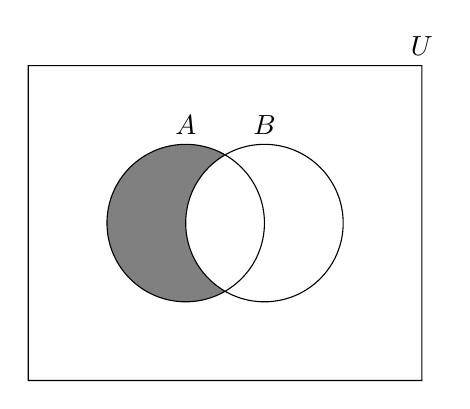
\begin{tikzpicture}[fill=gray]
% left hand
\scope
\clip (-2,-2) rectangle (2,2)
      (1,0) circle (1);
\fill (0,0) circle (1);
\endscope
% right hand
\scope
\clip (-2,-2) rectangle (2,2)
      (0,0) circle (1);
\endscope
% outline
\draw (0,0) circle (1) (0,1)  node [text=black,above] {$A$}
      (1,0) circle (1) (1,1)  node [text=black,above] {$B$}
      (-2,-2) rectangle (3,2) node [text=black,above] {$U$};
\end{tikzpicture}
\end{center}
\end{figure}
\subsubsection*{Kaj je komplement množice? }
KOMPLEMENT množice A je glede na univerzalno množico U je množica elementov, ki so v množici U in niso v množici A. Označimo jo $A^C$ ali $CA$.
\begin{figure}[H]
\begin{center}

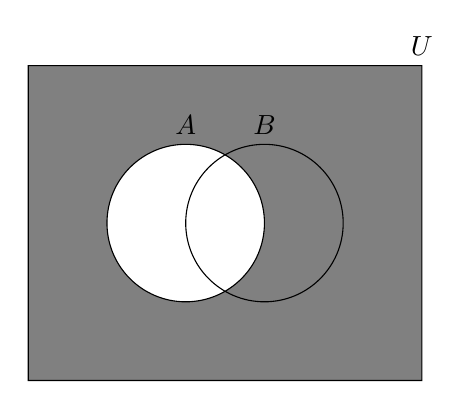
\begin{tikzpicture}[fill=gray]
% left hand
\scope

\clip (-2,-2) rectangle (2,2)
      (1,0) circle (1);
\endscope
% right hand
\scope
\clip (-2,-2) rectangle (2,2)
      (0,0) circle (1);
\fill (1,0) circle (1);
\fill (-2, -2) rectangle (2, 2);
\endscope
\fill (1, -2) rectangle (3, 2);
% outline
\draw (0,0) circle (1) (0,1)  node [text=black,above] {$A$}
      (1,0) circle (1) (1,1)  node [text=black,above] {$B$}
      (-2,-2) rectangle (3,2) node [text=black,above] {$U$};
      
\end{tikzpicture}
\end{center}
\end{figure}
\subsubsection*{Dokažite, da je $(A \cup B)^{c}=A^{c} \cap B^{c}$ za poljubni množici $A$ in $B$.}
\begin{proof}
    $(A \cup B)^C = A^C \cap B^C$ za poljubni množici $A$ in $B$.


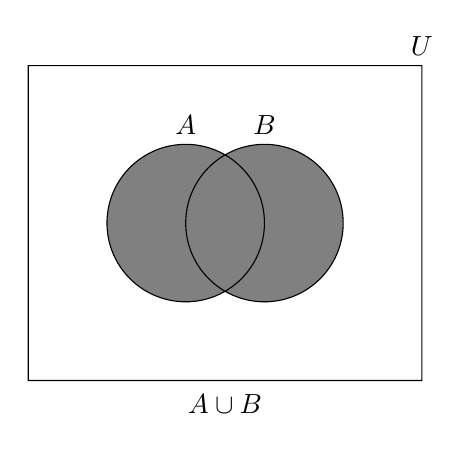
\begin{tikzpicture}[fill=gray]
% left hand
\scope
\fill (0,0) circle (1);
\endscope
% right hand
\scope
\fill (1,0) circle (1);
\endscope
% outline
\draw (0,0) circle (1) (0,1)  node [text=black,above] {$A$}
      (1,0) circle (1) (1,1)  node [text=black,above] {$B$}
      (-2,-2) rectangle (3,2) node [text=black,above] {$U$};
\node at (0.5, -2.3) {$A \cup B$};
\end{tikzpicture}
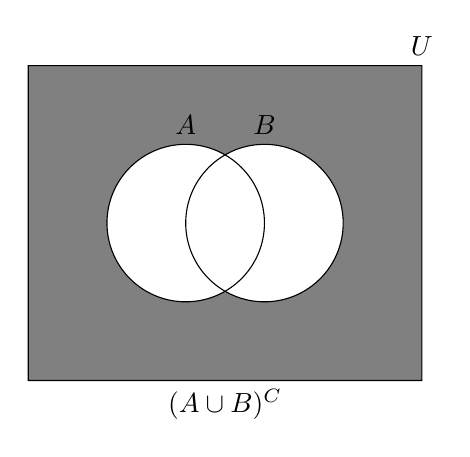
\begin{tikzpicture}[fill=gray]
% right hand
\scope
\clip (-2,-2) rectangle (3,2)
      (0,0) circle (1);
\clip (-2,-2) rectangle (3,2)
      (1,0) circle (1);
\fill (-2, -2) rectangle (3, 2);
\endscope
% outline
\draw (0,0) circle (1) (0,1)  node [text=black,above] {$A$}
      (1,0) circle (1) (1,1)  node [text=black,above] {$B$}
      (-2,-2) rectangle (3,2) node [text=black,above] {$U$};
\node at (0.5, -2.3) {$(A \cup B)^C$};
\end{tikzpicture}

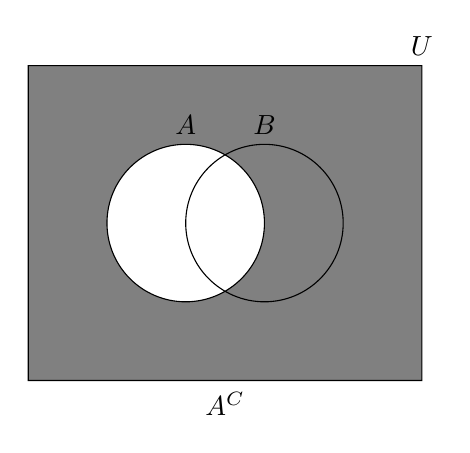
\begin{tikzpicture}[fill=gray]
% left hand
\scope

\clip (-2,-2) rectangle (2,2)
      (1,0) circle (1);
\endscope
% right hand
\scope
\clip (-2,-2) rectangle (2,2)
      (0,0) circle (1);
\fill (1,0) circle (1);
\fill (-2, -2) rectangle (2, 2);
\endscope
\fill (1, -2) rectangle (3, 2);
% outline
\draw (0,0) circle (1) (0,1)  node [text=black,above] {$A$}
      (1,0) circle (1) (1,1)  node [text=black,above] {$B$}
      (-2,-2) rectangle (3,2) node [text=black,above] {$U$};
\node at (0.5, -2.3) {$A^C$};
\end{tikzpicture}
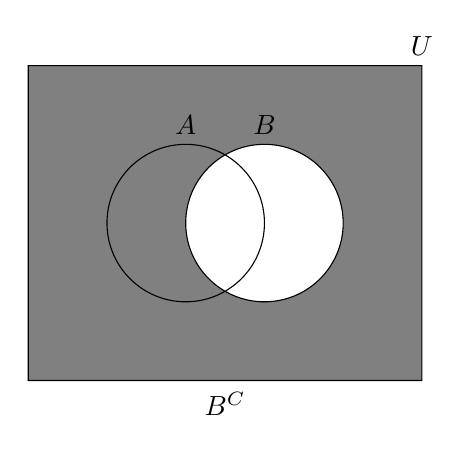
\begin{tikzpicture}[fill=gray]
% left hand
\scope

\clip (-2,-2) rectangle (2,2)
      (1,0) circle (1);
\endscope
% right hand
\scope
\clip (-2,-2) rectangle (3,2)
      (1,0) circle (1);
\fill (0,0) circle (1);
\fill (-2, -2) rectangle (3, 2);
\endscope
% outline
\draw (0,0) circle (1) (0,1)  node [text=black,above] {$A$}
      (1,0) circle (1) (1,1)  node [text=black,above] {$B$}
      (-2,-2) rectangle (3,2) node [text=black,above] {$U$};
\node at (0.5, -2.3) {$B^C$};
\end{tikzpicture}
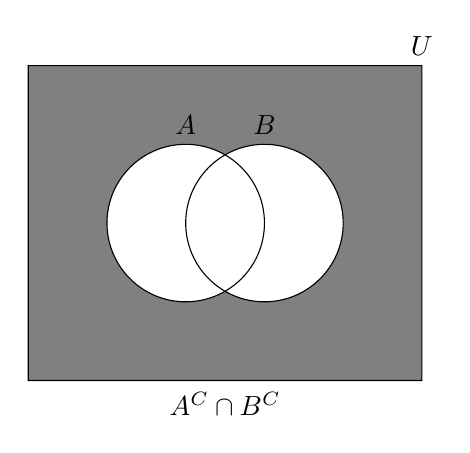
\begin{tikzpicture}[fill=gray]
% right hand
\scope
\clip (-2,-2) rectangle (3,2)
      (0,0) circle (1);
\clip (-2,-2) rectangle (3,2)
      (1,0) circle (1);
\fill (-2, -2) rectangle (3, 2);
\endscope
% outline
\draw (0,0) circle (1) (0,1)  node [text=black,above] {$A$}
      (1,0) circle (1) (1,1)  node [text=black,above] {$B$}
      (-2,-2) rectangle (3,2) node [text=black,above] {$U$};
\node at (0.5, -2.3) {$A^C \cap B^C$};
\end{tikzpicture}
\end{proof}


\section{Množice}
\subsubsection*{Kdaj je množica $A$ podmnožica množice $B$ ?}
Množica A je PODMNOŽICA množice B, če je vsak element množice A tudi element množice B. Označimo jo z $A \subseteq B$.



\subsubsection*{Kdaj sta dve množici enaki?}
Množici A in B sta ENAKI natanko tedaj, ko vsebujeta enake elemente. Označimo A = B.


\subsubsection*{Kaj je presek dveh množic? Moč množice $A$ je $n$, moč množice $B$ pa $m$. Ocenite, kolikšna je lahko moč množice $A \cap B$.}
PRESEK množic A in B je množica vseh tistih elementov, ki so v množici A in v množici B (lahko se ne sekata, lahko je ena podmnožica druge, lahko imata neprazen presek). Označimo $A \cap B$.

\begin{equation*}
    0 \le m(A \cap B) \le min(m, n)
\end{equation*}
Presek množic bo prazen, ko se množici ne sekata; presek bo neprazen, ko se množici delno prekrivata ali ko je ena podmnožica druge – v tem primeru bo presek enak množici, ki ima manj elementov.
Tem bolj se množici prekrivata, bolj bo njun presek enak manjši od množic.

\subsubsection*{Kaj je unija dveh množic? Moč množice $A$ je $n$, moč množice $B$ pa $m$. Ocenite, kolikšna je lahko moč množice $A \cup B$.}
UNIJA množic A in B je množica vseh tistih elementov, ki so v množici A ali v množici
B. Označimo $A \cup B$

\begin{equation*}
    max(m, n) \le m(A \cup B) \le m + n
\end{equation*}
Unija množic bo enaka množici z več elementi, ko je ena podmnožica druge; unija bo enaka vsoti elementov dveh množic, ko se množici ne sekata.
Tem bolj se množici prekrivata, bolj bo njuna unija enaka večji od množic.
\section{Naravna in cela števila}
\subsubsection*{Opišite množici $\mathbb{N}$ in $\mathbb{Z}$ in ju predstavite na številski premici.}

Naravna števila $\mathbb{N}$ so števila s katerimi štejemo (1, 2, 3, 4...). 1 je naravno število. Vsako naravno število ima naslednjika in vsak naslednjik naravnega števila je naravno število. V množici naravnih števil sta definirani operaciji seštevanje in množenje.

Cela števila $\mathbb{Z}$ dobim tako, da množici naravnih število dodamo še njihove nasprotne vrednosti in 0.
\begin{center}
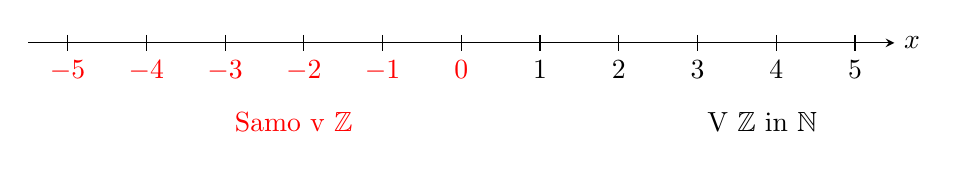
\begin{tikzpicture}
  % Number line
  \draw[->] (-5.5,0) -- (5.5,0) node[right] {$x$};

  % Natural numbers
  \foreach \x in {1,2,3,4,5} {
    \draw (\x,0.1) -- (\x,-0.1) node[below] {$\x$};
  }

  % Whole numbers
  \foreach \x in {0,-1,-2,-3,-4,-5} {
    \draw (\x,0.1) -- (\x,-0.1) node[red, below] {$\x$};
  }
  \draw(-3, -1) node[red, right] {Samo v $\mathbb{Z}$};
  \draw(3, -1) node[right] {V $\mathbb{Z}$ in $\mathbb{N}$};
\end{tikzpicture}
\end{center}
\subsubsection*{Navedite vsaj štiri lastnosti računskih operacij v množicah $\mathbb{N}$ in $\mathbb{Z}$.}

\begin{itemize}
\item $a + b = b + a$ 	komutativnostni zakon (za seštevanje)
\item $a + (b + c) = (a + b) + c$ 	asociativnostni zakon (za seštevanje)
\item $a + 0 = a$ 	zakon o nevtralnem elementu (za seštevanje)
\item $a + ( -a ) = 0$ 	zakon o inverznem (nasprotnem) elementu (za seštevanje)
\item $a b = b a$ 	komutativnostni zakon (za množenje)
\item $a (b c) = (a b) c$ 	asociativnostni zakon (za množenje)
\item $a 1 = a$ 	zakon o nevtralnem elementu (za množenje)
\item $a (b + c) = a b + a c$ 	distributivnostni zakon (za seštevanje in množenje) 
\end{itemize}
\subsubsection*{Kaj je matematična (popolna) indukcija? Razložite na primeru.}

Matematična indukcija je metoda za dokazovanje izjav, ki veljajo za vsa naravna števila ali naravna števila na intervalu.

Metoda matematične indukcije sestoji iz dveh korakov:

\begin{enumerate}
    \item Baza indukcije: Preverimo izjavo za začetno vrednost, običajno za $1$ ali $0$.
    \item Indukcijski korak: Predpostavimo, da izjava velja za neko naravno število $k$, nato pokažemo, da če izjava velja za $k$, potem velja tudi za $k+1$.
\end{enumerate}

Torej, če oba koraka uspešno izvedemo, potem lahko trdimo, da izjava velja za vsa naravna števila.

\textbf{Primer:}

Želimo dokazati, da je vsota prvih $n$ naravnih števil enaka $\frac{n(n+1)}{2}$ za vsako naravno število $n$.

\begin{proof}
  Uporabimo matematično indukcijo.

  \paragraph*{Baza indukcije:} 
  Za $n = 1$, izjava drži, saj je $1 = \frac{1(1+1)}{2}$.

  \paragraph*{Indukcijski korak:}
  Predpostavimo, da izjava drži za neko naravno število $k$. Torej,
  \[
  1 + 2 + 3 + \cdots + k = \frac{k(k+1)}{2}.
  \]
  Zdaj moramo pokazati, da če izjava velja za $k$, potem velja tudi za $k+1$. Enačbo ločimo na levo in desno stran. Leva stran je tako:
 \[
    L: \frac{k(k+1)}{2} + k + 1 = \frac{k^2 + k + 2k + 2}{2} = \frac{k^2 + 3k + 2}{2} = \frac{(k+1)(k+2)}{2}
 \]
    Nastavimo še desno stran, tako da v enačbo vstavimo $(k+1)$. Torej:
    \[
    D: \frac{(k+1)(k+1+1)}{2} = \frac{(k+1)(k+2)}{2}
    \]
    Velja $L=D$.
\end{proof}

Tako smo dokazali, da je izjava "vsota prvih $n$ naravnih števil je enaka $\frac{n(n+1)}{2}$" resnična za vsako naravno število $n$.

\section{Liha in soda števila}

\subsubsection*{Definirajte soda in liha števila.}

Celo število je SODO, če je deljivo z 2. Sodo število ima obliko $2k; \quad k \in \mathbb{Z}$.

Celo število je LIHO, če ni deljivo z 2. Liha števila imajo obliko $2k + 1; \quad k \in \mathbb{Z}$.

\subsubsection*{Pokažite, da je vsota dveh lihih števil sodo število.}

\begin{proof}
Vsota dveh lihih števil je sodo število.
Naj bosta $k$ in $m$ celi števili.
\begin{gather*}
    (2k + 1) + (2m + 1) = \\
    = 2k + 2m + 2 = \\
    = 2 (k + m + 1)
\end{gather*}
\end{proof}

\subsubsection*{Pokažite, da je kvadrat lihega števila liho število.}

\begin{proof}
Kvadrat lihega števila je liho število.
Naj bo $k$ celo število. 
\begin{gather*}
    (2k + 1)^2 = \\
    = 4k^2 + 4k + 1 = \\
    = 2 (2k^2 + 2k) + 1
\end{gather*}
\end{proof}

\subsubsection*{Pokažite, da je vsota dveh zaporednih lihih števil deljiva s 4.}

\begin{proof}
Vsota dveh zaporednih lihih števil je deljiva s 4.
Naj bo $k$ celo število. 
\begin{gather*}
    (2k - 1) + (2k + 1) = \\
    = 2k -1 + 2k +1 = \\
    = 4k
\end{gather*}
\end{proof}

\section{Praštevila}
\subsubsection*{Definirajte praštevilo in sestavljeno število. Naštejte tri praštevila in tri sestavljena števila.}
PRAŠTEVILO je vsako naravno število n > 1, ki ima natanko dva različna delitelja, 1 in n. Preštevil je neskončno mnogo. Vsako naravno število $n \neq 1$ je deljivo z vsaj enim praštevilom. To so na primer 2, 3, 5, 7, 11, 13, 17, 19 ...

SESTAVLJENO število je vsako naravno število, ki ima več kot dva delitelja.
To so števila 4, 6, 8, 9, 10, 12, 14, 15, 16, 18 ...

\subsubsection*{Kaj je razcep naravnega števila na prafaktorje? Ali je razcep na prafaktorje enoličen?}
RAZCEP števila na prafaktorje je zapis sestavljenega števila s produktom samih praštevil, kar je možno storiti na en sam način (če ne upoštevamo vrstnega reda faktorjev). Praštevilom v produktu pravimo prafaktorji.

\subsubsection*{Dokažite, da je praštevil neskončno mnogo.}
\begin{proof}
     Praštevil je neskončno mnogo.

Predpostavimo, da je praštevil končno, recimo n. Potem jih lahko po velikosti uredimo v končno zaporedje p1, p2, ... , pn. Sestavimo število P = p1 ·p2 ·...·pn +1 in poiščemo njegove delitelje. Seveda sta delitelja 1 in samo število P, toda drugih ni, saj P ni večkratnik nobenega od naših praštevil p1, p2, ... , pn. Zato je P praštevilo. Sestavili smo novo, večje praštevilo, kar je v nasprotju s predpostavko, da so praštevila le števila p1,p2,...,pn.

\end{proof}


\section{Deljivost}
\subsubsection*{Kdaj je naravno število $a$ večkratnik naravnega števila $b$?}
Naravno število a je večkratnik naravnega števila b, če obstaja tako naravno število k,
da velja a = b · k.
Število k je lahko tudi 1, v tem primeru je a = b, kar pomeni, da je to njegov najmanjši večkratnik.


\subsubsection*{Definirajte relacijo deljivosti množici $\mathbb{N}$.}

RELACIJA DELJIVOSTI: Naravno število a deli naravno število b, zapisano s simboli a|b, natanko takrat ko je število b večkratnik števila a.
Torej velja: $a | b \longleftrightarrow b = k \cdot a$ (ko je k naravno število)


Lastnosti deljivosti naravnih števil:
\begin{enumerate}
\item REFLEKSIVNOST
Vsako naravno število deli samo samega sebe.
\begin{equation*}
    a | a; a \in \mathbb{N}
\end{equation*}

\item ANTISIMETRIČNOST


Če za naravni števili a in b velja, da a deli b in b deli a, potem sta naravni števili a in b
enaki.

\begin{gather*}
    (a | b) \land (b | a) \Rightarrow a = b \\
    a, b \in \mathbb{N}
\end{gather*}

\item TRANZITIVNOST
Če naravno število a deli naravno število b in naravno število b deli naravno število c,
potem tudi a deli c.

\begin{gather*}
    (a | b) \land (b | c) \Rightarrow a | c \\
    a, b, c \in \mathbb{N}
\end{gather*}

\end{enumerate}

\subsubsection*{Opišite vsaj tri lastnosti relacije deljivosti.}

Lastnosti relacije deljivosti:

% TODO: A niso lastnosti relacije deljivosti refleksivnost, antisimetričnost pa tranzitivnost? (To kar je zgoraj) - popravljeno

\begin{enumerate}
    \item Refleksivnost
    \begin{equation*}
        a | a
    \end{equation*}

    \item Antisimetričnost
    \begin{equation*}
        a | b \land b | a \Rightarrow a = b
    \end{equation*}

    \item Tranzitivnost
    \begin{equation*}
        a | b \land b | c \Rightarrow a | c
    \end{equation*}

\end{enumerate}



\subsubsection*{Dokažite, da je relacija deljivosti tranzitivna.}
\begin{proof}
    Relacija deljivosti je tranzitivna. 
    \begin{gather*}
    (a | b) \land (b | c) \Rightarrow a | c \\
    a, b, c \in \mathbb{N}
    \end{gather*}
    Ker $a$ deli $b$, to pomeni, da je $b=ka$ za neko naravno število $k$. Ker $b$ deli $c$, to pomeni, da je $c=lb$ za neko naravno število $l$. Potem je $c = lb = lka$, torej je večkratnik števila $a$, zato velja a$|c$.

\begin{align*}
    a &| b \Rightarrow b=ka; k \in \mathbb{N} \\
    b &| c \Rightarrow c = lb; l \in \mathbb{N} \\
    c &= lb = lka \Rightarrow a | c
\end{align*}
% TODO: Tole bi se dal napisat z enačbami, kar je mogoče lepše, ampak drgač ok ... - Dodal sem enačbe poleg opisa.

\end{proof}


\section{Večkratniki in delitelji}
\subsubsection*{Definirajte največji skupni delitelj in najmanjši skupni večkratnik dveh naravnih števil. Razložite vsaj eno metodo za izračun najmanjšega skupnega večkratnika dveh naravnih števil.}

NAJVEČJI SKUPNI DELITELJ naravnih števil a in b je največje naravno število, ki deli števili a in b. Označimo D(a, b).

NAJMANJŠI SKUPNI VEČKRATNIK naravnih števil a in b je najmanjše število, ki je deljivo s številoma a in b. Označimo v(a, b).



Metoda za izračun najmanjšega skupnega večkratnika:
Števili razstavimo na prafaktorje. Najmanjši skupni večkratnik števil a in b je zmnožek vseh prafaktorjev iz razcepa a in b, za eksponent posameznega skupnega prafaktorja števil a in b izberemo največjega odobeh eksponentov.

PRIMER:
\begin{gather*}
    v(72, 90) = ? \quad D(72, 90) = ? \\
    72 = 3^2 \cdot 2^3 \\
    90 = 2 \cdot 3^2 \cdot 5 \\
    v(72, 90) = 2^3 \cdot 3^2 \cdot 5 = 360 \\
    D(72, 90) = 2 \cdot 3^2 = 18 \\
\end{gather*}

\subsubsection*{Povejte zvezo med $m, n, v(m, n)$ in $D(m, n)$.}
\begin{equation*}
    m \cdot n = v(m, n) \cdot D(m, n)
\end{equation*}


\subsubsection*{Kdaj sta si dve naravni števili tuji?}
Naravni števili sta si tuji, kadar je njun največji skupni delitelj 1.


\subsubsection*{Na primeru razložite Evklidov algoritem.}
Evklidov algoritem je postopek za računanje največjega skupnega delitelja D(a, b) dveh števil a in b brez razcepa števil na prafaktorje. Algoritem temelji na osnovnem izreku o deljenju
$b = k \cdot a + r; (b > a, 0 r < a)$, in ugotovitvi, da je $D(a, b) = D(a, r)$. Postopke vključuje več zpaorednih verižnih deljenj in je končan, ko se deljenje izide.
Največji skupni delitelj števil a in b je zadnji od 0 različni ostanek, ki ga dobimo v Evklidovem algoritmu.

PRIMER: 
\begin{gather*}
    D(448, 372) = ? \\
    448 = 1 \cdot 378 + 70 \\
    378 = 5 \cdot 70 + 28 \\
    70 = 2 \cdot 28 + 14 \\
    28 = 2 \cdot 14 + 0 \\
    D(448, 378) = D(378, 70) = D(70, 28) = D(28, 14) = 14 \\
\end{gather*}

\section{Deljenje naravnih števil}
\subsubsection*{Povejte osnovni izrek o deljenju naravnih števil.}
$\text{Za poljubni dve števili } n \text{ in } m \text{ (} n \geq m \text{) obstajata točni taki enolično določeni števili } k \text{ in } r \text{ (} k > 0 \text{ in } 0 \leq r < m \text{)}, \text{ da velja } n = k \cdot m + r.$

\subsubsection*{Koliko je ostanek pri deljenju naravnega števila $n$ z naravnim številom $m$, če je število $n$ večkratnik števila $m$ ?}
Če je naravno število n večkratnik naravnega števila m, je ostanek pri deljenju števila n s številom m enak 0.


\subsubsection*{Naj bo $k$ naravno število. Opišite množico vseh ostankov pri deljenju z naravnim številom $k$.}
Pri deljenju z naravnim številom $k$ bo ostanek $r$ imel vrednost $0 \leq r < k$. 


\section{Kriteriji deljivosti}
\subsubsection*{Za vsako število $k \in\{2,3,4,5,6,8,9,10\}$ navedite kriterij deljivosti s številom $k$.}
\begin{itemize}
\item \textbf{2}: na zadnjem mestu je števka 0, 2, 4, 6 ali 8
\item \textbf{3}: vsota števk je deljiva s 3
\item \textbf{4}: število, sestavljeno iz zadnjih dveh števk števila, je deljivo s 4
\item \textbf{5}: na zadnjem mestu je števka 0 ali 5
\item \textbf{6}: število je deljivo z 2 in 3 hkrati
\item \textbf{8}: število, sestavljeno iz zadnjih treh števk števila, je deljivo z 8
\item \textbf{9}: vsota števk je deljiva z 9
\item \textbf{10}: na zadnjem mestu je števka 0
\end{itemize}
\subsubsection*{Izpeljite kriterij deljivosti s številom 2.}

Naj bo \( a_{n-1}a_{n-2} \ldots a_2a_1a_0 \) desetiški zapis števila \( a \) (\( a_1, a_2, \ldots, a_n \) so števke števila).
Tedaj je
\[
a = a_n \cdot 10^n + a_{n-1} \cdot 10^{n-1} + \ldots + a_2 \cdot 10^2 + a_1 \cdot 10^1 + a_0 
\]
in
\[
a = 10 \cdot (a_n \cdot 10^{n-1} + a_{n-1} \cdot 10^{n-2} + \ldots + a_2 \cdot 10^1 + a_1 ) + a_0 
\]
in
\[
a = 2 \cdot 5 \cdot (a_n \cdot 10^{n-1} + a_{n-1} \cdot 10^{n-2} + \ldots + a_2 \cdot 10^1 + a_1 ) + a_0
\]
Prvi člen vsote je deljiv z 2, zato mora biti tudi $a_0$ deljiv z 2, če hočemo, da bo število deljivo z dve.
\section{Ulomki in racionalna števila}
\subsubsection*{Kaj je ulomek? Kdaj dva ulomka predstavljata isto racionalno število?}
ULOMEK je izraz oblike $\frac{a}{b}$  kjer sta a in b celi števili in $b \neq 0$. Število a je števec ulomka $\frac{a}{b}$ in število $b$ imenovalec ulomka. Ulomek $\frac{a}{b}$ lahko zapištemo v obliki $a \cdot b^-1$. 

RACIONALNO ŠTEVILO je število, ki ga lahko predstavimo z ulomkom oblike $\frac{a}{b}$ , kjer sta a in b celi števili in b različen od 0. Ulomka $\frac{a}{b}$ in $\frac{c}{d}$ predstavljata isto racionalno število natanko takrat, ko je zmnožek števca prvega ulomka in imenovalca drugega ulomka enak zmnožku števca drugega ulomka in imenovalca prvega ulomka.
\begin{equation*}
    \frac{a}{b} = \frac{c}{d} \Leftrightarrow a \cdot d = b \cdot c
\end{equation*}
\subsubsection*{Kako je definirana relacija $\leq$ v množici $\mathbb{Q}$ ? Opišite vsaj dve lastnosti te relacije.}

Množica racionalnih števil $\mathbb{Q}$ je urejena z relacijo »manjši ali enak« in jo označimo $\leq$. Za poljubni racionalni števili $\frac{a}{b}$ in $\frac{c}{d}$ velja: $\frac{a}{b}>\frac{c}{d}$ ali $\frac{a}{b}<\frac{c}{d}$ ali $\frac{a}{b}=\frac{c}{d}$.

Racionalno število $\frac{a}{b}$ je pozitivno $\left(\frac{a}{b}>0\right)$, če sta a in b enako predznačena, negativno $\left(\frac{a}{b}<0\right)$, če sta a in b različno prednzačena, in enako 0, če je $a=0$. Množica racionalnih števil $\mathbb{Q}$ je unija treh disjunktnih (tujih si) množic $\mathbb{Q}^{-},\{0\}$ in $\mathbb{Q}^{+}$.

Lastnosti relacije: Naj bodo $p, q$ in $r$ racionalna števila. Potem velja:
\begin{itemize}
\item REFLEKSIVNOST: $p \leq p$ za vaka racionalno število $p$
\item ANTISIMETRIČNOST: Če je $p \leq q$ in $q \leq p$, potem je $q=p$.
\item TRANZITIVNOST: Če je $p \leq q$ in $q \leq r$, potem je tudi $p \leq r$.
\end{itemize}

\subsubsection*{Pokažite, da za poljubni racionalni števili $p$ in $q$, kjer je $p<q$, obstaja tako racionalno število $r$, da je $p<r<q$.}
\begin{proof}
    Med poljubnima racionalnima številoma leži vsaj še eno racionalno število.

    Naj bosta a in b racionalni števili ter $a<b$. Pokažimo, da število $\frac{a+b}{2}$ leži med številoma $a$ in $b$, torej $a<\frac{a+b}{2}<b$. Ker je $a<b$, je razlika $\frac{a+b}{2}-a=\frac{b-a}{2}$ pozitivno število, kar pomeni, da je $a<\frac{a+b}{2}$. Prav tako je razlika $b-\frac{a+b}{2}=\frac{b-a}{2}$ pozitivno število, kar pomeni, da je $\frac{a+b}{2}<b$. Iz tega sledi, da je $a<\frac{a+b}{2}<b$.
\end{proof}

\section{Ulomki in decimalni zapis}
\subsubsection*{Kako iz decimalnega zapisa števila prepoznamo, da lahko to število zapišemo z ulomkom? Kako poljubnemu ulomku priredimo njegov decimalni zapis? Kako iz zapisa ulomka ugotovimo, ali ima končen decimalni zapis?}

\begin{itemize}
  \item Če je decimalni zapis številke končen ali pa neskončen periodičen, gre za racionalno številko, ki jo lahko zapišemo z ulomkom.
\end{itemize}

Poljubnemu ulomku priredimo njegov decimalni zapis z običajnim deljenjem števca z imenovalcem. Računanje se preneha po končnem številu korakov ali pa teče brez konca - števke ali skupina števk se od nekod naprej začnejo ponavljati. Med obema možnostima odloča imenovalec b, če je ulomek do konca okrajšan.

Iz zapisa ulomka ugotovimo, ali ima končen decimalni zapis tako, da preverimo, ali ima ulomek imenovalec oblike $\mathbf{2}^{\mathrm{m}} \cdot \mathbf{5}^{\mathrm{n}}$ (kjer sta $\mathrm{m}$ in $\mathrm{n}$ naravni števili) - sicer je decimalni zapis neskončen. (Končen decimalni zapis imajo desetiški ulomki, torej tisti, ki imajo imenovalec, ki je potenca števila 10 oziroma se jih da razširiti na take ulomke.)

\subsubsection*{Podajte primer ulomka, ki ima končen decimalni zapis, in primer ulomka, ki ima neskončen decimalni zapis.}

Ulomek, ki ima končen decimalni zapis: $\frac{4}{5}=0,8$

Ulomek, ki ima neskončen decimalni zapis: $\frac{5}{11}=0,45454545 \ldots$

\subsubsection*{Podajte primer periodičnega decimalnega števila s periodo reda (dolžine) vsaj 2 in ga zapišite kot ulomek.}

PRIMER periodičnega decimalnega števila s periodo reda vsaj 2: $\frac{2}{11}=0,181818 \ldots$

\begin{gather*}
    x=0,181818 \\
    100 x=18,1818 \\
    100 x-x=99 x \\
    99 x=18 \\
    x=\frac{18}{99}=\frac{2}{11} \\
\end{gather*}


\section{Realna števila}
\subsubsection*{Kdaj je realno število racionalno in kdaj iracionalno? Kako se razlikujeta njuna decimalna zapisa?}

Racionalna števila so števila, ki jih lahko zapišemo z ulomki oblike $\frac{a}{b}$, kjer sta a in b celi števili in b ni enak nič. Ostala realna števila so iracionalna. Decimalni zapisi racionalnih števil so ali končni ali pa imajo periodo. Iracionalna števila v decimalnem zapisu niso končna in nimajo periode.

\subsubsection*{Naštejte vsaj tri primere racionalnih števil in vsaj tri primere iracionalnih števil}

Racionalna števila: $3, \frac{5}{11}, \frac{1}{4}$

Iracionalna števila: $e, \boldsymbol{\pi}, \sqrt{\mathbf{3}}$

\subsubsection*{Dokažite, da $\sqrt{2}$ ni racionalno število.}
\begin{proof}
    $\sqrt{2}$ ni racionalno število.

    Recimo, da je število $\sqrt{2}$ racionalno, potem se ga da zapisati kot okrajšan ulomek oblike: $\sqrt{2}=\frac{a}{b}$. Po kvadriranju dobimo $2=\frac{a^{2}}{b^{2}}$, od koder sklepamo $a^{2}=2 \mathrm{~b}^{2}$. To pomeni, da je $a^{2}$ sodo in je tudi a sodo število, zato ga lahko zapišemo kot večkratnik števila 2, torej $a=2 \mathrm{k}$. Če to vstavimo $v a^{2}=2 \mathrm{~b}^{2}$, dobimo $4 \mathrm{k}^{2}=2 \mathrm{~b}^{2}$ in $b^{2}=2 \mathrm{k}^{2}$, kar pomeni, da je $b^{2}$ sodo število in s tem tudi b sodo število. Prišli smo v nasprotje s trditvijo, da sta si a in $b$ tuji si števili. Števili $a$ in $b$ ne moreta biti obe sodi. Zato $\sqrt{2}$ ne more biti racionalno število.
\end{proof}


\section{\texorpdfstring{\cancel{Absolutna vrednost}}{Absolutna vrednost}}
\subsubsection*{Definirajte absolutno vrednost realnega števila in razložite njen geometrijski pomen.}

Absolutna vrednost realnega števila je enočlena operacija, ki pozitivna števila in 0 ohranja, negativnim številom pa spreminja predznak.
$$
|a| =     \begin{cases}
      a, & a \geq 0 \\
      -1, & a < 0
    \end{cases}
$$

$|a|$ grafično pomeni oddaljenost točke $a$ od izhodišča številske premice.

\subsubsection*{Navedite vsaj štiri lastnosti absolutne vrednosti realnega števila.}

\begin{enumerate}
    \item $|a| = |-a|$ recimo $|3| = |-3|$
    \item $|a| \geq 0 \land |a| = 0 \Leftrightarrow a = 0$ recimo $|-3| = 3$
    \item $|a| \cdot |b| = |a \cdot b|$ recimo $|-2| \cdot |-3| = |-2 \cdot -3|$
    \item $|a + b| \leq |a| + |b|$ recimo $|-2 + 3| \leq |-2| + |3|$
\end{enumerate}

\subsubsection*{Dokažite, da za poljubni realni števili $x$ in $y$ velja $|x+y| \leq|x|+|y|$.}

\begin{proof}
    $|x+y| \leq |x| + |y| \Rightarrow |x| + |y| - |x+y| \geq 0$
    \begin{enumerate}
        \item Recimo da je $x \geq 0 \land y \geq 0$ \\
        Potem $|x| + |y| - |x+y| \geq 0 \Rightarrow x + y - x - y = 0$
        \item Recimo da je $x < 0 \land y < 0$ \\
        Potem $|x| + |y| - |x+y| \geq 0 \Rightarrow -x -y +x + y = 0$
        \item Recimo da je $x+y \geq 0 \land y < 0$ \\
        Potem $|x| + |y| - |x+y| \geq 0 \Rightarrow x -y - x - y = -2y$ ampak $y < 0$ torej $-2y > 0$
        \item Recimo da je $x+y < 0 \land y < 0$ \\
        Potem $|x| + |y| - |x+y| \geq 0 \Rightarrow x -y + x + y = 2x > 0$ ker $x > 0$
    \end{enumerate}
    Zaradi komutativnost lahko pri primeru 3 in 4 $x$ in $y$ brez težav zamenjamo tako da bi bil $x < 0$ in $y \geq 0$. 
\end{proof}

\section{Kompleksna števila}
\subsubsection*{Definirajte množico kompleksnih števil.}

Množico realnih števil R razširimo na množico kompleksnih števil $\mathbb{C}$, kjer je rešljiva vsaka polinomska enačba. Primer je $x^{\mathbf{2}}=-\mathbf{1}$, ki nima realnih rešitev enačb (saj kvadrat realnega števila ne more biti negativen). 

Kompleksno število $z$ določa urejen par realnih števil $(a, b)$ in ga zapišemo v obliki $z=a+\mathbf{b i}$. Število a je realna komponenta in število $b$ imaginarna komponenta kompleksnega števila z. Število $i$ je imaginarna enota za katero velja: $\mathrm{i}^{2}=-1 . \mathrm{V}$ množici kompleksnih števil so realna števila predstavljena z urejenimi pari $(a, 0)$. Kompleksna števila, ki jih zapišemo s pari $(0, b)$, imenujemo čista imaginarna števila.

\subsubsection*{Kako grafično upodobimo (predstavimo) kompleksna števila?}

Množico kompleksnih števil $\mathbb{C}$ lahko upodobimo z množico vseh točk na kompleksni ravnini, kjer je $x$ os realna os Re in $y$ os imaginarna os Im (nariši primer enega kompleksnega števila v ravnini!)
\begin{center}
\begin{tikzpicture}
    % Draw axes
    \draw[->] (-0.5,0) -- (4,0) node[right] {$Re$};
    \draw[->] (0,-0.5) -- (0,4) node[above] {$Im$};

    % Label x-axis ticks
    \foreach \x in {1,2,3}
        \draw (\x,0.1) -- (\x,-0.1);

    % Label y-axis ticks
    \foreach \y in {1,2,3}
        \draw (0.1,\y) -- (-0.1,\y);

    \draw (2,0.1) -- (2,-0.1) node[below] {$a$};
    \draw (0.1,3) -- (-0.1,3) node[left] {$b$};
    \draw[gray, dashed] (2, 0) -- (2, 3);
    \draw[gray, dashed] (0, 3) -- (2, 3);
    \draw[->] (0,0) -- (2,3);

    % Draw a point at (2,3)
    \fill (2,3) circle[radius=2pt] node[above right] {$z=a+bi$};
\end{tikzpicture}
\end{center}

\subsubsection*{Definirajte seštevanje kompleksnih števil.}
Seštevanje kompleksnih števil: kompleksni števili seštejemo tako, da seštejemo njuna realna in njuna imaginarna dela.
\begin{equation*}
    z_{1}+z_{2}=(a+b i)+(c+d i)=(a+c)+(b+d) i
\end{equation*}


\subsubsection*{Navedite eno lastnost seštevanja kompleksnih števil in jo dokažite.}
KOMUTATIVNOST $z_{1}+z_{2}=z_{2}+z_{1}$:
\begin{proof}
    Komutativnosti pri seštevanju kompleksnih števil.
    $\mathrm{z}_{1}=a+\mathrm{bi}, \mathrm{z}_{2}=\mathrm{c}+\mathrm{di}$

$z_{1}+z_{2}=(a+c)+(b+d) i-p o$ definiciji seštevanja, navedeni zgoraj

$a, b, c$ in d so realna števila, za seštevanje realnih števil pa velja komutativnost, torej je $a+c=c+a$ in $b+d=d+b$. Potem je $z_{1}+z_{2}=(a+c)+(b+d) i=(c+a)+(d+b) i=z_{2}+z_{1}$
\end{proof}
 

\subsubsection*{Kakšen geometrijski pomen ima seštevanje kompleksnih števil?}

\begin{center}
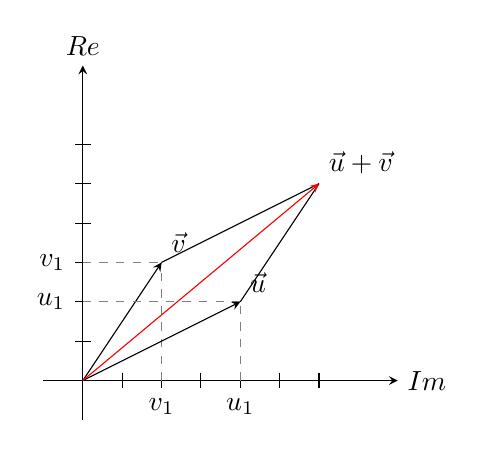
\begin{tikzpicture}
    % Draw axes
    \draw[->] (-0.5,0) -- (4,0) node[right] {$Im$};
    \draw[->] (0,-0.5) -- (0,4) node[above] {$Re$};

    % Label x-axis ticks
    \foreach \x in {0.5,1, 1.5, 2, 2.5, 3}
        \draw (\x,0.1) -- (\x,-0.1);

    % Label y-axis ticks
    \foreach \y in {0.5,1, 1.5, 2, 2.5, 3}
        \draw (0.1,\y) -- (-0.1,\y);

    \draw (1,0.1) -- (1,-0.1) node[below] {$v_1$};
    \draw (0.1,1.5) -- (-0.1,1.5) node[left] {$v_1$};
    \draw[gray, dashed] (1, 0) -- (1, 1.5);
    \draw[gray, dashed] (0, 1.5) -- (1, 1.5);
    \draw[->] (0,0) -- (1,1.5);

    \fill (1,1.5) node[above right] {$\vec{v}$};

    \draw (2,0.1) -- (2,-0.1) node[below] {$u_1$};
    \draw (0.1,1) -- (-0.1,1) node[left] {$u_1$};
    \draw[gray, dashed] (2, 0) -- (2,1);
    \draw[gray, dashed] (0, 1) -- (2,1);
    \draw[->] (0,0) -- (2,1);

    \fill (2,1) node[above right] {$\vec{u}$};
    \draw[-] (2,1) -- (3, 2.5);
    \draw[-] (1, 1.5) -- (3, 2.5);

    \fill (3,2.5) node[above right] {$\vec{u} + \vec{v}$};
    \draw[->, red] (0, 0) -- (3, 2.5);
\end{tikzpicture}
\end{center}

Vsako kompleksno število v kompleksni ravnini lahko predstavimo z vektorjem, ki poteka od koordinatnega izhodišča do točke, ki predstavlja kompleksno število. Vsoti kompleksnih števil $z_{1}$ in $z_{2}$ ustreza vsota vektorjev, ki pripadata kompleksnima številoma $z_{1}$ in $z_{2}$.


\section{Množenje kompleksnih števil}
\subsubsection*{Definirajte operacijo množenja v množici $\mathbb{C}$.}

Če sta $z_{1}=a+b i$ in $z_{2}=c+d i$, potem dobimo njun produkt tako, da pomnožimo vsak člen z vsakim in upoštevamo, da je $\mathrm{i}^{2}=-1$. Torej:
\begin{equation*}
    z_{1} \cdot z_{2}=(a+b i) \cdot(c+d i)=(a c-b d)+(a d+b c) i
\end{equation*}

\subsubsection*{Opišite geometrijski pomen množenja kompleksnega števila z -1 in geometrijski pomen množenja kompleksnega števila z realnim številom.}

Kompleksno štveilo $-\mathrm{z}=(-1) z$ je tisto število, ki ga določa nasprotni vektor vektorja, ki določa kompleksno število z.

Kompleksno število $k \cdot z$, kjer je $k$ realno število, je tisto število, ki je določeno $z$ večkratnikom vektorja, ki določa število z.

\subsubsection*{Naštejte vsaj dve lastnosti množenja kompleksnih števil in vsaj eno od njih dokažite.}

KOMUTATIVNOST:
\begin{equation*}
z_{1} \cdot z_{2}=z_{2} \cdot z_{1}
\end{equation*}

ASOCIATIVNOST:
\begin{equation*}
\left(z_{1} \cdot z_{2}\right) \cdot z_{3}=z_{1} \cdot\left(z_{2}+z_{3}\right)
\end{equation*}

\begin{proof}
    Komutativnosti pri množenju kompleksnih števil:
    $\mathrm{z}_{1}=a+\mathrm{bi}, \mathrm{z}_{2}=\mathrm{c}+\mathrm{di}$

$z_{1} \cdot z_{2}=(a+b i) \cdot(c+d i)=(a c-b d)+(a d+b c) i=(c a-d b)+(d a+c b) i-p o$ definiciji

komutativnosti množenja realnih števil, navedeni zgoraj

$=(c a-d b)+(c b+d a) i-$ po definiciji komutativnosti seštevanja realnih števil

$=\mathrm{z}_{2} \cdot \mathrm{z}_{1}$
\end{proof}
\subsubsection*{Naj bo $n$ naravno število. Izračunajte $i^{n}$.}

$\mathrm{i}^{\mathrm{n}}=1$, če je $\mathrm{n}$ večkratnik števila 4 ;

$\mathrm{i}^{\mathrm{n}}=\mathrm{i}$, če da n pri deljenju s 4 ostanek 1 ;

$\mathrm{i}^{\mathrm{n}}=-1$, če da $\mathrm{n}$ pri deljenju s 4 ostanek 2 ;

$\mathrm{i}^{\mathrm{n}}=-\mathrm{i}$, če da $\mathrm{n}$ pri deljenju s 4 ostanek 3

\section{Absolutna vrednost kompleksnega števila}
\subsubsection*{Definirajte absolutno vrednost kompleksnega števila in predstavite njen geometrijski pomen.}
Absolutna vrednost kompleksnega števila $z=a+$ bi je nenegativno realno število, določeno s predpisom
\begin{equation*}
    |z|=\sqrt{z \cdot \bar{z}}=\sqrt{(a+b i)(a-b i)}=\sqrt{a^{2}+b^{2}}
\end{equation*}

V kompleksni ravnini je absolutna vrednost kompleksnega števila enaka razdalji točke (a, b) od izhodišča.

\begin{center}
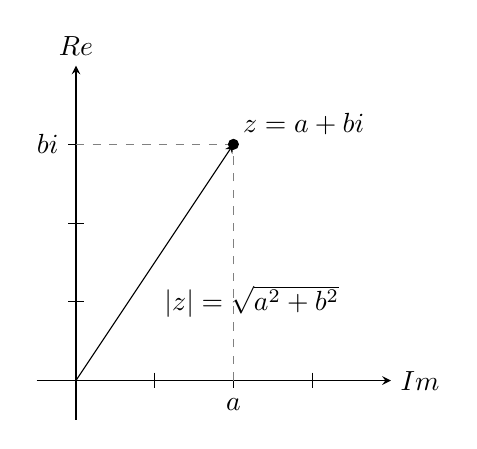
\begin{tikzpicture}
    % Draw axes
    \draw[->] (-0.5,0) -- (4,0) node[right] {$Im$};
    \draw[->] (0,-0.5) -- (0,4) node[above] {$Re$};

    % Label x-axis ticks
    \foreach \x in {1,2,3}
        \draw (\x,0.1) -- (\x,-0.1);

    % Label y-axis ticks
    \foreach \y in {1,2,3}
        \draw (0.1,\y) -- (-0.1,\y);

    \draw (2,0.1) -- (2,-0.1) node[below] {$a$};
    \draw (0.1,3) -- (-0.1,3) node[left] {$bi$};
    \draw[gray, dashed] (2, 0) -- (2, 3);
    \draw[gray, dashed] (0, 3) -- (2, 3);
    \draw[->] (0,0) -- (2,3);

    % Draw a point at (2,3)
    \fill (2,3) circle[radius=2pt] node[above right] {$z=a+bi$};
    \path (1,1) node[right] {$|z| = \sqrt{a^2 + b^2}$};
\end{tikzpicture}
\end{center}

\subsubsection*{Naštejte vsaj dve lastnosti absolutne vrednosti kompleksnega števila in vsaj eno od njih dokažite.}

\begin{enumerate}
  \item $\left|z_{1} \cdot z_{2}\right|=\left|z_{1}\right|\left|z_{2}\right|$

  \item $|-z|=|z|$

  \item $|z|=|\bar{z}|$

  \item $\left|\frac{z_{1}}{z_{2}}\right|=\frac{\left|z_{1}\right|}{\left|z_{2}\right|} ; z_{2} \neq 0$

  \item $\left|z_{1}+z_{2}\right| \leq\left|z_{1}\right|+\left|z_{2}\right|$

\end{enumerate}

\begin{proof}
    $|z|=|\bar{Z}|$
    \begin{gather*}
        z=x+y i \\
        \bar{z}=x-y i \\
        |z|=|\overline{\mathrm{z}}|=\sqrt{\mathrm{z} \cdot \overline{\mathrm{z}}}=\sqrt{\overline{\overline{\mathrm{z}} \cdot \overline{\mathrm{z}}}}=\sqrt{x^{2}+y^{2}}
    \end{gather*}
\end{proof}
\subsubsection*{Pojasnite absolutno vrednost kompleksnega števila $z$, če je $\operatorname{Im}(z)=0$ ali $\operatorname{Re}(z)=0$.} 
\begin{itemize}
  \item Če je $\operatorname{Im}(z)=0$, potem je $z=a+b i=a$ in je njegova absolutna vrednost $|z|=|a|$.
  \item Če je $\operatorname{Re}(z)=0$, potem je $z=a+b i=b i$ in je absolutna vrednost enaka $|z|=|b|$.
\end{itemize}

\section{Konjugirana vrednost kompleksnega števila}
\subsubsection*{Definirajte konjugirano vrednost kompleksnega števila in razložite njen geometrijski pomen.}

Kompleksni števili, katerih realni komponenti sta enaki, imaginarni komponenti pa nasprotni si realni števili, sta KONJUGIRANO KOMPLEKSNI števili. Kompleksnemu številu $z=a+b i$ je konjugirano kompleksno število $\overline{\mathrm{z}}=a-$ bi. Njuni upodobitvi v kompleksni ravnini sta zrcalni glede na realno os.

\subsubsection*{Naštejte vsaj tri lastnosti konjugiranja kompleksnih števil.}

Lastnosti konjugiranja kompleksnih števil:
\begin{enumerate}
  \item $z=\overline{(\bar{z})}$

  \item $\overline{\left(\mathrm{z}_{1}+\mathrm{z}_{2}\right)}=\overline{\mathrm{z}_{1}}+\overline{\mathrm{z}_{2}}$

  \item $\overline{\left(\mathrm{z}_{1} \cdot \mathrm{z}_{2}\right)}=\overline{\mathrm{z}_{1}} \cdot \overline{\mathrm{z}_{2}}$

  \item $\overline{\left(\frac{z_{1}}{z_{2}}\right)}=\frac{\overline{z_{1}}}{\overline{z_{2}}}$

  \item $r(\bar{z})=\overline{(r \cdot z)} ; r \in \mathbb{R}$

  \item $z \cdot \bar{z}=(a+b i)(a-b i)=a^{2}+b^{2}=|z|^{2}$

\end{enumerate}
   
\subsubsection*{Dokažite, da je konjugirana vrednost produkta dveh kompleksnih števil enaka produktu njunih konjugiranih vrednosti.}

\begin{proof}
    Konjugirana vrednost produkta dveh kompleksnih števil enaka produktu njunih konjugiranih vrednosti.
    Naj bo $z_{1}=a+$ bi in $z_{2}=c+$ di. Tedaj je:

$\overline{\left(\mathrm{z}_{1} \cdot \mathrm{z}_{2}\right)}=\overline{((a+b)(\mathrm{c}+\mathrm{d}))}=$

$=\overline{((a c-b d)(a d l+b c l) \cdot \mathrm{l})}=$

$=(a c-b d)-(a d+b c) i$

$\overline{\mathrm{z}_{1}} \cdot \overline{\mathrm{z}_{2}}=(a-\mathrm{bi}) \cdot(\mathrm{c}-\mathrm{di})=$

$=(a c-b d)-(a d+b c) i$

Torej velja $\overline{\left(\mathrm{z}_{1} \cdot \mathrm{z}_{2}\right)}=\overline{\mathrm{z}_{1}} \cdot \overline{\mathrm{z}_{2}}$. 
\end{proof}


\section{Enačbe}
\subsubsection*{Kaj je enačba in kaj je rešitev enačbe? Kdaj sta dve enačbi ekvivalentni (enakovredni)?}

ENAČBA je vsak zapis oblike $F(x)=G(x)$, kjer sta $F(x)$ in $G(x)$ poljubna izraza in $x$ neznanka. 

REŠITEV ENAČBE je vsako tako število $x_{0}$, za katero je vrednost izraza na levi strani enačbe enaka vrednosti izraza na desni strani, torej $F\left(x_{0}\right)=G\left(x_{0}\right)$.

Dve enačni sta EKVIVALENTNI natanko takrat, kadar imata enaki množici rešitev.

\subsubsection*{Opišite postopke, ki dano enačbo prevedejo v ekvivalentno enačbo.}

Enačba preide v ekvivalentno:
\begin{itemize}
  \item če na obeh straneh enačbe prištejemo (odštejmo) isto število,

  \item če obe strani enačbe pomnožimo (delimo) $z$ istim od nič različnim številom.
\end{itemize}

\subsubsection*{Povejte primer enačbe, ki ni linearna, in jo rešite.}

PRIMER nelinearne enačbe:
$$
\begin{aligned}
& 2 x^{2}+5 x=0 \\
& x(2 x+5)=0 \\
& x_{1}=0 \\
& x_{2}=-\frac{5}{2}
\end{aligned}
$$

\subsubsection*{Povejte primer dveh enačb, ki nista ekvivalentni.}

PRIMERA dveh enačb, ki nista ekvivalentni:

$$
\begin{aligned}
& 3 x+2=5 x+8 \\
& 2 x=-6 \\
& x=-3 \\
& \\
& 4(x+1)-7=x+3 \\
& 4 x+4-7=x+3 \\
& 3 x=6 \\
& x=2
\end{aligned}
$$

\section{Potence s celimi eksponenti}
\subsubsection*{Definirajte potenco z naravnim in potenco s celim eksponentom.}

Naj bo $a$ poljubno realno število in $n$ naravno število. Izraz $a^{n}=a \cdot a \cdot \ldots \cdot a$ (n faktorjev) imenujemo potenca števila $a$. Število $a$ je osnova, število $n$ eksponent potence.

Potenca z osnovo $a$, ki je različna od $0$, in negativnim celim eksponentom - $\mathrm{n}$ je enaka potenci z osnovo $a^{-1}$ s pozitivnim eksponentom $\mathrm{n}$ :

$a^{-n}=\left(a^{-1}\right)^{n}=\left(\frac{1}{a}\right)^{n}, a \neq 0, n \in \mathbb{N}$

Potenca z osnovo $a$ je različno od 0 in eksponentom enakim 0 je enaka 1: $a^{0}=\mathbf{1}$.

Potenca z osnovo 0 je definirana le za pozitivne eksponente $n$ in to tako, da velja $0^{n}=0$

\subsubsection*{Naštejte vsaj tri pravila za računanje s potencami s celimi eksponenti.}

Naj bosta $m$ in $n$ celi števili, a in b pa poljubni števili različni od 0.

\begin{itemize}
 

\item MNOŽENJE POTENC Z ENAKIM OSNOVAMA
$a^{m} \cdot a^{n}=a^{m+n}$

\item DELENJE POTENC Z ENAKIMA OSNOVAMA
$a^{m}: a^{n}=a^{m-n}$

\item POTENCIRANJE POTENCE
$\left(a^{n}\right)^{m}=a^{m \cdot n}$

\item POTENCIRANJE PRODUKTA
$(a \cdot b)^{n}=a^{n} \cdot b^{n}$

\item POTENCIRANJE KOLIČNIKA
$\left(\frac{a}{b}\right)^{n}=\frac{a^{n}}{b^{n}}$

\end{itemize}
\subsubsection*{Dokažite vsaj dve izmed zgornjih pravil.}

\begin{proof}
    $\underline{a^{m} \cdot a^{n}=a^{m+n}}$

    $a^{\mathrm{m}} \cdot a^{\mathrm{n}}=(a \cdot a \cdot \ldots \cdot a) \mathrm{m}-\mathrm{krat} \cdot(a \cdot a \cdot \ldots \cdot a) \mathrm{n}-\mathrm{krat}$, zaradi asociativnosti množenja velja: $(a \cdot a \cdot \ldots \cdot a) \mathrm{m}-\mathrm{krat} \cdot(a \cdot a \cdot \ldots \cdot a) \mathrm{n}-\mathrm{krat}=(a \cdot a \cdot \ldots \cdot a) \mathrm{m}+\mathrm{n}-$ $\mathrm{krat}=a^{\mathrm{m}+\mathrm{n}}$.
\end{proof}

\begin{proof}
    $\underline{a}^{n} \cdot b^{n}=(a b)^{n}$

    $a^{\wedge} \mathrm{n} \cdot b^{\wedge} \mathrm{n}=(a \cdot a \cdot \ldots \cdot a) \mathrm{n}-\mathrm{krat} \cdot(b \cdot b \cdot \ldots \cdot b) \mathrm{n}-\mathrm{krat}$, zaradi asociativnosti in komutativnosti množenja velja: $(a \cdot a \cdot \ldots \cdot a) n-k r a t \cdot(b \cdot b \cdot \ldots \cdot b) n-k r a t=(a \cdot$ b) $(a \cdot b) \cdot \ldots \cdot(a \cdot b) n-k r a t=\llbracket(a b) \rrbracket^{\wedge} n$.
\end{proof}

\section{Koreni}
\subsubsection*{Za poljubno liho naravno število $n$ in za poljubno realno število $x$ definirajte $n$-ti koren števila $x$.}

N-ti koren $\sqrt[n]{x}$ števila $x$ je tisto realno število, za katerega je $(\sqrt[n]{x})^{n}=x$, če je $\mathrm{n}$ (korenski eksponent) liho naravno število in x poljubno realno število.

\subsubsection*{Za poljubno sodo naravno število $n$ in za poljubno nenegativno realno število $x$ definirajte $n$-ti koren števila $x$.}

N-ti koren $\sqrt[n]{x}$ števila $x$ je tisto nenegativno realno število, za katerega je $(\sqrt[n]{x})^{n}=x$, če je $n$ (eksponent) sodo naravno število in $x$ nenegativno realno število $(x \geq 0)$.

\subsubsection*{Povejte vsaj tri pravila za računanje s koreni in enega izmed njih dokažite.}

\begin{enumerate}
  \item $\sqrt[n]{a^{m}}=\sqrt[n r]{a^{m r}}$

  \item $\sqrt[n]{a} \sqrt[n]{b}=\sqrt[n]{a b}$

  \item $\sqrt[n]{\sqrt[m]{a}}=\sqrt[n m]{a}$

  \item $\sqrt[n]{a^{m}}=(\sqrt[n]{a})^{m}$

\end{enumerate}

\begin{proof}
    $\sqrt[n]{a^{m}}=\sqrt[n r]{a^{m r}}$

Naj bo $\sqrt[n]{a^{m}}=x$

Potem je $a^{m}=x^{n}$ in zato $\left(a^{m}\right)^{r}=\left(x^{n}\right)^{r}$ oziroma $a^{m r}=x^{n r}$.

Od tod sledi $x=\sqrt[n r]{a^{m r}}$

Torej je $\sqrt[n]{a^{m}}=x=\sqrt[n r]{a^{m r}}$

\end{proof}

\section{Potence z racionalnimi eksponenti}
\subsubsection*{Definirajte potenco s pozitivno osnovo in racionalnim eksponentom.}

Potenca z racionalnim eksponentom $a^{\frac{m}{n}} = \sqrt[n]{a^m}, a > 0, m \in \mathbb{Z}, n \in \mathbb{Z}$. Vsako potenco z racionalnim eksponentom in pozitivno osnovo lahko prosto pretvarjamo med potenco in korenom. Števec eksponenta je potenčni eksponent, imenovalec eksponenta pa korenski eksponent.

\subsubsection*{Povejte vsaj tri pravila za računanje s takimi potencami.}

Naj bosta $p$ in $q$ racionalni števili, a in b pa pozitivni realni števili.
\begin{enumerate}
    \item $a^p \cdot a^q = a^{p+q}$
    \item $(a^p)^q = a^{p\cdot q}$
    \item $(a\cdot b)^p = a^p \cdot b^p$
\end{enumerate}

\subsubsection*{Dokažite vsaj eno izmed zgornjih pravil.}

\begin{proof}
    \begin{equation*}
        (a \cdot b)^{\frac{m}{n}} = \sqrt[n]{(a \cdot b)^m} = \sqrt[n]{a^m} \cdot \sqrt[n]{b^m} = a^{\frac{m}{n}} \cdot b^{\frac{m}{n}}
    \end{equation*}
\end{proof}

\section{Premice}
\subsubsection*{Definirajte vzporednost premic v ravnini in vzporednost premic v prostoru.}

Premici v ravnini sta VZPOREDNI, če nimata nobene skupne točke ali če sovpadata.

Premici v prostoru pa sta VZPOREDNI, če ležita v isti ravnini in nimata nobene skupne točke ali pa sovpadata.

\subsubsection*{Naštejte vse možne medsebojne lege dveh premic v prostoru.}

Medsebojne lege dveh premic v prostoru:
\begin{itemize}
    \item se sekata (presek je točka),
    \item sta vzporedni (ležita v isti ravnini in nimata nobene skupne točke,
    \item sta mimobežni (ne ležita v isti ravnini in nimata nobene skupne točke),
    \item sovpadata
\end{itemize}

\subsubsection*{Naštejte vsaj dve lastnosti relacije vzporednosti premic v prostoru.}

Lastnosti relacije vzporednosti premic v prostoru:

\begin{enumerate}
    \item REFLEKSIVNOST

    $p || p$ za vsako premico $\mathrm{p}$

    \item SIMETRIČNOST

    $p\|q \Rightarrow q\| p$ če je premica $p$ vzporedna premici $q$, potem je tudi premica $q$ vzporedna premici $p$

    \item TRAZNZITIVNOST

    $p|| q \wedge q \| s \Rightarrow p|| s$ če je premica $p$ vzporedna premici $q$ in premica $q$ vzporedna premici $s$, potem je tudi premica $p$ vzporedna premici $s$.
\end{enumerate}

\subsubsection*{Povejte aksiom o vzporednici.}

Skozi poljubno točko poteka natanko ena premica, vzporedna premnici $p$.

% TODO: Baje "V moderni formulaciji izpuščamo dodatek, da T ne leži na p, ker v sodobni geometriji štejemo vsako premico za vzporedno samo sebi: če T leži na p, je pač ustrezna vzporednica kar premica p sama." (source: Wikipedija) - Ok, sure.

\section{Koti}

\subsubsection*{Pojasnite pojme ničelni, pravi, iztegnjeni in polni kot.}
\begin{itemize}
    \item NIČELNI KOT: kot, ki ga določata prekrivajoča se kraka in nima nobene notranje točke
    \item PRAVI KOT: kot, skladen svojmeu sokotu
    \item IZTEGNJENI KOT: kot, pri katerem se kraka dopolnjujeta v premico
    \item POLNI KOT: kot, katerega kraka sovpadata in pokriva vso ravnino
\end{itemize}
 

\subsubsection*{Pojasnite pojma sosedna kota in sokota.}

\begin{itemize}
    \item SOSEDNJA KOTA: kota, ki imata skupen vrh in en krak
    \item SOKOTA: sosednja kota, ki skupaj sestavljata iztegnjeni kot
\end{itemize}


\subsubsection*{Kdaj je kot oster in kdaj top? Največ koliko notranjih kotov poljubnega štirikotnika je lahko topih?}

\begin{itemize}
    \item OSTRI kot je manjši od pravega kota
    \item TOPI kot je večji od pravega kota in manjši od iztegnjenega kota
\end{itemize}

Največ 3 notranji koti poljubnega štirikotnika so lahko topi.
\section{Koti}

\subsubsection*{Definirajte skladnost kotov.}

Dva kota sta SKLADNA, če obstaja togi premik, ki preslika en kot v drugega. Skladni koti so enako veliki.

\subsubsection*{Kaj velja za kota, ki imata paroma vzporedne krake? Narišite skice in razložite.}

Kota, ki imata paroma vzporedne krake, sta bodisi skladna bodisi suplementarna.

\begin{tikzpicture}
    \coordinate (A) at (1,0);
    \coordinate (B) at (4,0);
    \coordinate (C) at (3,2);
    
    \draw (A) -- (B);
    \draw (A) -- (C);
    \pic [draw, -, "$\alpha$", angle eccentricity=1.5] { angle = B--A--C };

    \coordinate (D) at (0,1);
    \coordinate (E) at (3,1);
    
    \coordinate (F) at (2,3);
    
    \draw (D) -- (E);
    \draw (D) -- (F);
    \pic [draw, -, "$\beta$", angle eccentricity=1.5] {angle = E--D--F};

    \path (1.5,-0.5) node[below] {$\alpha = \beta$};

    \coordinate (G) at (5+1,0);
    \coordinate (H) at (5+4,0);
    \coordinate (I) at (5+2,-2);
    
    \draw (G) -- (H);
    \draw (H) -- (I);
    \pic [draw, -, "$\alpha$", angle eccentricity=1.5] {angle = G--H--I};

    \coordinate (J) at (5+0,1);
    \coordinate (K) at (5+3,1);
    
    \coordinate (L) at (5+2,3);
    
    \draw (J) -- (K);
    \draw (J) -- (L);
    \pic [draw, -, "$\beta$", angle eccentricity=1.5] {angle = K--J--L};

    \path (5 + 1.5,-0.5) node[below] {$\alpha = \beta$};

    \coordinate (M) at (13+1,0);
    \coordinate (N) at (13+4,0);
    \coordinate (O) at (13+2,2);

    \draw (M) -- (N);
    \draw (M) -- (O);
    \pic [draw, -, "$\alpha$", angle eccentricity=1.5] {angle = N--M--O};
    
    \coordinate (P) at (10+1,1);
    \coordinate (R) at (10+4,1);
    \coordinate (S) at (10+5,3);

    \draw (P) -- (R);
    \draw (R) -- (S);

    \pic [draw, -, "$\beta$", angle eccentricity=1.5] {angle = S--R--P};

    \path (12 + 1.5,-0.5) node[below] {$\alpha + \beta = 180^{\circ}$};
    
\end{tikzpicture}

\subsubsection*{Kaj velja za kota, ki imata paroma pravokotne krake? Narišite skice in razložite.}

Kota, ki imata paroma pravokotne krake, sta bodisi skladna bodisi suplementarna.

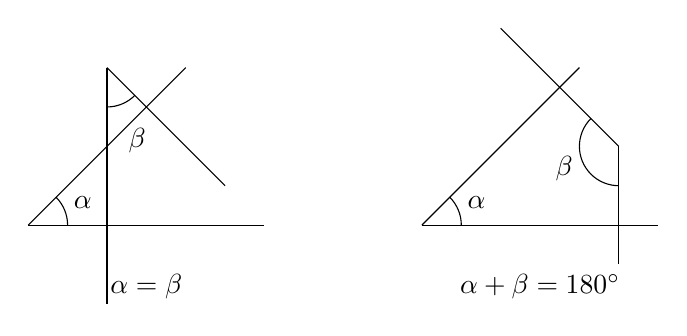
\begin{tikzpicture}
    \coordinate (A) at (1,0);
    \coordinate (B) at (4,0);
    \coordinate (C) at (3,2);

    \draw (A) -- (B);
    \draw (A) -- (C);
    \pic [draw, -, "$\alpha$", angle eccentricity=1.5] {angle = B--A--C};

    \coordinate (D) at (2,-1);
    \coordinate (E) at (2,2);
    \coordinate (F) at (3.5,0.5);

    \draw (D) -- (E);
    \draw (F) -- (E);

    \pic [draw, -, "$\beta$", angle eccentricity=2] {angle = D--E--F};

    \path (2.5,-0.5) node[below] {$\alpha = \beta$};

    \coordinate (A) at (5+1,0);
    \coordinate (B) at (5+4,0);
    \coordinate (C) at (5+3,2);

    \draw (A) -- (B);
    \draw (A) -- (C);
    \pic [draw, -, "$\alpha$", angle eccentricity=1.5] {angle = B--A--C};

    \coordinate (D) at (5+3.5,-1+0.5);
    \coordinate (E) at (5+2,2+0.5);
    \coordinate (F) at (5+3.5,0.5+0.5);

    \draw (F) -- (E);
    \draw (F) -- (D);

    \pic [draw, -, "$\beta$", angle eccentricity=1.5] {angle = E--F--D};
    \path (5+2.5,-0.5) node[below] {$\alpha + \beta = 180^{\circ}$};
\end{tikzpicture}


\subsubsection*{Notranji kot $\angle B A D$ trapeza $A B C D$, ki mu lahko očrtamo krožnico, meri $\alpha$. Koliko merijo ostali notranji koti tega trapeza?}

Trapezu ABCD smo očrtali krožnico, kar pomeni, da je trapez enakokrak. Iz česar sledi, da ima po dva para skladnih kotov: $\alpha=\beta$ in $\gamma=\delta$.

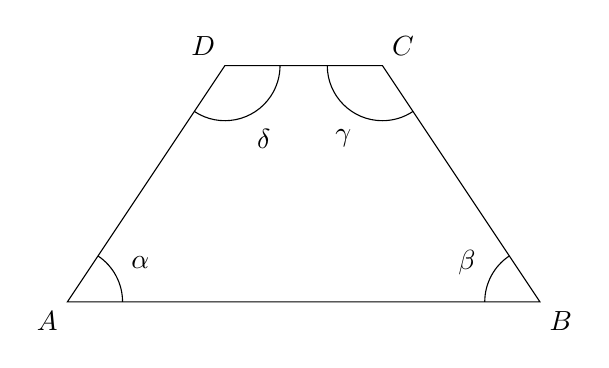
\begin{tikzpicture}
  % Define the coordinates of the trapezoid
  \coordinate (A) at (0,0);
  \coordinate (B) at (2*3,0);
  \coordinate (C) at (2*2,2*1.5);
  \coordinate (D) at (2*1,2*1.5);

  % Draw the trapezoid
  \draw (A) -- (B) -- (C) -- (D) -- cycle;

  % Label the vertices
  \node[below left] at (A) {$A$};
  \node[below right] at (B) {$B$};
  \node[above right] at (C) {$C$};
  \node[above left] at (D) {$D$};

  % Label the angles
  \draw pic["$\alpha$", draw=black, angle radius=7mm, angle eccentricity=1.5] {angle=B--A--D};
  \draw pic["$\beta$", draw=black, angle radius=7mm, angle eccentricity=1.5] {angle=C--B--A};
  \draw pic["$\gamma$", draw=black, angle radius=7mm, angle eccentricity=1.5] {angle=D--C--B};
  \draw pic["$\delta$", draw=black, angle radius=7mm, angle eccentricity=1.5] {angle=A--D--C};
\end{tikzpicture}

\section{Trikotnik}
\subsubsection*{Definirajte trikotnik.}

TRIKOTNIK, ki ga določajo poljubne tri nekolinearne točke $A$, $B$ in $C$, je konveksna množica točk v ravnini, omejena z daljicami $AB$, $AC$ in $BC$. Točke $A$, $B$ in $C$ imenujemo oglišča trikotnika, daljice $AB$, $AC$ in $BC$ pa stranice trikotnika. Če sta dve stranici trikotnika skladni, je trikotnik enakokrak, če so vse stranice trikotnika skladne, je enakostraničen.

\subsubsection*{Definirajte notranji in zunanji kot trikotnika.}

NOTRANJI kot trikotnika ima vrh v oglišču, kraka sta določena z drugima ogliščema in ves trikotnik leži v tem notranjem kotu. ZUNANJI kot trikotnika je sokot notranjega kota. Enak je vsoti njemu nepriležnih notranjih kotov $\left(\beta^{\prime}=\alpha+\gamma\right)$.

\subsubsection*{Kolikšna je vsota notranjih kotov trikotnika?}

Vsota notranjih kotov trikotnika je enaka $180^{\circ}$.

\subsubsection*{Kolikšna je vsota zunanjih kotov trikotnika? Trditev dokažite.}

Vsota zunanjih kotov trikotnikaje enaka $360^{\circ}$

\begin{proof}
    $\underline{\alpha}^{\prime}+\beta^{\prime}+\gamma^{\prime}=360^{\circ}$

    $$
\begin{aligned}
\alpha+\alpha^{\prime} = 180^{\circ} \\
\beta+\beta^{\prime} = 180^{\circ} \\
\gamma+\gamma^{\prime} = 180^{\circ} \\
\end{aligned}
$$

    $$
\begin{aligned}
& \left(\alpha+\alpha^{\prime}\right)+\left(\beta+\beta^{\prime}\right)+\left(\gamma+\gamma^{\prime}\right)=540^{\circ} \\
& (\alpha+\beta+\gamma)+\left(\alpha^{\prime}+\beta^{\prime}+\gamma^{\prime}\right)=540^{\circ} \\
& \left(\alpha^{\prime}+\beta^{\prime}+\gamma^{\prime}\right)=540^{\circ}-(\alpha+\beta+\gamma) \\
& \left(\alpha^{\prime}+\beta^{\prime}+\gamma^{\prime}\right)=540^{\circ}-180^{\circ} \\
& \left(\alpha^{\prime}+\beta^{\prime}+\gamma^{\prime}\right)=360^{\circ}
\end{aligned}
$$
\end{proof}

\section{Znamenite točke trikotnika}

\subsubsection*{Opišite konstrukcije simetrale daljice, simetrale kota in višine na stranico trikotnika.}

\textbf{Konstrukcija simetrale daljice:}

V šestilo vzamemo razdaljo večjo od polovice dolžine daljice in narišemo krožna loka s središčema v krajiščih $A$ in $B$. Skozi presečišči lokov narišemo pravokotno premico na daljico - simetralo daljiice.

\textbf{Konstrukcija simetrale kota:}

Narišemo krožni lok s središčem v vrhu kota in označimo njegovi presečǐšči s krakoma. Dobimo točki $A$ in $B$. Narišemo krožni lok s središčem v presečišču $A$. Narišemo krožni lok z enakim polmerom (kot iz točke A) s središčem v presečǐču B. Presečišče krožnih lokov označimo s C. Skozi točki V in C narišemo premico simetralo kota sa.

\textbf{Konstrukcija višine:}

Narišemo nosilko daljice $A B$ in jo označimo $p$. Narišemo pravokotnico na premico $p$ tako, da s šestilom, zapičenim v točko C, zarišemo tak krožni lok, ki dvakrat seka premico p. Presečišči poimenujemo $T_{1}$ in $T_{2}$. $V$ šestilo vzamemo dolžino, nekoliko večjo od polovične dolžine daljice $T_{1} T_{2}$. Šestilo zapičimo $v T_{1}$. S šestilom zarišemo krožni lok tako, da seka daljico $T_{1} T_{2}$. Ponovimo tako, da šestilo zapičimo v točko $T_{2}$. Ponovnooo zarišemo krožni lok, ki seka daljico $\mathrm{T}_{1} \mathrm{~T}_{2} \mathrm{n}$ obenem seka predhodnoo narisan lok. Točki, v katerih se sekata krožna loka, označimo s $P$ in $R$. $\mathrm{Z}$ ravnilom narišemo premico skozi točki $P$ in $R$ in jo označimo s q.mPresečišče premic $p$ in $q$ označimo s točko D. Daljica CD predstavlja višino trikotnika na stranico c.

\subsubsection*{Kako poiščemo središče trikotniku očrtanega kroga, središče trikotniku včrtanega kroga in višinsko točko trikotnika?}
\begin{itemize}
  \item Središče trikotniku očrtanega kroga je presečišče simetral stranic trikotnika.

  \item Središče trikotniku včrtanega kroga je presečǐče simetral notranjih kotov trikotnika.

  \item VIŠINSKA TOČKA trikotnika je presečišče (vsaj dveh) višin trikotnika oziroma nosilk višin, če je trikotnik topokoten.

\end{itemize}

\section{Skladnost likov}

\subsubsection*{Definirajte skladnost likov.}

Lika sta SKLADNA, če obstaja togi premik (vzporedni premik za nek vektor, vrtenje okrog neke točke, zrcaljenje čez točko ali čez premico), ki en lik preslika v drugega. Če sta lika skladna, imata paroma skladne stranice in paroma skladne kote.

\subsubsection*{Povejte štiri izreke o skladnosti trikotnikov.}

Trikotnika sta skladna, če:

\begin{enumerate}
  \item se ujemata v dveh stranicah in kotu med njima

  \item se ujemata v eni stranici in obeh kotih ob njej

  \item imata paroma skladne stranice

  \item se ujemata v dveh stranicah in kotu, ki leži nasproti daljši od teh stranic

\end{enumerate}

\subsubsection*{V paralelogramu narišemo eno diagonalo. Dokažite, da sta tako dobljena trikotnika skladna.}

\begin{proof}
    Dobljena trikotnika v paralelogramu, kjer smo narisali eno diagonalo, sta skladna.

    Paralelogram je štirikotnik, ki ima dva para vzporednih stranic.

    \begin{enumerate}
      \item stranca $A C$ je skupna $\triangle \mathrm{ABC}$ in $\triangle \mathrm{CDA}$
    
      \item $\overline{\mathrm{AD}}=\overline{\mathrm{BC}}$ (ker je $\mathrm{ABCD}$ paralelogram)
    
      \item $\overline{\mathrm{AB}}=\overline{\mathrm{CD}}$ (ker je $\mathrm{ABCD}$ paralelogram)
    
      \item $\triangle \mathrm{ABC}$ in $\triangle \mathrm{CDA}$ imata paroma skladne vse tri stranice, torej sta skladna.

\end{enumerate}

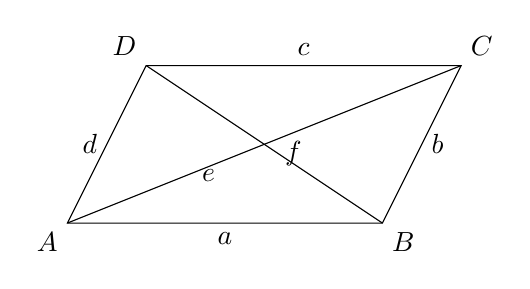
\begin{tikzpicture}
  % Define the coordinates of the parallelogram
  \coordinate (A) at (0,0);
  \coordinate (B) at (4,0);
  \coordinate (C) at (5,2);
  \coordinate (D) at (1,2);

  % Draw the parallelogram
  \draw (A) -- (B) -- (C) -- (D) -- cycle;

  % Label the points
  \node[below left] at (A) {$A$};
  \node[below right] at (B) {$B$};
  \node[above right] at (C) {$C$};
  \node[above left] at (D) {$D$};

  % Label the edges
  \node[below] at ($(A)!0.5!(B)$) {$a$};
  \node[right] at ($(B)!0.5!(C)$) {$b$};
  \node[above] at ($(C)!0.5!(D)$) {$c$};
  \node[left] at ($(D)!0.5!(A)$) {$d$};

  % Draw the diagonals
  \draw (A) -- (C);
  \draw (B) -- (D);

  % Label the diagonals
  \node[below left] at ($(A)!0.4!(C)$) {$e$};
  \node[above left] at ($(B)!0.3!(D)$) {$f$};
\end{tikzpicture}
\end{proof}


\section{\texorpdfstring{\cancel{Podobnost likov}}{Podobnost likov}}
\subsubsection*{Definirajte podobnost likov.}

Lika sta si podobna, če se da en lik na drugega preslikati s podobnostno preslikavo, tako da se popolnoma prekrijeta.
V podobnostne preslikave spadatajo
\begin{itemize}
    \item poljuben togi premik (ohranja razdalje med točkami)
    \item poljubno središčno preslikavo (ohranja kote, razdalje pa spreminja za faktor $k$)
    \item kompozitum togega premika in središčne preslikave
\end{itemize}

\subsubsection*{Povejte tri izreke o podobnosti trikotnikov.}

Dva trikotnika sta si podobna, če se ujemata:
\begin{enumerate}
    \item v dveh notranjih kotih
    \item v razmerjih po dveh enakoležnih stranic: $a : a_1 = b : b_1 = c : C_1 = k$
    \item v razmerju dveh stranic in kotu med njima 
\end{enumerate}

\subsubsection*{V pravokotnem trikotniku narišemo višino na hipotenuzo. Koliko podobnih trikotnikov nastane? Dokažite Evklidov ali višinski izrek.}

Višina v pravokotnem trikotniku razdeli trikotnika na dva manjša trikotnika, ki imata enake kote kot začetni trikotnik in so zato vsi trije med seboj podobni.

\textbf{Evklidov izrek}: Kvadrat katete je enak produktu hipotenuze in pravokotne projekcije te katete na hipotenuzo. 

\begin{proof}

\begin{figure}[H]
    \centering
    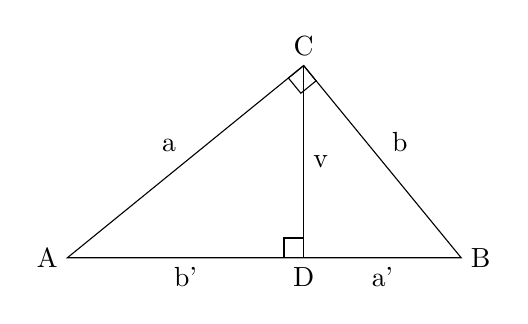
\begin{tikzpicture}
\coordinate (A) at (0, 0);
\coordinate (B) at (5, 0);
\coordinate (C) at (3, 2.44);
\coordinate (D) at (3, 0);

\draw (A) -- (B) -- (C) -- cycle;

\draw (C) -- (D);

\tkzMarkRightAngle(A,C,B);
\tkzMarkRightAngle(A,D,C);

\node[left] at (A) {A};
\node[right] at (B) {B};
\node[above] at (C) {C};
\node[below] at (D) {D};

\node[below] at ($(A)!0.5!(D)$) {b'};
\node[below] at ($(D)!0.5!(B)$) {a'};
\node[above left] at ($(A)!0.5!(C)$) {a};
\node[above right] at ($(B)!0.5!(C)$) {b};
\node[right] at ($(D)!0.5!(C)$) {v};
\end{tikzpicture}


\end{figure}

    \begin{gather*}
        \triangle ABC \approx \triangle ACD \\
        b : b' = c : b \\
        b^2 = b' \cdot c
    \end{gather*}

    \begin{gather*}
        \triangle ABC \approx \triangle CBD \\
        a : a' = c : a \\
        a^2 = a'\cdot c
    \end{gather*}
    
\end{proof}


\section{Paralelogram}
\subsubsection*{Definirajte paralelogram.}

PARALELOGRAM je štirikotnik, ki ima dva para vzporednih stranic.

\subsubsection*{Navedite lastnosti kotov in stranic paralelograma.}

Lastnosti stranic in kotov paralelograma:

\begin{enumerate}
    \item nasprotni stranici sta skladni in vzporedni
    \item po dva nasprotna kota sta skladna
    \item po dva sosednja kotaa sta suplementarna (skupaj merita $180^{\circ}$ )
\end{enumerate}

\subsubsection*{Navedite posebne vrste paralelogramov in opišite njihove lastnosti.}

Posebne vrste paralelogramov:
\begin{itemize}
    \item KVADRAT: paralelogram, ki je hkrati pravokotnik in romb, vsi notranji koti so pravi, vse stranice enako dolge, diagonali se sekata pravokotno in razpolavljata kota ob ogliščih, ki ju povezujeta
    \item PRAVOKOTNIK: paralelogram, ki ima štiri prave kote in enako dolgi diagonali
    \item ROMB: paralelogram, ki ima vse stranice enako dolge, diagonali se sekata pravokotno in razpolavljata kota ob ogliščih, ki ju povezujeta
\end{itemize}

\subsubsection*{Dokažite, da se diagonali v rombu sekata pod pravim kotom.}

\begin{proof}
     Diagonali v rombu se sekata pod pravim kotom.

     A, B, C, D so oglišča romba, S je središče (presečišče diagonal)

     Trikotnika ABS in CBS sta skladna, ker se ujemata v istoležnih stranicah $(A B \cong$ $\mathrm{BC}, \mathrm{AS} \cong \mathrm{SC}, \mathrm{BS} \cong \mathrm{BS})$, zato je $\angle \mathrm{ASB} \cong \angle \mathrm{CSB}$. Ker sta $\angle \mathrm{ASB}$ in $\angle \mathrm{CSB}$ sokota, merita vsak po $90^{\circ}$. Diagonali se sekata pravokotno.
\end{proof}
 

\section{Trapez}
\subsubsection*{Definirajte trapez.}

TRAPEZ je štirikotnik, ki ima par vzporednih stranic. Vzporedni stranici sta osnovnici, preostali dve sta kraka.

\subsubsection*{Navedite lastnosti kotov trapeza.}

Notranja kota ob istem kraku sta suplementarna $\left(\alpha+\delta=180^{\circ}, \beta+\gamma=180^{\circ}\right)$. Vsota notranjih kotov je enaka $360^{\circ}$.

\subsubsection*{Kaj je srednjica trapeza in katere lastnosti ima?}

 Srednjica trapeza je zveznica razpolovišč krakov in je vzporedna z osnovnicama, njena dolžina je enaka aritmetični sredini dolžin obeh osnovnic: $s=\frac{a+c}{2}$

\subsubsection*{Pri katerih trapezih sta diagonali enako dolgi? Naj bo $S$ presečišče diagonal takšnega trapeza. Izrazite razmerje dolžin $|A S|:|S C|$ z dolžinama osnovnic trapeza, kjer je $A C$ ena izmed diagonal trapeza.}

Diagonali sta enako dolgi v enakokrakem trapezu. 

S je presečišče diagonal. Diagonali sta $|A C|=e,|B D|=f$ in $e=f$.

$$
\begin{aligned}
& |A S|:|S C|=? \\
& |A S|=|D S|=e_{1} \\
& |S C|=|S B|=\mathrm{e}_{2} \\
& \mathrm{e}_{1}+\mathrm{e}_{2}=\mathrm{e} \\
& \Delta \mathrm{ADS} \sim \Delta \mathrm{CBS} \\
& \frac{a}{c}=\frac{e_{\mathbf{1}}}{e_{\mathbf{2}}}
\end{aligned}
$$

\section{Premice in krožnice}
\subsubsection*{V kakšni medsebojni legi sta lahko premica in krožnica, ki ležita v isti ravnini?}
Premica in krožnica, ki ležita na isti ravnini:
\begin{itemize}
  \item nimata nobene skupne točka (MIMOBEŽNICA)

  \item imata eno skupno točko (TANGENTA)

  \item imata dve različni skupni točki (SEKANTA)

\end{itemize}

\subsubsection*{Podrobno opišite konstrukcijo tangente na krožnico skozi dano točko zunaj krožnice.}

Dana je krožnica s središčem S in točka T zunaj krožnice.

Ker je tangenta pravokotna na polmer krožnice, ki povezuje dotikališče s središčem krožnice, načrtamo pravokoten trikotnik s hipotenuzo ST. Upoštevamo, da je vsak obodni kot nad premerom pravi, zato poiščemo razpolovišče $P$ daljice $S T$ in narišemo krožnico s središčem v točki $P$ in polmerom $|P T|$. Ta krožnica seka dano krožnico v točkah $D_{1}$ in $D_{2}$, ki sta dotikališči tangent. Skozi točko T torej lahko načrtamo dve tangenti na dano krožnico. Ker sta tangenti na krožnico pravkotoni, sta pravokotna tudi trikotnika $\Delta \mathrm{SD}_{1} \mathrm{~T}$ in $\Delta \mathrm{SD}_{2} \mathrm{~T}$.

\section{Središčni in obodni kot}
\subsubsection*{Definirajte središčni in obodni kot v krogu.}

SREDIŠČNI KOT $(\alpha)$ nad lokom je kot, katerega vrh je središče krožnice, kraka pa gresta skozi točki, ki določata lok.

OBODNI KOT $(\varphi)$ nad lokom je kot, ki ima vrh na krožnici, kraka pa gresta skozi točki, ki določata lok.

\subsubsection*{V kakšni zvezi sta, če ležita nad istim lokom v krogu?}

$\alpha=2 \varphi$ Središčni kot je dvakrat toliko velik kot obodni kot nad istim lokom. Vsi obodni koti nad istim lokom so enako veliki.

\subsubsection*{Povejte in dokažite Talesov izrek o kotu v polkrogu.}

\textbf{Talesov izrek o kotu v polkrogu:} \textit{Kot, ki ima vrh na krožnici, kraka pa potekata skozi krajišči premera te krožnice, je pravi kot.}

\begin{proof}
    Talesov izrek o kotu v polkrogu

    Trikotnika $\triangle AST$ in $\triangle SBT$ sta enakokraka, kjer so stranice $|AS|$, $|SB|$, $|ST|$ enake $r$. Koti $\angle SBT = \angle BTS$ in $\angle TAS = \angle STA$. Kota $\angle AST$ in $\angle BST$ sta komplementarna. 
    \begin{align*}
        \angle AST &= 180^\circ - 2\alpha \\
        \angle BST &= 180^\circ - \angle AST = 180^\circ - (180^\circ - 2\alpha) = 2\alpha
    \end{align*}

    % TODO: A je to dovolj dober dokaz al bi blo treba dokazat tut to da je alfa = 2fi? Recimo tist drug PDF ima en dokaz z enakokrakimi trikotniki pa to ... - nov dokaz iz wikipedia.com
    \begin{center}
    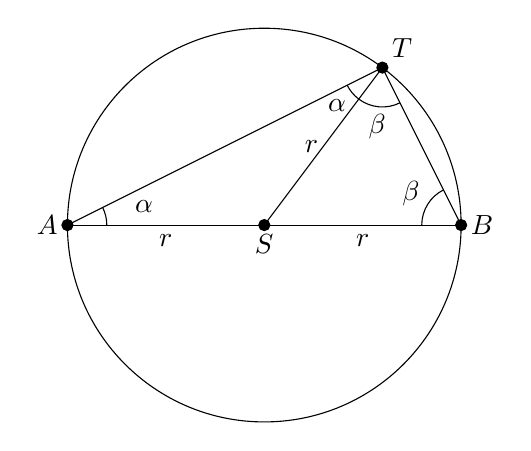
\begin{tikzpicture}
        \coordinate (O) at (0, 0);
        \coordinate (T) at (3/2, 4/2);
        \coordinate (A) at (-5/2, 0);
        \coordinate (B) at (5/2, 0);
        \draw (O) circle (5/2);
        \draw (A) -- (B);
        \filldraw (T) circle[radius=2pt] node[above right]{$T$};
        \filldraw (O) circle[radius=2pt] node[below]{$S$};
        \filldraw (A) circle[radius=2pt] node[left]{$A$};
        \filldraw (B) circle[radius=2pt] node[right]{$B$};
        \draw (O) -- (T);
        \node[above] at ($(O)!0.4!(T)$) {$r$};
        \node[below] at ($(O)!0.5!(B)$) {$r$};
        \node[below] at ($(A)!0.5!(O)$) {$r$};
        \draw (T) -- (B);
        \draw (A) -- (T);
        \pic [draw, -, "$\alpha$", angle eccentricity=2] { angle = B--A--T };
        \pic [draw, -, "$\alpha$", angle eccentricity=1.5] { angle = A--T--O };

        \pic [draw, -, "$\beta$", angle eccentricity=1.5] { angle = O--T--B };
        \pic [draw, -, "$\beta$", angle eccentricity=1.5] { angle = T--B--O };
    \end{tikzpicture}
    \end{center}
\end{proof}
\subsubsection*{Kako uporabimo Talesov izrek pri konstrukciji pravokotnega trikotnika s podano hipotenuzo in višino na hipotenuzo?}

Talesov izrek pri konstrukciji pravokotnega trikotnika s podano hipotenuzo in višino na hipotenuzo uporabimo tako, da najprej narišmo hipotenuzo, katere dolžina nam je podana. Nato skonstruiramo njeno središče s pomočjo simetrale. Razdalja $|A S|=$ $|S B|$ je enaka polmeru krožnice, ki jo zrišemo. Ker imamo podano višino, lahko narišemo vzporednico hipotenuzi, ki je od nje oddaljena za dolžino višine. Kjer sta presečišči krožnice $z$ vporednico, tam sta $C_{1}$ in $C_{2}$, torej dve možni oglišči trikotnika. Narišemo trikotnika $\triangle \mathrm{ABC}_{1}$ in $\triangle \mathrm{ABC}_{2}$.

\section{Sinusni in kosinusni izrek}
\subsubsection*{Povejte kosinusni izrek. Na primeru opišite njegovo uporabo.}

Kvadrat stranice trikotnika je enak vsoti kvadratov drugih dveh stranic, zmanjšani za dvakratni produkt teh dveh stranic in kosinusa kota med njima. V poljubnem trikotniku s stranicami $a, b, c$ in nasproti ležečimi koti $\alpha, \beta, \gamma$ torej velja:

$$
\begin{aligned}
& a^{2}=b^{2}+c^{2}-2 b c \cdot \cos \alpha \\
& b^{2}=a^{2}+c^{2}-2 a c \cdot \cos \beta \\
& c^{2}=a^{2}+b^{2}-2 a b \cdot \cos \gamma
\end{aligned}
$$

\paragraph{Primer:}

\begin{multicols}{2}
\begin{align*}
    a &= 4 cm \\
    b &= 5 cm \\
    \gamma &= 60^\circ
\end{align*} \columnbreak
\begin{align*}
    \\
    c^2 &= a^2 + b^2 - 2ab\cos \gamma = 13 \\
    c &= \sqrt{13} cm
\end{align*}
\end{multicols}

Uporaba:

\begin{itemize}
  \item če sta znani dve stranici in kot med njima (izračunamo tretjo stranico)
  \item če so znane vse tri stranice trikotnika (izračunamo vse kote trikotnika)
\end{itemize}

% TODO: Primer is left as an exercise to the reader? - primer je dodan

\subsubsection*{Povejte sinusni izrek. Na primeru opišite njegovo uporabo.}

Razmerje med dolžino stranice in sinusom njej nasprotnega kota je enako za vse tri stranice v trikotniku. To razmerje je enako dvakratniku polmera trikotniku očrtanega kroga. V poljubnem trikotniku s stranicami $a, b, c$ in nasproti ležečimi koti $\alpha, \beta, \gamma$ torej velja:

$$
\begin{aligned}
\frac{a}{\sin\alpha} = \frac{b}{\sin\beta} = \frac{c}{\sin\gamma} = 2R
\end{aligned}
$$

\paragraph{Primer:}

\begin{center}

\begin{tabular}{ p{5
cm} l }
     $R = 5 cm$ &  $a = 2R \cdot \sin{\alpha} = 10 \cdot 0.5 = 5 cm$\\
     $\alpha = 30^\circ$ & $b = 2R \cdot \sin{\beta} = 10 \cdot \frac{\sqrt{3}}{2} = 5\sqrt{3} cm$ \\
     $\beta = 60^\circ$ & $c = 2R \cdot \sin{\gamma} = 10 \cdot 1 = 10 cm$     
\end{tabular}
    
\end{center}
Uporaba:

\begin{itemize}
  \item če je znana stranica in dva notranja kota (ena rešitev)
  \item če sta znani dve stranici in kot nasproti večje stranice (ena rešitev)
  \item če sta znani dve stranici in kot nasproti manjše stranice (dve, ena ali nič rešitev)
  \item če je znan polmer očrtanega kroga in dve stranici
  \item če je znan polmer očrtanega kroga in dva notranja kota
\end{itemize}

% TODO: Primer is left as an exercise to the reader? - dodan

\subsubsection*{Dokažite enega izmed zgornjih izrekov.}

\begin{proof}
    $V$ trikotniku $A B C$ je kot $\angle A C B$ obodni kot nad lokom $A B$, kot $\angle A S B$ pa pripadajoči središčni kot nad istim lokom. Trikotnik ABS je enakokrak, zato višina na osnovnico razpolavlja kot ob vrhu - vsak od obeh delov ima zato velikost $\gamma$. Tedaj je:

$\sin \gamma=\frac{\frac{c}{2}}{R} \Rightarrow c=2 R \cdot \sin \gamma \Rightarrow \frac{c}{\sin \gamma}=2 R$

$\sin \alpha=\frac{\frac{a}{2}}{R} \Rightarrow a=2 R \cdot \sin \alpha \Rightarrow \frac{a}{\sin \alpha}=2 R$

$\sin \beta=\frac{\frac{b}{2}}{R} \Rightarrow b=2 R \cdot \sin \beta \Rightarrow \frac{b}{\sin \beta}=2 R$

Dokazali smotrditev $\frac{a}{\sin \alpha}=\frac{b}{\sin \beta}=\frac{c}{\sin \gamma}=2 R$.
\end{proof}

\section{Ploščine likov}
\subsubsection*{Navedite formulo za izračun ploščine trikotnika.}

$$
S=\frac{a \cdot v_{a}}{2}=\frac{a \cdot b \cdot \sin \gamma}{2}=\sqrt{s(s-a)(s-b)(s-c)}=2 R^{2} \cdot \sin \alpha \cdot \sin \beta \cdot \sin \gamma
$$

$$
s = \frac{a + b+ c}{2}
$$

\subsubsection*{Navedite formulo za izračun ploščine paralelograma.}

$$
S=a \cdot v_{a}=b \cdot v_{b}=a \cdot b \cdot \sin \alpha=a \cdot b \cdot \sin \beta
$$


\subsubsection*{Navedite formulo za izračun ploščine deltoida in jo dokažite.}

$$
S=\frac{e \cdot f}{2}
$$

\begin{proof}
    Imamo deltoid $A B C D \mathrm{z}$ diagonalama e in $\mathrm{f}$.

Ker se diagonali deltoida sekata pravokotno, pri čemer ena diagonala razpolavlja drugo, lahko polovico deltoida razrežemo v dva trikotnika in oblikujemo pravokotnik, ki ima enako ploščino kot deltoid. Ploščina deltoida je torej enaka $S=\frac{\text { e.f }}{2}$.
\end{proof}

\subsubsection*{Navedite formulo za izračun ploščine trapeza in jo dokažite.}

$$
\begin{aligned}
& S=\frac{(a+c) \cdot v}{2}=s \cdot v \\
& s=\frac{a+c}{2}
\end{aligned}
$$

\begin{proof}
    Imamo trapez ABCD z osnovnicama a in c ter višino v.

Če skladna trapeza zlepimo vzdolž enako dolgih krakov, dobimo paralelogram z enako višino v kot trapez, dolžina stranice paralelograma pa je enaka vsoti dolžin osnovnic trapeza. Ploščina paralelograma je enaka $(a+c) \cdot v$. Ploščina trapeza je enaka polovici ploščine paralelograma, in sicer $S=\frac{(a+c) \cdot v}{2}$.

Dolžina zveznice razpolovišč/srednjice je enaka aritmetični sredini dolžin osnovnic.
\end{proof}
\section{Ploščine likov}
\subsubsection*{Navedite formuli za izračun ploščine kvadrata in ploščine pravokotnika.}

Formuli za izračun ploščine KVADRATA:

$$
S=a^{2}=\frac{d^{2}}{2}
$$

Formula za izračun ploščine PRAVOKOTNIKA:

$$
S=a \cdot b
$$

\subsubsection*{Navedite formulo za izračun ploščine romba in jo dokažite.}

$$
S=a \cdot v_{a}=a^{2} \cdot \sin \alpha=\frac{e \cdot f}{2}
$$

\begin{proof}
    Imamo romb $A B C D$ s stranico a in višino $v_{a}$.

    Če v romb narišemo njegovo višino $v_{a}$, ga razdelimo na pravkotni trikotnik in pravokotni trapez. Izrezan trikotnik primaknemo $\mathrm{k}$ trapezu tako, da postavimo hipotenuzo na k njej vzporednemu kraku trapeza, ki ima prav tako dolžino a. Dobimo pravokotnik s stranicama a in $v_{a}$. Zato ploščino izračunamo $\operatorname{kar} S=a \cdot v_{a}$.
\end{proof}

\subsubsection*{Izpeljite formulo za izračun višine enakostraničnega trikotnika.}

Imamo enakostraničen trikotnik s stranico a in višino v. Formula za izračun ploščine trikotnika je $S=\frac{a \cdot v_{a}}{2}$. Z višino trikontik razdelimo na dva skladna pravokoktna trikotnika, katerih hipotenuza je enaka stranici a, ena izmed katet je enaka polovici stranice a, druga kateta pa je enaka višini.

$$
\begin{aligned}
& a^{2}=v_{a}^{2}+\left(\frac{a}{2}\right)^{2} \\
& v_{a}=\sqrt{a^{2}-\left(\frac{a}{2}\right)^{2}}=\frac{2 \mathrm{~s}}{a}=\frac{a \sqrt{3}}{2}
\end{aligned}
$$

\subsubsection*{Navedite formuli za izračun ploščine enakostraničnega in ploščine pravokotnega trikotnika.}

$$
S=\frac{a^{2} \sqrt{3}}{4}
$$

Formuli za izračun ploščine PRAVOKOTNEGA TRIKOTNIKA:

$$
S=\frac{a \cdot b}{2}=\frac{c \cdot v_{c}}{2}
$$

\section{Krog}

\subsubsection*{Navedite formuli za izračun ploščine in obsega kroga.}

$$
\begin{aligned}
& S=\pi \cdot r^{2} \\
& o=2 \cdot \pi \cdot r
\end{aligned}
$$

\subsubsection*{Povejte in izpeljite formulo za izračun dolžine krožnega loka.}

V krogu z danim polmerom je dolžina krožnega loka premo sorazmerna velikosti središčnega kota. Zato lahko s križnim računim izpeljemo formulo:

$2 \pi r \ldots 360^{\circ}$

$1 \ldots \alpha$

$1 \cdot 360^{\circ}=2 \pi r \cdot \alpha$

$l=\frac{2 \pi r \alpha}{360^{\circ}}$

$1=\frac{\pi r \alpha}{180^{\circ}}$

\subsubsection*{Povejte in izpeljite formulo za izračun ploščine krožnega izseka.}

Krožni izsek je del kroga, ki ga omejujejo dva polmera in krožni lok. Njegova ploščina je premo sorazmerna z velikostjo središčnega kota. Če središcni kot meri $\alpha$ stopinj, potem je ploščina krožnega izseka enaka $\frac{\alpha}{360^{\circ}}$ ploščine celotmega kroga. Velja:

$S=\pi r^{2} \cdot \frac{\alpha}{360^{\circ}}=\frac{\pi r^{2} \alpha}{360^{\circ}}$

$S=\frac{r \cdot l}{2}$

\section{Prizma}
\subsubsection*{Definirajte prizmo.}

PRIZMA je oglato telo, katerega vzporedni mejni ploskvi sta skladna večkotnika. Vzporedni robovi povezujejo vsako oglišče enega večkotnika z ogliščem drugega. Vzporedni mejni ploskvi, ki sta skladna večkotnika, sta osnovni ploskvi prizme. Druge mejne ploskve so stranske ploskve. Vse stranske ploskve skupaj oblikujejo plašč prizme. Osnovni robovi so stranice osnovne ploskve prizme. Stranski robovi so vsi med seboj vzporedni robovi, ki povezujejo oglišča ene osnovne ploskve z oglišči druge osnovne ploskve. Prizmo poimenujejo po številu stranic osnovne ploslve. Višina prizme je razdalja med ravninama osnovnih ploskev. Diagonala prizme je zveznica dveh oglišč, ki ne ležita na iistii ploskvi (kocka, kvader).

\subsubsection*{Kdaj je prizma, enakoroba, $n$-strana, pravilna?}

\begin{itemize}

  \item Prizma je ENAKOROBA, če so vsi njeni robovi enako dolgi.

  \item Prizma je N-STRANA, če ima n osnovnih robov oz. je njena osnovna ploskev n-kotnik

  \item Prizma je PRAVILNA, če je pokončna in ima za osnovni ploskvi pravilna lika.
\end{itemize}



\subsubsection*{Navedite formuli za izračun prostornine in površine pokončne prizme.}

$V=S \cdot v$

$p=2 \cdot S+\mathbf{p l}$

$\mathbf{p l}=o \cdot v$

v - višina prizme, pl - ploščina plašča, o - obseg osnovne ploskve, S - ploščina osnovne ploske

\subsubsection*{Izpeljite formulo za izračun prostornine pravilne enakorobe šeststrane prizme z robom $a$}

Prostornino izračunamo po formuli $V=S \cdot v$. Osnovna ploskev je pravilni šestkotnik, njena ploščina je $S=\frac{6 \cdot a^{2} \sqrt{3}}{4}=\frac{a^{2} \cdot 3 \sqrt{3}}{2}$. Višina pa je enaka osnovnemu robu, torej meri a. Formula za prostornino je torej:

$\mathrm{V}=\mathrm{S} \cdot \mathrm{V}$

$\mathrm{V}=\frac{a^{2} \cdot 3 \sqrt{3}}{2} \cdot a$

$V=\frac{a^{3} 3 \sqrt{3}}{2}$ 

\section{Valj}

\subsubsection*{Definirajte pokončni valj.}

POKOČNI VALJ je rotacijsko telo, ki nastane tudi z vrtenjem pravokotnika okoli ene od stranic za $360^{\circ}$ ali ene od obeh simetrijskih osi za $180^{\circ}$. Omejujeta ga dva enaka vzporedna skladna kroga (osnovni ploskvi) in plašč v obliki sklenjene valjaste ploskve. Premica, ki gre skozi središči obeh osnovnh ploskev, je os valja. Razdalja, med obema osnovnima ploskvama, pa višina v valja.

\subsubsection*{Skicirajte mrežo valja.}

\begin{tikzpicture}
  \draw (2,0) circle [radius=1];
  \draw (0,1) rectangle (3.14*2,3);
  \draw (3.14*2,2) node[right] {v};
  \draw (4,3) node[above] {$2\pi r$};
  \draw (2,4) circle [radius=1];
  \draw (2,4) -- (3, 4);
  \node[above] at ($(2,4)!0.5!(3, 4)$) {$r$};
\end{tikzpicture}

\subsubsection*{Kaj je osni presek valja?}

Če valj presekamo z ravnino, ki gre skozi njegovo os, dobimo OSNI PRESEK valja.

\subsubsection*{Navedite formuli za izračun površine in prostornine pokončnega valja.}

$$
\begin{aligned}
& V=S \cdot V=\pi \cdot r^{2} \cdot v \\
& p=2 S+p l=2 \pi \cdot r^{2}+2 \pi \cdot r \cdot v=2 \pi \cdot r \cdot(r+v)
\end{aligned}
$$

\subsubsection*{Izpeljite formulo za izračun površine valja.}

$$
\begin{aligned}
& p=2 S+p l=2 \pi \cdot r^{2}+2 \pi \cdot r \cdot v=2 \pi \cdot r \cdot(r+v)
\end{aligned}
$$

\subsubsection*{Izrazite prostornino enakostraničnega valja s polmerom osnovne ploskve $r$.}

Polmer je $r$, višina valja je enaka ravno $2 r$. Formula je $V=S \cdot V=\pi \cdot r^{2} \cdot v$, torej v našem primeru $V=\pi \cdot r^{2} \cdot \mathbf{2 r}=2 \pi r^{3}$.

\section{Piramida}
\subsubsection*{Definirajte piramido.}

PIRAMIDA je oglato telo, kateregaosnovna ploskev je večkotnik, stranske ploskve pa so trikotniki,ki se stikajo v skupni točki, ki jo imenujemo vrh piramide. Vse stranske ploskve skupaj oblikujejo plašč piramide. Stranice osnovne ploskve so osnovni robovi. Rob, v katerem se stikata dve stranski ploskvi, je stranski rob. Višine piramide je razdalja vrha od osnovne ploskve. Stranska višina je višina stranske ploskve. Piramido poimenujemo po številu stranic osnovne ploskve.

\subsubsection*{Kdaj je piramida enakoroba, $n$-strana, pravilna?}

\begin{itemize}
  \item Piramda je ENAKOROBA, če so vsi injeni robovi enako dolgi.

  \item Piramida je N-STRANA, če ima je njena osnovna ploskev n-kotnik.

  \item Piramida je PRAVILNA, če je pokončna in ima za osnovno ploskev pravilni n-kotnik.

\end{itemize}

\subsubsection*{Navedite formuli za izračun površine in prostornine pravilne piramide.}

$V=\frac{s \cdot v}{3}=\frac{n}{6} \cdot R^{2} \cdot v \cdot \sin \frac{360^{\circ}}{n}$

$P=S+p l=S+\frac{n \cdot a \cdot v_{1}}{2}=\frac{n}{2} \cdot R^{2} \cdot \sin \frac{360^{\circ}}{n}+n \cdot R \cdot v_{1} \cdot \sin \frac{180^{\circ}}{n}$

$\mathrm{V}_{1}$ - višina stranske ploskve, $\mathrm{R}$ - polmer pravilnemu n-kotniku očrtanega kroga, $S$ - ploščina osnovne ploskve, v - višina ploskve


\subsubsection*{Izrazite prostornino pravilne enakorobe tristrane piramide z robom $a$.}

Osnovna ploskev je enakostranični trikotnik s stranico a. Stranski robovi so enake dolžine kot osnovni robovi oziroma stranica trikotnika (a). Formula za prostornino je $V=\frac{S \cdot v}{3}$, torej v našem primeru $V=\frac{\frac{a^{2} \sqrt{3}}{4} \cdot v}{3}=\frac{a^{2} \sqrt{3} \cdot v}{12}=\frac{a^{2} \sqrt{3} \cdot a \sqrt{6}}{12 \cdot 3}=\frac{a^{3} \cdot \sqrt{2}}{12}$. $\mathrm{v}_{a}=\frac{a \sqrt{3}}{2}, \mathrm{v}=\frac{a \sqrt{6}}{3}$

$v_{a}$ - višina stranske ploskve, v - višina piramide

\section{Stožec}
\subsubsection*{Definirajte pokončni stožec.}


POKONČNI STOŽEC je geometrijsko telo, omejeno s krogom in krivo ploskvijo.

Osnovna ploskev je krog, katerega polmer r imenujemo polmer stožca. Točka $V$ je vrh stožca, daljica, ki veže vrh stožca in točko na robu osnovne ploskve, je stranica stožca. Plašč stožca je krožni izsek, katerega lok je enak obsegu osnovne ploskve, polmer pa stranici stožca. Razdalja vrha stožca od osnovne ploskve je višina stožca. Stožec je pokončen, ko je os stožca (premica, ki gre skozi vrh in središče osnovne ploskve)pravokotna na ravnino osnovne ploskve, sicer je poševen.

\subsubsection*{Skicirajte mrežo stožca.}

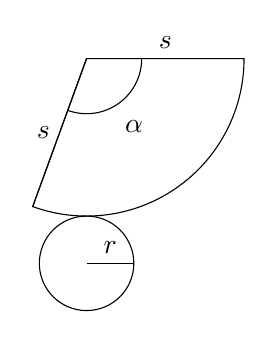
\begin{tikzpicture}
% Circle parameters
\def\centerX{0} % X-coordinate of the circle center
\def\centerY{0} % Y-coordinate of the circle center
\def\radius{2} % Circle radius

% Specify the angle range for the part of the circle (in degrees)
\def\startAngle{250}
\def\endAngle{360}

% Draw the part of the circle
\draw (\centerX, \centerY) -- (\startAngle:\radius) arc (\startAngle:\endAngle:\radius) -- cycle;

% Label the angles
\draw (\centerX, \centerY) -- (\startAngle:\radius);
\draw (\centerX, \centerY) -- (\endAngle:\radius);

\draw (0, -2.6) circle [radius=0.6];
\draw (0, -2.6) -- (0.6, -2.6);
\node[above] at ($(0, -2.6)!0.5!(0.6, -2.6)$) {$r$};

\node[left] at ($(\centerX, \centerY)!0.5!(\startAngle:\radius)$) {$s$};
\node[above] at ($(\centerX, \centerY)!0.5!(\endAngle:\radius)$) {$s$};

\coordinate (A) at (\startAngle:\radius);
\coordinate (B) at (\centerX, \centerY);
\coordinate (C) at (\endAngle:\radius);
    
\draw pic["$\alpha$", draw=black, angle radius=7mm, angle eccentricity=1.5] {angle=A--B--C};
\end{tikzpicture}

\subsubsection*{Opišite presek stožca z ravnino, vzporedno osnovni ploskvi.}

PRESEK stožca z ravnino, vzporedno osnvoni ploskvi, je krog, ki je podoben osnovni ploskvi.

\subsubsection*{Opišite presek stožca z ravnino, ki vsebuje os stožca.}

PRESEK stožca z ravnino, ki vsebuje os stožca, je enakokraki trikotnik z osnovnico $2 r$ in krakom s (stranica stožca) in ga imenujemo osni presek stožca.

\subsubsection*{Navedite formuli za površino in prostornino stožca.}

$$
\begin{aligned}
& V=\frac{s \cdot v}{3}=\frac{\pi r^{2} \cdot v}{3} \\
& p=S+\mathbf{p l}=\pi r^{2}+\pi \mathbf{r s}=\pi r(r+s)
\end{aligned}
$$

\subsubsection*{Izrazite površino enakostraničnega stožca s polmerom $r$.}

$$
P=S+p l=\pi r^{2}+\pi r s=\pi r^{2}+\pi r \cdot 2 r=3 \pi r^{2}
$$

\section{Vektorji}
\subsubsection*{Kaj je vektor?}

VEKTOR je matematična količina, ki jo ponazorimo z usmerjeno daljico. Ima velikost, smer in usmerjenost. Usmerjena daljica $\overrightarrow{\mathrm{AB}}$ je daljica, ki ima začetno točko $A$ in končno točko $B$.

\subsubsection*{Definirajte seštevanje vektorjev.}

Seštevanje vektorjev je operacija, ki paru vektorjev $(\vec{a}, \vec{b})$, priredi vsoto $\vec{a}+\vec{b}$. Za seštevanje vektorjev uporabljamo paralelogramsko ali trikotniško pravilo.

\subsubsection*{Definirajte ničelni vektor in nasprotni vektor danega vektorja.}

\begin{enumerate}
    \item NIČELNI VEKTOR je vektor, ki ima začetno točko enako končni. (primer: $\overrightarrow{A A}$ )

  \item NASPROTNI VEKTOR je vektor, ki ima glede na prvotni vektor enako dolžino in smer, vendar nasprotno usmerjenost. (primer: $\overrightarrow{A B}=-\overrightarrow{B A}$ )
\end{enumerate}

\subsubsection*{Povejte vsaj dve lastnosti seštevanja vektorjev in vsaj eno izmed njih dokažite.}

\begin{enumerate}
    \item ASOCIATIVNOST: $(\overrightarrow{a}+\overrightarrow{b})+\overrightarrow{c}=\overrightarrow{a}+(\overrightarrow{b}+\overrightarrow{c})$
    \item KOMUTATIVNOST: $\overrightarrow{a}+\overrightarrow{b}=\overrightarrow{b}+\overrightarrow{a}$
\end{enumerate}
\begin{proof}
    Seštevanje vektorjev je komutativno.

    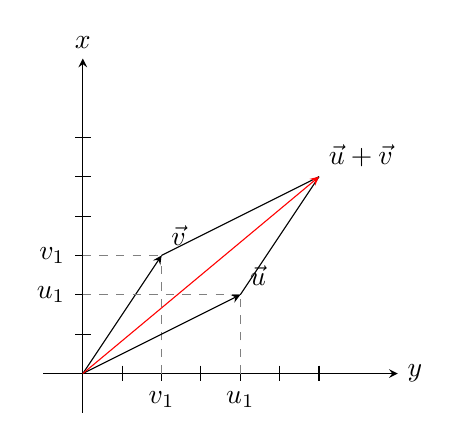
\begin{tikzpicture}
    % Draw axes
    \draw[->] (-0.5,0) -- (4,0) node[right] {$y$};
    \draw[->] (0,-0.5) -- (0,4) node[above] {$x$};

    % Label x-axis ticks
    \foreach \x in {0.5,1, 1.5, 2, 2.5, 3}
        \draw (\x,0.1) -- (\x,-0.1);

    % Label y-axis ticks
    \foreach \y in {0.5,1, 1.5, 2, 2.5, 3}
        \draw (0.1,\y) -- (-0.1,\y);

    \draw (1,0.1) -- (1,-0.1) node[below] {$v_1$};
    \draw (0.1,1.5) -- (-0.1,1.5) node[left] {$v_1$};
    \draw[gray, dashed] (1, 0) -- (1, 1.5);
    \draw[gray, dashed] (0, 1.5) -- (1, 1.5);
    \draw[->] (0,0) -- (1,1.5);

    \fill (1,1.5) node[above right] {$\vec{v}$};

    \draw (2,0.1) -- (2,-0.1) node[below] {$u_1$};
    \draw (0.1,1) -- (-0.1,1) node[left] {$u_1$};
    \draw[gray, dashed] (2, 0) -- (2,1);
    \draw[gray, dashed] (0, 1) -- (2,1);
    \draw[->] (0,0) -- (2,1);

    \fill (2,1) node[above right] {$\vec{u}$};
    \draw[-] (2,1) -- (3, 2.5);
    \draw[-] (1, 1.5) -- (3, 2.5);

    \fill (3,2.5) node[above right] {$\vec{u} + \vec{v}$};
    \draw[->, red] (0, 0) -- (3, 2.5);
\end{tikzpicture}

Dokažemo grafično (z enim izmed pravil), saj vsota pride isti vektor, ne glede na vrstni red risanja vektorjev (kot prikazuje zgornja skica).
\end{proof}


\section{Vektorji}
\subsubsection*{Definirajte množenje vektorjev s skalarji.}

Množenje vektorjev s številom (skalarjem) je dvočlena operacija; produkt vektorja $\vec{a} z$ realnim številom $\mathrm{k}$ je vektor $\mathrm{k} \cdot \overrightarrow{a}$. Vektorja $\overrightarrow{a}$ in $\mathrm{k} \cdot \overrightarrow{a}$ sta vzporedna. Vektor $\mathrm{k} \cdot \overrightarrow{a}$ kaže v isto smer kot $\vec{a}$, če je $k>0$, in kaže v nasprotno smer, če je $k<0$.

\subsubsection*{Povejte vsaj dve lastnosti množenja vektorjev s skalarji in vsaj eno izmed njih dokažite.}

\begin{enumerate}
    \item ASOCIATIVNOST V SKALARNEM FAKTORJU: $k(l \cdot \overrightarrow{a})=(k \cdot l) \cdot \overrightarrow{a}$
    \item DISTRIBUTIVNOST V SKALARNEM FAKTORJU: $(k+l) \cdot \overrightarrow{a}=k \cdot \overrightarrow{a}+l \cdot \overrightarrow{a}$
    \item DISTRIBUTIVNOST V VEKTORSKEM FAKTORJU: $(\overrightarrow{a}+\overrightarrow{b}) \cdot k=k \cdot \overrightarrow{a}+k \cdot \overrightarrow{b}$
\end{enumerate}

\begin{proof}
    Množenje vektorjev je asociativno v skalarnem faktorju.

    Vseeno je, ali vektor najprej pomnožimo s skalarjem $k$, nato pa še dobljeni vektor s skalarjem I, ali pa če vektor že na začetku pomnožimo s produktom skalarjev $k$ in $I$.
\end{proof}

\subsubsection*{Kdaj sta vektorja kolinearna?}

Vektorja sta KOLIENARNA, če imata isto smer (to je vektorja $\vec{a}$ in $\vec{b}$ sta kolinerana, če obstaja $k \in \mathbb{R}$, da je $\overrightarrow{a}=\mathrm{k} \cdot \overrightarrow{b}$ ali če obstaja $l \in \mathbb{R}$, da je $\overrightarrow{b}=\mathrm{l} \cdot \overrightarrow{a}$.

\subsubsection*{Definirajte enotski vektor.}

ENOTSKI VEKTOR $\vec{e}$ vektorja a je vektor, ki ima enako smer in usmerjenost kot a in dolžino $1(|\overrightarrow{\mathrm{e}}|=1)$.

\section{Vektorji}
\subsubsection*{Definirajte standardno ortonormirano bazo v prostoru $\mathbb{R}^{3}$.}

Enotski vektor v smeri drugega danega vektorja $\overrightarrow{a}, \overrightarrow{a} \neq 0$ je vektor $\frac{\overrightarrow{a}}{|\overrightarrow{a}|}$. - STANDARNO ORTONORMINARNO BAZO sestavljajo enotski vektorji, ki so med sabo paroma pravokotni ter ležijo na oseh koordinatnega sistema. Vektorji $\overrightarrow{\mathrm{l}}, \overrightarrow{\mathrm{j}}$ in $\overrightarrow{\mathrm{k}}$ tvorijo ortonormirano bazo trirazsežnostnega prostora.

\subsubsection*{Naj bosta $A$ in $B$ točki v prostoru $\mathbb{R}^{3}$. Izrazite vektor $\overrightarrow{A B}$ s koordinatami točk $A$ in $B$ in odgovor utemeljite.}

Točki A in B sta točki v prostoru, torej sta urejeni s trojico števil $(x, y, z) ; x$ je abscisa točke, y je ordinata točke, $z$ je aplikata točke.

Krajevni vektor $\overrightarrow{\mathrm{r}}_{\mathrm{A}}=\overrightarrow{\mathrm{OA}}=x_{\mathrm{A}} \overrightarrow{\mathrm{l}}+y_{\mathrm{A}} \overrightarrow{\mathrm{j}}+\mathrm{z}_{\mathrm{A}} \overrightarrow{\mathrm{k}}=\left(x_{\mathrm{A}}, y_{\mathrm{A}}, \mathrm{z}_{\mathrm{A}}\right)$ je vektor od izhodišča koordinatnega sistema do točke A. Komponente krajevnega vektorja točke A so $\mathrm{V}$ ortonormirani bazi enake koordinatam točke $A$. Dolžina vektorja $\overrightarrow{A B}$ je torej razdalja med točkama $A$ in $B$. Tedaj je $\overrightarrow{\mathbf{A B}}=\overrightarrow{r}_{b}-\overrightarrow{r}_{a}=\left(x_{b}-x_{a}, y_{b}-y_{a}, z_{b}-z_{a}\right)$.

\subsubsection*{Izrazite koordinate razpolovišča $S$ daljice $A B$ s koordinatami krajišč točk $A$ in $B$ in formulo izpeljite.}

Koordinate razpolovišča daljice $A B$ (v prostoru) s koordinatami krajišč točk $A$ in $B$ : Naj bosta dani točki $A\left(x_{A}, y_{A}, \mathrm{z}_{A}\right)$ in $\mathrm{B}\left(x_{\mathrm{B}}, y_{\mathrm{B}}, \mathrm{z}_{B}\right)$ v prostoru. Tedaj je točka $S\left(\frac{x_{\mathrm{A}}+x_{\mathrm{B}}}{2}, \frac{y_{\mathrm{A}}+y_{\mathrm{B}}}{2}, \frac{\mathrm{z}_{\mathrm{A}}+\mathrm{z}_{\mathrm{B}}}{2}\right)$ razpolovišče daljice $\mathrm{A}$.


$\overrightarrow{\mathrm{r}}_{\mathrm{S}}=\overrightarrow{\mathrm{r}}_{\mathrm{A}}+\overrightarrow{\mathrm{AS}}$

$\overrightarrow{\mathrm{r}}_{\mathrm{S}}=\overrightarrow{\mathrm{r}}_{\mathrm{A}}+\frac{1}{2} \overrightarrow{\mathrm{AB}}=\overrightarrow{\mathrm{r}}_{\mathrm{A}}+\frac{1}{2} \overrightarrow{\mathrm{r}}_{\mathrm{B}}-\frac{1}{2} \overrightarrow{\mathrm{r}}_{\mathrm{A}}=\frac{\overrightarrow{\mathrm{r}}_{\mathrm{A}}+\overrightarrow{\mathrm{r}}_{\mathrm{B}}}{2}$

$\overrightarrow{r}_{\mathrm{S}}=\left(\frac{x_{\mathrm{A}}+x_{\mathrm{B}}}{2}, \frac{y_{\mathrm{A}}+y_{\mathrm{B}}}{2}, \frac{\mathrm{z}_{\mathrm{A}}+\mathrm{z}_{\mathrm{B}}}{2}\right)$

\section{Skalarni produkt}
\subsubsection*{Kako izračunamo skalarni produkt dveh vektorjev, če poznamo njuni dolžini in kot med njima?}

\paragraph{Skalarni pordukt} $\vec{a} \cdot \vec{b}$ je enak produktu dolžin vektorjev $\vec{a}$ in $\vec{b}$ in kosinusa kota $\varphi$ med njima: 
$$
\overrightarrow{a} \cdot \overrightarrow{b}=|\overrightarrow{a}| \cdot|\overrightarrow{b}| \cdot \cos \varphi
$$

Glede na velikosti kotov: 
\begin{itemize}
    \item $\vec{a} \cdot \vec{b}>0$, če meri kot $0 \leq \varphi \leq 90^{\circ}$
    \item $\vec{a} \cdot \vec{b}<0$, če meri kot $90^{\circ} \leq \varphi \leq$ $180^{\circ}$
    \item $\vec{a} \cdot \vec{b}=0$, če je $\varphi=90^{\circ}$
\end{itemize}

\subsubsection*{Naštejte vsaj dve lastnosti skalarnega produkta in vsaj eno izmed njih dokažite.}

\begin{enumerate}
\item KOMUTATIVNOST

$\overrightarrow{a} \cdot \overrightarrow{b}=\overrightarrow{b} \cdot \overrightarrow{a}$

\item  HOMOGENOST

$(\overrightarrow{a} \cdot \overrightarrow{b}) \cdot m=(m \cdot \overrightarrow{a}) \cdot \overrightarrow{b}=(m \cdot \overrightarrow{b}) \cdot \overrightarrow{a}$

\item  DISTIRBUTIVNOST

$\overrightarrow{a}(\overrightarrow{b}+\overrightarrow{c})=\overrightarrow{a} \cdot \overrightarrow{b}+\overrightarrow{a} \cdot \overrightarrow{c}$
\end{enumerate}

\begin{proof}
    Skalarni produkt je komutativen.

   $\overrightarrow{a} \cdot \overrightarrow{b}=\overrightarrow{b} \cdot \overrightarrow{a}$, saj gre pri skalarnem produktu za zmnožek treh realnih števil, zato je vrstni red nepomemben $\vec{a} \cdot \vec{b}=|\vec{a}| \cdot|\vec{b}| \cdot \cos \alpha$. Če vrstni red vektorjev $a$ in $b$ zamenjamo, se kot med njima ne spremeni.
\end{proof}

\subsubsection*{Kako s skalarnim produktom ugotovimo, ali sta dana vektorja pravokotna?}

Neničelna vektorja sta PRAVOKOTNA natanko tedaj, ko je njun skalarni produkt enak 0 (torej ko je $\alpha=90^{\circ}$ in $\cos \alpha=0$, zaradi česar je $\overrightarrow{a} \cdot \overrightarrow{b}=0$ ).

\subsubsection*{Kako s skalarnim produktom ugotovimo, ali sta dana vektorja vzporedna?}

Vektorja sta VZPOREDNA, ko je skalarni produkt enak produktu dolžin teh dveh vektorjev, to je $\overrightarrow{a} \cdot \overrightarrow{b}=|\overrightarrow{a}| \cdot|\overrightarrow{b}|$ (sta enako usmerjena) ali $\overrightarrow{a} \cdot \overrightarrow{b}=-|\overrightarrow{a}| \cdot|\overrightarrow{b}|$ (sta nasprotno usmerjena).

\section{Skalarni produkt v standardni ortonormirani bazi}
\subsubsection*{Kako izračunamo skalarni produkt dveh vektorjev v standardni ortonormirani bazi? Odgovor utemeljite.}

Skalarni produkt vektorjev $\vec{a}=\left(x_{A}, y_{A}, z_{A}\right)$ in $\vec{b}=\left(x_{B}, y_{B}, z_{B}\right)$ v standardni ortonormirani bazi je enak vsoti produktov istoležnih komponent:

$$
\begin{aligned}
& \vec{a} \cdot \vec{b} = (x_A\vec{i} + y_A\vec{j} + z_A\vec{k})(x_B\vec{i} + y_B\vec{j} + z_B\vec{k}) = \\
& = x_Ax_B|\vec{i}|^2 + x_Ay_B\vec{i}\vec{j} + x_Az_B\vec{i}\vec{k} + \cdots = \\
& = x_Ax_B|\vec{i}|^2 + y_Ay_B|\vec{j}|^2 + z_Az_B|\vec{k}|^2 = \\
& = x_Ax_B + y_Ay_B + z_Az_B
\end{aligned}
$$

\subsubsection*{Kako izračunamo dolžino vektorja v standardni ortonormirani bazi? Odgovor utemeljite.}

Dolžino vektorja, zapisanega v ortonormirani bazi, izračunamo po obrazcu: $|\overrightarrow{a}|=\sqrt{\overrightarrow{a} \cdot \overrightarrow{a}}=\sqrt{x_{\mathrm{A}}^{2}+y_{\mathrm{A}}^{2}+z_{\mathrm{A}}^{2}}$

\subsubsection*{Kako izračunamo kot med vektorjema v standardni ortonormirani bazi?}

Velikost kota $\varphi$ med vektorjema $\overrightarrow{a}=\left(x_{\mathrm{A}}, y_{\mathrm{A}}, \mathrm{z}_{\mathrm{A}}\right)$ in $\overrightarrow{b}=\left(x_{\mathrm{B}}, y_{\mathrm{B}}, \mathrm{z}_{\mathrm{B}}\right)$ izpeljemo iz osnovne formule za skalarni produkt: 
$$\cos \varphi=\frac{\vec{a} \cdot \vec{b}}{|\vec{a}| \cdot|\vec{b}|}=\frac{x_{A} x_{B}+y_{A} y_{B}+z_{A} z_{B}}{\sqrt{\left(x_{A}{ }^{2}+y_{A}{ }^{2}+z_{A}{ }^{2}\right) \cdot\left(x_{B}{ }^{2}+y_{B}{ }^{2}+z_{B}{ }^{2}\right)}}$$

\subsubsection*{Ponazorite izračun kota med vektorjema s primerom.}

Naj bo $\vec{a}=(1,2,1)$ in $\vec{b}=(-2,2,4)$. Kot med vektorjema je torej $$\varphi=\arccos \frac{\vec{a} \cdot \vec{b}}{|\vec{a}| \cdot|\vec{b}|}=\arccos \frac{1(-2)+4+4}{\sqrt{\left(1^{2}+2^{2}+1^{2}\right) \cdot\left((-2)^{2}+2^{2}+4^{2}\right)}}=\arccos \frac{6}{\sqrt{6} \cdot \sqrt{24}}=\arccos \frac{6}{12}=\arccos \frac{1}{2}=\frac{\pi}{3}$$

\section{Koordinatni sistem v ravnini}
\subsubsection*{Definirajte pravokotni koordinatni sistem v ravnini $\mathbb{R}^{2}$.}

PRAVOKOTNI KOORDINATNI SISTEM V RAVNINI določata dve pravokotni premici.

Njuno presečišče je izhodišče koordinatnega sistema. Eno premico imenujemo abscisna os (os $x$ ), drugo pa ordinatna os (os y).

Vsaka točka v ravnini je določena z urejenim parom realnih števil $(x, y) ; x$ je prva koordinata ali abscisa, y je druga koordinata ali ordinata točke.

Abscisna os razdeli ravnino na zgornjo in spodnjo polravnino, ordinatna os pa na levo in desno polravnino. Ordinatna in abscisna os razdelita ravnino na 4 kvadrante.


\subsubsection*{Izpeljite formulo za računanje razdalje med dvema točkama.}

Dani sta točki $\mathrm{A}\left(x_{1}, y_{1}\right)$ in $\mathrm{B}\left(x_{2}, y_{2}\right)$ v ravnini. Razdalja med točkama $\mathrm{A}$ in $\mathrm{B}$ je enaka dolžini hipotenuze v pravokotnem trikotniku s stranicama, dolgima $\left|x_{2}-x_{1}\right|$ in $\left|y_{2}-y_{1}\right|:$

$$
\begin{aligned}
& |A B|^{2}=\left|x_{2}-x_{1}\right|^{2}+\left|y_{2}-y_{1}\right|^{2} \\
& |A B|^{2}=\left(x_{2}-x_{1}\right)^{2}+\left(y_{2}-y_{1}\right)^{2} \\
& |\mathbf{A B}|=\sqrt{\left(x_{\mathbf{2}}-x_{\mathbf{1}}\right)^{2}+\left(y_{\mathbf{2}}-y_{\mathbf{1}}\right)^{2}}
\end{aligned}
$$

\subsubsection*{Povejte koordinati razpolovišča daljice z danima krajisčema. Odgovor utemeljite.}

Koordinate razpolovišča določimo:
$$
    S \left(\frac{x_1 + x_2}{2}, \frac{y_1 + y_2}{2} \right)
$$

Utemeljevitve:
$$
\vec{r_s} = \frac{1}{2}\vec{r_A} + \frac{1}{2}\vec{r_B} = \frac{1}{2}(x_1, y_1) + \frac{1}{2}(x_2, y_2) = \left(\frac{x_1}{2}, \frac{y_1}{2}\right) + \left(\frac{x_2}{2}, \frac{y_2}{2}\right) = \left(\frac{x_1 + x_2}{2}, \frac{y_1 + y_2}{2}\right)
$$
\subsubsection*{Točko $T(x, y)$ prezrcalite čez premico z enačbo $y=x$. Povejte koordinati tako dobljene točke.}

Preslikava točke $T(x, y)$ čez premico $x=y$ :

Premica $x=y$ je simetrala lihih kvadrantov. Točko $T\left(x_{1}, y_{1}\right)$ preslikamo čez to premico v točko $T^{\prime}\left(x_{2}, y_{2}\right)$. Koordinati točke $T$ se ob preslikavi zamenjata: $x_{1}=y_{\mathbf{2}}$ in $y_{1}=x_{\mathbf{2}}$.

\section{Funkcije}
\subsubsection*{Definirajte pojem funkcije (preslikave) iz množice $A$ v množico $B$.}

Funkcija (preslikava, transformacija) $f$ množice $A$ v množico $B$ je predpis, ki vsakemu elementu $x$ množici $A$ priredi natanko določen element $y$ v množici $B$. To zapišemo: $f: \boldsymbol{A} \rightarrow \boldsymbol{B}$ in na elementih $f: x \mapsto y$ ali $y=f(x)$

\subsubsection*{Kdaj je funkcija injektivna, kdaj surjektivna in kdaj bijektivna?}

\begin{itemize}
\item Funkcija $f: \boldsymbol{A} \rightarrow \boldsymbol{B}$ je INJEKTIVNA, ko se dva poljubna različna elementa množice $A$ preslikata v dva različna elementa množice $B$ oziroma vsak element zaloge vrednosti funkcije $f$ je slika je slika samo enega elementa iz množice A. Za vsako injektivno funkcijo $f: \boldsymbol{A} \rightarrow \boldsymbol{B}$ je moč množice A manjša ali enaka moči množice $B$.

\item Funkcija $f: \boldsymbol{A} \rightarrow \boldsymbol{B}$ je SURJEKTIVNA, če je vsak element množice B slika vsaj enega elementa množice A. Funkcija $f$ preslika množico A na množico $\mathrm{B}$, torej, njena zaloga vrednosti je enaka množici B. Za vsako surjektivno funkcijo $f: \boldsymbol{A} \rightarrow \boldsymbol{B}$ je moč množice A večja ali enaka moči množice $B$.

\item Funkcija $f: \boldsymbol{A} \rightarrow \boldsymbol{B}$ je BIJEKTIVNA, če je injektivna in surjektivna hkrati. Vsaak element iz množice B je slika natanko enega elementaa iz množice A. Če obstaja bijektivna funkcija (preslikava) med dvema množicama, sta množici enako močni.
\end{itemize}
\subsubsection*{Skicirajte graf ali povejte predpis funkcije, ki ni surjektivna.}

Predpis funkcije, ki ni surjektivna: $f: \mathbb{R} \rightarrow \mathbb{R}: f(x)=x^{2}$

\begin{tikzpicture}
\tzaxes(-5,-2)(5,5){$x$}{$y$}
\tzfn[thick]{(\x)^2}[-2:2]{$f(x)$}[ar]
\end{tikzpicture}

\subsubsection*{Skicirajte graf ali povejte predpis funkcije, ki ni injektivna.}

Predpis funkcije, ki ni injektivna: $f(x)=x^{2}$

\begin{tikzpicture}
\tzaxes(-5,-2)(5,5){$x$}{$y$}
\tzfn[thick]{(\x)^2}[-2:2]{$f(x)$}[ar]
\end{tikzpicture}

\section{Lastnosti funkcij}
\subsubsection*{Kdaj je funkcija na intervalu naraščajoča in kdaj padajoča?}

Funkcija $f(x)$ je naraščajoča natanko takrat, ko za vsak par $x_{1}, x_{2} \in D_{f}$ velja: $x_{1}<$ $x_{2} \Rightarrow f\left(x_{1}\right) \leq f\left(x_{2}\right)$; če velja strožji pogoj $f\left(x_{1}\right)<f\left(x_{2}\right)$, je funkcija strogo naraščajoča.

\subsubsection*{Skicirajte graf ali povejte predpis funkcije, ki ni niti naraščajoča niti padajoča.}
Predpis funkcije, ki ni niti naraščajoča niti padajoča: $f(x)=x^{3}+2 x^{2}-4 x-5$

\begin{tikzpicture}[scale=0.50]
\tzaxes(-10,-10)(5,5){$x$}{$y$}
\tzfn[thick]{(\x)^3+2*\x^2-4*\x-5}[-2:2]{$f(x)$}[ar]
\end{tikzpicture}



\subsubsection*{Kdaj je funkcija $f$ omejena?}

Funkcija $f(x)$ je omejena, če je omejena navzgor in navzdol.

\subsubsection*{Definirajte natančno zgornjo mejo in natančno spodnjo mejo omejene funkcije $f$.}

Funkcija $f(x)$ je navzgor omejena, če obstaja tako realno število $\mathrm{M}$, da je $f(x) \leq M$ za vsak $x \in D_{f}$. Število $M$ imenujemo zgornja meja.

Funkcija $f(x)$ je navzdol omejena, če obstaja tako realno število $m$, da je $f(x) \geq m$ za vsak $x \in D_{f}$. Število m imenujemo spodnja meja.

\section{Lastnosti funkcij}
\subsubsection*{Kdaj je funkcija $f$ liha in kdaj soda?}

Funkcija $f$ je \emph{soda}, če za vsak $x \in D_{f}$ velja: $f(-x)=f(x)$.

\paragraph{Primeri:} $f(x)=|x|, f(x)=x^{2 n}, f(x)=\cos x$

\vspace{3mm}
Funkcija $f$ je \emph{liha}, če za vsak $x \in D_{f}$ velja: $f(-x)=-f(x)$.

\paragraph{Primeri:} $f(x)=x^{2 n-1}, f(x)=\sin x, f(x)=\tan x$

\subsubsection*{Kako iz grafa funkcije $f$ ugotovimo, ali je funkcija $f$ soda oziroma liha?}

Graf sode funkcije je simetričen glede na ordinatno os, graf lihe funkcije pa je simetričen glede na koordinatno izhodišče.

\subsubsection*{Skicirajte graf ali povejte predpis funkcije, ki je hkrati soda in liha.}

Predpis funkcije, ki je hkrati soda in liha: $f(x)=0$

\subsubsection*{Skicirajte graf ali povejte predpis neomejene padajoče lihe funkcije.}

Predpis neomejene padajoče lihe funkcije: $f(x)=-x$

\begin{tikzpicture}
\tzaxes(-3,-3)(3,3){$x$}{$y$}
\tzfn[thick]{-\x}[-2:2]{$f(x)$}[ar]
\end{tikzpicture}

\subsubsection*{Skicirajte graf ali povejte predpis sode funkcije, ki ima zalogo vrednosti enako $Z=[2,4]$}

$f(x)=\sin (x)+3, g(x)=\cos (x)+3$

\begin{tikzpicture}
\tzaxes(-5,-5)(5,5){$x$}{$y$}
\tzfn[thick]{sin(\x r)+3}[-5:5]{$f(x)$}[ar]
\end{tikzpicture}
\section{Linearna funkcija}
\subsubsection*{Definirajte linearno funkcijo in povejte, kaj je njen graf.}

Naj bosta $k$, $n$ poljubni realni števili. 

Linearna funkcija je preslikava: $f: R \rightarrow R$, dana s predpisom $f(x)=k x+n$. Število $k$ imenujemo diferencialni količnik funkcije in pomeni razmerje med spremembo vrednosti funkcije in spremembo neodvisne spremenljivke: $k=\frac{f\left(x_{2}\right)-f\left(x_{1}\right)}{x_{2}-x_{1}}$. Število $n$ imenujemo začetna vrednost funkcije. To je vrednost funkcije $v x=0$.

Graf linearne funkcije je $f(x)=k x+n$ je premica z enačbo $y=k x+n$, kjer je število $k$ smerni koeficient premice, število $n$ pa ordinata točke $N(0, n), v$ kateri seka premico ordinatno os.

\subsubsection*{V odvisnosti od diferenčnega količnika $k$ preučite naraščanje in padanje linearne funkcije $f$.}
\begin{itemize}
    \item Če je k $>0$, je linearna funkcija naraščajoča (naklonski kot premice je oster);
    \item če je $k<0$, je je funkcija padajoča (naklonski kot premice je top);
    \item če je $k=0$, je konstantna: $f(x)=n$ (naklonski kot premice je enak $0^{\circ}$ oziroma je premica vzporedna abscisni osi)
\end{itemize}
\subsubsection*{Za koliko se spremeni vrednost funkcije $f$, če vrednost neodvisne spremenljivke povečamo za $a$ ?}

Če vrednost neodvisne spremenljivke povečamo za a, se vrednost funkcije $f$ poveča za ka.

$$
\begin{aligned}
& f(x)=k x+n \\
& f(x+a)=k(x+a)+n=k x+k a+n
\end{aligned}
$$

\subsubsection*{Naj bo $f$ strogo naraščajoča linearna funkcija s pozitivno začetno vrednostjo. Kakšen je predznak ničle funkcije $f$ ?}

Funkcija $f$ je strogo naraščajoča linearna funkcija s pozitivno začetno vrednostjo. Predznak njene ničle je negativen.
\begin{center}
\begin{tikzpicture}
\tzaxes(-3,-3)(3,3){$x$}{$y$}
\tzfn[thick]{\x+1}[-2:2]{$f(x)$}[ar]
\end{tikzpicture}
\end{center}

\section{Enačba premice}
\subsubsection*{Kaj je eksplicitna oblika enačbe premice? Enačbe katerih premic lahko zapišemo v tej obliki?}

EKSPLICITNA oblika enačbe premice: $y=k x+n ; \mathrm{k}, \mathrm{n} \in \mathbb{R}$

V eksplicitni obliki lahko zapišemo enačbe vseh premic razen tiste, ki je vzporedna ordinatni osi $(x=a)$.

\subsubsection*{Kaj je implicitna oblika enačbe premice. Enačbe katerih premic lahko zapišemo v tej obliki?}

IMPLICITNA oblika enačbe premice: $a x+b y+c=0 ; a, b, c \in \mathbb{R}$ $V$ implicitni obliki lahko zapišemo enačbe vseh premic.

\subsubsection*{Naj ima premica v ravnini enačbo $a x+b y+c=0$. Kaj mora veljati za realna števila $a, b$ in $c$, da lahko enačbo premice zapišemo v odsekovni obliki?}

Da lahko enačbo premice zapišemo v odsekovni obliki, ne sme biti nobeno od števil a, b in c enako 0, saj sicer velja:

Če je $a=0$ in $b \neq 0$, dobimo vodoravno premico, če pa je $b=0$ in $a \neq 0$, dobimo navpično premico. Ko je $\mathrm{c}=0$, poteka premica skozi koordinatno izhodišče.

\section{Premice v ravnini}
\subsubsection*{Definirajte naklonski kot premice in razložite zvezo med naklonskim kotom in smernim koeficientom dane premice (če ta obstaja).}

Naklonski kot premice je kot med pozitivnim poltrakom abscisne osi in premico, merjen v pozitivni smeri. 

Za naklonski kot $\alpha$ velja:
$$
\tan \alpha = \frac{y_2 - y_1}{x_2 - x_1} = k
$$

Tangens naklonskega kota premice je enak smernemu koeficientu premice.

\subsubsection*{Kaj velja za smerna koeficienta vzporednih premic?}

Smerna koeficienta vzporednih premic sta enaka.

\subsubsection*{Kaj velja za smerna koeficienta pravokotnih premic?}
Med smernima koeficientoma velja zveza:

$$
k_2 = -\frac{1}{k_1}
$$


\subsubsection*{Izpeljite formulo za kot med premicama s smernima koeficientoma $k_{1}$ in $k_{2}$.}

Ker velja $\tan \alpha = k$ lahko uporabimo zvezo za razliko tangensov:
    $$
        \tan(\alpha - \beta) = \frac{\tan \alpha - \tan \beta}{1 + \tan \alpha \tan \beta} 
    $$

Kot med premicama je vedno $0^\circ \leq \phi \leq 90^\circ$ torej je $\tan \phi \geq 0$.

Končna enačba je:

$$
    \tan(\phi) = {\frac{|k_1 - k_2|}{|1 - k_1 k_2|}}
$$

\section{\texorpdfstring{\cancel{Linearne neenačbe}}{Linearne neenačbe}}
\subsubsection*{Na primeru opišite reševanje linearnih neenačb z eno neznanko.}

Linerane neenačbe z eno neznanko rešujemo tako, da upoštevamo, da se njena množica rešitev ne spremeni, če na levi in desni strani neenačaja prištejemo ali odštejemo isto število oziroma, če na levi in desni neenačbo delimo ali množimo z istim pozitivnim številom. Če množimo ali delimo z negativnim številom, se neenačaj obrne.

PRIMER:

$x-5>1 \quad$ Vse, kar ni $x$, damo na drugo stran.

$x>6 \quad$ Upoštevamo znak za neenakost in zapišemo kot množico.

$x \in(6, \infty)$

\subsubsection*{Naj bosta $a$ in $b$ realni števili. Obravnavajte linearno neenačbo $a x+b<0$.}

$a x+b<0$

$a x<-b$

$x<-\frac{b}{a}($ drži samo v primeru, da $a \neq 0)$

Če je $a>0$, se znak neenakosti ohranja $\rightarrow$ rešitev določajo vse vrednosti na poltraku $\left(-\infty,-\frac{b}{a}\right)$. Če je $a<0$, se znak neenakosti obrne $\rightarrow$ rešitev določajo vse vrednosti na poltraku $\left(-\frac{b}{a}, \infty\right)$. Če je $a=0$, imamo dve možnosti $\rightarrow$ a) ni rešitve, če je $b \geq 0$, b) vsa realna števila rešijo neenačbo, če je $b<0$.

\subsubsection*{Za vsako od množic $[2, \infty)$ in $\mathbb{R}$ povejte primer linearne neenačbe z eno neznanko, katere množica rešitev je dana množica.}

\begin{itemize}
  \item PRIMER:
\end{itemize}

$7 x \geq 14$

$x \geq 2$

$x \in[2, \infty)$

$2 x<8+2 x$

$0 x<8$

$x \in \mathbb{R}$

\section{Potenčna funkcija}
\subsubsection*{Definirajte potenčno funkcijo z negativnim celim eksponentom.}

Potenčna funkcija $f$ z negativnim celim eksponentom je realna funkcija realne spremenljivke, dana s predpisom $f(x)=x^{a}, a \in \mathbb{Z}^{-}$.

\subsubsection*{Narišite grafa potenčnih funkcij, ki imata eksponenta -1 in -2.}

Grafa potenčnih funkcij $f(x)=x^{-1}$ in $g(x)=x^{-2}$:

\begin{tikzpicture}
\tzaxes(-5,-5)(5,5){$x$}{$y$}
\tzfn[thick]{\x^-1}[-5:-0.2][ar]
\tzfn[thick]{-\x^-2}[-5:-0.45][ar]

\tzfn[thick]{\x^(-1)}[0.2:4]{$f(x)$}[ar]
\tzfn[thick]{\x^(-2)}[0.45:5]{$g(x)$}[ar]
\end{tikzpicture}

\subsubsection*{Primerjajte lastnosti potenčnih funkcij s sodim in potenčnih funkcij z lihim negativnim celim eksponentom.}

\begin{center}
\begin{tabular}{|c|c|c|}
\hline
LASTNOST & LIH EKSPONENT & SOD EKSPONENT \\
\hline
$\mathrm{D}_{\mathrm{f}}$ & $\mathrm{D}_{\mathrm{f}}=\mathbb{R}-\{0\}$ & $\mathrm{D}_{\mathrm{f}}=\mathbb{R}-\{0\}$ \\
\hline
$\mathrm{Z}_{\mathrm{f}}$ & $\mathrm{Z}_{\mathrm{f}}=\mathbb{R}-\{0\}$ & $\mathrm{Z}_{\mathrm{f}}=\mathbb{R}^{+}$ \\
\hline
Značilne točke & $A(1,1), B(-1,-1)$ & $A(1,1), B(-1,1)$ \\
\hline
Asimptote & $\begin{array}{c}\text { x os je vodoravna, y os je } \\ \text { navpična asimptota }\end{array}$ & $\begin{array}{c}\text { x os je vodoravna, y os je } \\ \text { navpična asimptota }\end{array}$ \\
\hline
Omejenost & $\begin{array}{c}\text { navzgor in navzdol } \\ \text { neomejena }\end{array}$ & $\begin{array}{l}\text { navzgor neomejena, } \\ \text { nazvdol omejena z } 0\end{array}$ \\
\hline
Sodost/lihost & liha: $\mathrm{f}(-x)=-\mathrm{f}(x)$ & soda: $f(-x)=f(x)$ \\
\hline
Padajoča/naraščajoča & padajoča na vsem $\mathrm{D}_{\mathrm{f}}$ & $\begin{array}{l}\text { padajoča za } x>0 \text { in } \\ \text { naraščajoča za } x<0\end{array}$ \\
\hline
\end{tabular}
\end{center}

\section{Korenska funkcija}
\subsubsection*{Za poljubno naravno število $n$ definirajte korensko funkcijo $f$ s predpisom $f(x)=\sqrt[n]{x}$}

Korenska funkcija, dana s predpisom $f(x)=\sqrt[n]{x}$, kjer je $\mathrm{n}$ naravno število, je definirana kot inverzna funkcija potenčne funkcije $f(x)=x^{n}$.

Če je $n$ liho naravno število $(n=2 k-1, n \in \mathbb{N})$, je korenska funkcija $f(x)=\sqrt[2 k-1]{x}$ inverzna potenčni funkciji $f(x)=x^{2 k-1}$.

Če je $n$ sodo naravno število $(n=2 k, n \in \mathbb{N})$, je potenčni funkciji $f(x)=x^{2 k}$ na intervalu $x \geq 0$ inverzna korenska funkcija $f(x)=\sqrt[2 k]{x}$. V primeru, ko je eksponent potenčne funkcije sod, funkcija ni injektivna, zato njeno definicijsko območje zožimo na nenegativna realna števila. Korenska funkcija je tako inverzna od potenčne zožene na ta interval.

\subsubsection*{V isti koordinatni sistem narišite grafe korenskih funkcij za $n=2, n=3$ in $n=4$.}

\begin{tikzpicture}
\tzaxes(-3,-3)(3,3){$x$}{$y$};
\tzfn[blue, thick]{sqrt(\x)}[0:2]{$\sqrt{x}$}[ar];
\tzfn[black, thick]{\x^(1/3)}[-2:3]{$\sqrt[3]{x}$}[ar];
\tzfn[red, thick]{\x^(1/4)}[0:3.5]{$\sqrt[4]{x}$}[ar];
\end{tikzpicture}


\subsubsection*{Povejte definicijsko območje in zalogo vrednosti poljubne korenske funkcije.}

\begin{center}
\begin{tabular}{|c|c|c|}
\hline
LASTNOST & LIH EKSPONENT & SOD EKSPONENT \\
\hline
$\mathrm{D}_{\mathrm{f}}$ & $\mathrm{D}_{\mathrm{f}}=\mathbb{R}$ & $\mathrm{D}_{\mathrm{f}}=[0, \infty)$ \\
\hline
$\mathrm{Z}_{\mathrm{f}}$ & $\mathrm{Z}_{\mathrm{f}}=\mathbb{R}$ & $\mathrm{Z}_{\mathrm{f}}=[0, \infty)$ \\
\hline
\end{tabular}
\end{center}

\section{Kvadratna funkcija}

\subsubsection*{Definirajte kvadratno funkcijo.}

Kvadratna funkcija je preslikava $f: R \rightarrow R$, dana s predpisom $f(x)=a x^{\mathbf{2}}+b x+c$, $a, b, c \in \mathbb{R}, a \neq 0$. Število a je vodilni koeficient, števillo $b$ koeficient linearnega člena in števila c prosti (konstantni) člen.

\subsubsection*{Naštejte vsaj štiri lastnosti kvadratne funkcije.}
Lastnosti kvadratne funkcije:
\begin{enumerate}
  \item Graf kvadratne funkcije je parabola.

  \item Temem parabole je točka, kjer se sekata parabola in njena simtrijska os.

  \item Funkcija je neomejena (omejena le navzgor $(a<0)$ ali navzdol $(a>0)$ ).

  \item Lahko ima dve, eno ali nobene ničle.

\end{enumerate}

\subsubsection*{Ali obstaja kvadratna funkcija, ki je liha? Poiščite vse sode kvadratne funkcije.}

Kvadratna funkcija, ki je liha, ne obstaja. Kvadratna funckija je soda natanko tedaj, ko je koeficient $b=0$.

\subsubsection*{Povejte primer navzdol omejene sode kvadratne funkcije.}

Primer navzdol omejene sode kvadratne funkcije: $f(x)=x^{\mathbf{2}}+\mathbf{4}$

\section{Teme grafa kvadratne funkcije}

\subsubsection*{Kaj je teme grafa kvadratne funkcije? Kako ga izračunamo?}

TEME grafa kvadratne funkcije s predpisom $f(x)=a x^{2}+b x+c$, $a, b, c \in \mathbb{R}, a \neq 0$ je točka $T(p, q)$, ki je minimum $(a>0)$ ali maksimum $(a<0)$ kvadratne funkcije. Koordinati temena $\mathrm{T}(\mathrm{p}, \mathrm{q})$ sta odvisni od vrednosti parametrov a, $b$ in $c: p=-\frac{b}{2 a}$ in $q=-\frac{b^{2}-4 a c}{4 a}=\frac{d}{-4 a}$.

Teme kvadratne funkcije je v točki $T\left(-\frac{b}{2 a},-\frac{b^{2}-4 a c}{4 a}\right)$.

\subsubsection*{Izpeljite temensko obliko predpisa kvadratne funkcije.}

Kvadratno funckijo $\mathrm{f}(x)=\mathrm{ax}^{2}+\mathrm{bx}+\mathrm{c}, a \neq 0$ preuredimo, tako da iz prvih dveh členov izpostavimo vodilni koeficient (a). Nato izraz v oklepaju zapišemo kot popolni kvadrat in ga uredimo.
\begin{align*}
f(x)&=a x^{2}+b x+c \\
f(x)&=a\left(x^{2}+\frac{b}{a} x\right)+c \\
f(x)&=a\left(x+\frac{b}{2 a}\right)^{2}-\frac{b^{2}}{4 a}+c=a\left(x+\frac{b}{2 a}\right)^{2}-\frac{b^{2}-4 a c}{4 a} \\
\end{align*}


Ker velja $\mathrm{p}=-\frac{b}{2 a}$ in $\mathrm{q}=-\frac{b^{2}-4 \mathrm{ac}}{4 a}=\frac{\mathrm{D}}{-4 a}$, je temenska oblika predpisa kvadratne funkcije: $f(x)=a(x-p)^{2}+q$, kjer sta $\mathrm{p}$ in q koordinati temena $\mathrm{T}(\mathrm{p}, \mathrm{q})$.

\subsubsection*{Povejte primer navzgor omejene kvadratne funkcije, katere graf ima teme v prvem kvadrantu.}

Primer navzgor omejene kvadratne funkcije, katere graf ima teme v prvem kvadrantu: $f(x)=-(x-2)^{2}+1=-x^{2}+4 x-3$

\section{Ničle kvadratne funkcije}
\subsubsection*{Definirajte ničlo funkcije in povejte ničelno obliko predpisa kvadratne funkcije.}

NIČLA funkcije je število, pri katerem je vrednost funkcije enaka 0 $(\mathrm{f}(x)=0)$. Kvadratna funkcija ima lahko dve, eno ali nobene realne ničle. Ničli kvadratne funkcije dobimo z rešitvijo enačbe $a x^{2}+b x+c=0$ oziroma s formulo $x_{1, 2}=$ $\frac{-b \pm \sqrt{D}}{2 a} ; D=b^{2}-4 a c$

Ničelna oblika predpisa kvadratna funkcije: $f(x)=a\left(x-x_{1}\right)\left(x-x_{2}\right)$

\subsubsection*{Kaj je diskriminanta kvadratne funkcije?}

DISKRIMINANTA kvadratne funkcije je število: $d=b^{2}-4 a c$

\subsubsection*{Razložite pomen diskriminante kvadratne funkcije pri iskanju njenih ničel.}

Število ničel kvadratne funkcije je odvisno od vrednosti diskriminante D:
\begin{itemize}
    \item če je $d>0$, ima kvadratna funckije dve različni realni ničli (njen graf seka abscisno os v dveh različnih točkah);

  \item če je $d=0$, ima kvadratna funkcija eno dvakratno realno ničlo (njen graf se dotika abscisne osi v temenu);

  \item če je $d<0$, kvadratna funkcija nima realnih ničel (njen graf leži ali pod ali nad abscisno osjo)
\end{itemize}

\subsubsection*{Razložite zvezo med ničlami kvadratne funkcije in absciso temena njenega grafa.}

\begin{itemize}
  \item če ima funkcija dve realni ničli, potem absciso temena izračunamo kot aritmetično sredino ničel $p=\frac{x_{1}+x_{2}}{2}$, njeno ordinato pa tako, da absciso vstavimo v enačbo kvadratne funkcije;

  \item če ima funkcija eno realno ničlo, potem je abscisa enaka ničli funkcije $p=x_{\mathbf{1}}$, njena ordinata pa je enaka 0, saj se taka ničla dotika abscisne osi;

  \item če funkcija nima realnih ničel, ni povezave med ničlami in temenom.
\end{itemize}

\section{Kvadratna enačba}
\subsubsection*{Kaj je kvadratna enačba? Kako jo rešimo?}

KVADRATNA ENAČBA je enačba $a x^{2}+b x+c=0$, pri danih $a, b, c \in \mathbb{R}, a \neq 0$.

Kvadratne enačbe rešujemo z:
\begin{itemize}
    \item z obrazcem: $x_{\mathbf{1}, \mathbf{2}}=\frac{-b \pm \sqrt{d}}{\mathbf{2 a}} ; \mathrm{D}=b^{2}-4 \mathrm{ac}$
    \item z razcepom: $a\left(x-x_{1}\right)\left(x-x_{2}\right)=0 ; x_{1}+x_{2}=-\frac{b}{a}$ in $x_{1} \cdot x_{2}=\frac{\mathrm{c}}{a}$
\end{itemize}

\subsubsection*{Kako je z rešljivostjo kvadratne enačbe v množici realnih števil in kako v množici kompleksnih števil?}

\begin{itemize}
  \item če je $d=0$, ima kvadratna enačba eno dvakratno realno rešitev $x_{1}=x_{2}=-\frac{b}{2 a}$
  \item če je $d<0$, kvadratna neačba nima nobene realne rešitve, rešitvi sta dve konjugirano komplesksni števili $x_{1}=\frac{-b+\mathrm{i} \sqrt{-\mathrm{D}}}{2 a}$ in $x_{2}=\frac{-b-\mathrm{i} \sqrt{-\mathrm{D}}}{2 a}$
\end{itemize}

Torej rešitve kvadratne enačbe v množici kompleksnih števil vedno obstajajo, v množici realnih števil pa samo v primeru, ko je $D$ večji ali enak 0.

\subsubsection*{Povejte Vietovi formuli za kvadratno enačbo.}

VIETOVI FORMULI: $x_{1}+x_{2}=-\frac{b}{a}$ in $x_{1} \cdot x_{2}=\frac{c}{a}$

podajata zvezo med koeficienti $a, b$ in $\mathrm{c}$ ter rešitvama $x_{1}$ in $x_{1}$ kvadratne enačbe $a x^{2}+b x+c=0 ; a \neq 0$

\subsubsection*{Dokažite Vietovi formuli za kvadratno enačbo.}

\begin{proof}
    Rešitvi kvadratne enačbe $a x^{2}+b x+c=0 ; a \neq 0$ smo izrazili z njenimi koeficienti, ju sešteli in nato zmnožili.

$x_{1}=\frac{-b+\sqrt{D}}{2 a}$ in $x_{2}=\frac{-b-\sqrt{D}}{2 a}$

$x_{1}+x_{2}=\frac{-b+\sqrt{D}}{2 a}+\frac{-b-\sqrt{D}}{2 a}=-\frac{b}{a}$

$x_{1} \cdot x_{2}=\frac{-b+\sqrt{\mathrm{D}}}{2 a} \cdot \frac{-b-\sqrt{\mathrm{D}}}{2 a}=\frac{b^{2}-b^{2}+4 \mathrm{ac}}{4 a^{2}}=\frac{c}{a}$
\end{proof}
\section{\texorpdfstring{\cancel{Kvadratna neenačba}}{Kvadratna neenačba}}
\subsubsection*{Kaj je kvadratna neenačba?}

KVADRATNA NEENAČBA je izraz oblike $a x^{2}+b x+c>0$ (znak za neenakost je lahko tudi $<, \leq, \geq$ ), kjer so $a, b$ in c realna števila in a ni enak 0 .

\subsubsection*{Obravnavajte množico rešitev kvadratne neenačbe $f(x)<0$ glede na vodilni koeficient in diskriminanto.}

Množica rešitev kvadratne neenačbe $f(x)<0$ glede na vodilni koeficient in diskriminantno:

Naj bo $f(x)=\mathrm{ax}^{2}+\mathrm{bx}+\mathrm{c}$, diskriminanto pa označimo z $D$.

$a>0 \wedge \mathrm{D}>0: \mathcal{R}=\left(\frac{-b \pm \sqrt{\mathrm{D}}}{2 a}\right)$

$a>0 \wedge \mathrm{D} \leq 0: \mathcal{R}=\emptyset$

$a<0 \wedge \mathrm{D}>0: \mathcal{R}=\left(-\infty, \frac{-b-\sqrt{\mathrm{D}}}{2 a}\right) \cup\left(\frac{-b+\sqrt{\mathrm{D}}}{2 a}, \infty\right)$

$a<0 \wedge \mathrm{D}=0: \mathcal{R}=\mathbb{R}-\left\{-\frac{b}{2 a}\right\}$

$a>0 \wedge \mathrm{D}<0: \mathcal{R}=\mathbb{R}$

\subsubsection*{Povejte primer kvadratne neenačbe, katere množica rešitev je množica vseh realnih števil.}

$x^{2}+3 x+5>0$

$x \in \mathbb{R}$

\subsubsection*{Povejte primer kvadratne neenačbe, katere množica rešitev je množica $\{7\}$.}

$(x-7)^{2} \leq 0$

$x=\{7\}$

\section{Eksponentna funkcija}
\subsubsection*{Naj bo $a>1$. Skicirajte graf funkcije s predpisom $f(x)=a^{x}$.}


\begin{tikzpicture}
\tzaxes(-3,-3)(3,3){$x$}{$y$};
\tzfn[black, thick]{2^(\x)}[-2:1.5]{$2^{x}$}[ar];
\end{tikzpicture}

\subsubsection*{Naj bo $0<a<1$. Skicirajte graf funkcije s predpisom $f(x)=a^{x}$.}

\begin{tikzpicture}
\tzaxes(-3,-3)(3,3){$x$}{$y$};
\tzfn[black, thick]{0.5^(\x)}[-1.5:2]{$\frac{1}{2}^{x}$}[ar];
\end{tikzpicture}

\subsubsection*{Povejte vsaj štiri lastnosti eksponentne funkcije.}

Lastnosti eksponentne funkcije:

\begin{enumerate}
  \item Definirana je na vsej realni osi: $D_{f}=\mathbb{R}$.

  \item Zaloga vrednosti je množica pozitivnih realnih števil: $Z_{f}=\mathbb{R}^{+}$

  \item Graf funkcije poteka skozi točko $T(0,1)$.

  \item Funkcija je navzgor neomejena, navzdol pa omejena z vrednostjo 0 (je neomejena).

  \item Je konveksna na vsem definicijskem območju.

  \item Če je a $>1$, je funkcija naraščajoča, če je $0<a<1$, je funkcija padajoča.

  \item Abscisna os je vodoravna asimptota grafa eksponentne funkcije.

\end{enumerate}

\subsubsection*{V odvisnosti od realnega parametra $c$ obravnavajte enačbo $f(x)=c$, kjer je $f$ eksponentna funkcija.}

$a^{x}=\mathrm{c}$

\begin{enumerate}
  \item $\mathrm{c} \leq 0 \quad$ enačba nima rešitve

  \item $c>0 \Rightarrow x=\log _{a} c$

\end{enumerate}

\section{Logaritemska funkcija}
\subsubsection*{Naj bo $a$ pozitivno realno število. Definirajte logaritemsko funkcijo z osnovo $a$.}

Dano je realno število $a>0$ in $a \neq 1$. Funkcija $f(x)=\log _{a} x$ je LOGARITEMSKA FUNKCIJA z osnovo a in je inverzna funkcija $k$ eksponentni funkciji $g(x)=a^{x}$. Graf logaritemske funkcije $f(x)=\log _{a} x$ dobimo z zrcaljenjem grafa eksponentne funkcije $\mathrm{g}(x)=a^{x}$ čez simetralo lihih kvadrantov.

\subsubsection*{Naj bo $a>1$. Skicirajte graf logaritemske funkcije z osnovo $a$.}

\begin{tikzpicture}
\tzaxes(-3,-3)(3,3){$x$}{$y$};
\tzfn[black, thick]{ln(\x)/ln(2)}[0.2:2]{$\log_2{x}$}[ar];
\end{tikzpicture}

\subsubsection*{Naj bo $0<a<1$. Skicirajte graf logaritemske funkcije z osnovo $a$.}

\begin{tikzpicture}
\tzaxes(-3,-3)(3,3){$x$}{$y$};
\tzfn[black, thick]{ln(\x)/ln(0.5)}[0.2:2]{$\log_\frac{1}{2}{x}$}[ar];
\end{tikzpicture}

\subsubsection*{Povejte vsaj štiri lastnosti logaritemske funkcije.}

\begin{enumerate}
  \item Definicijsko območje logaritemske funkcije so pozitivna realna števila: $D_{f}=\mathbb{R}^{+}$.

  \item Zaloga vrednosti os vsa realna števila: $Z_{f}=\mathbb{R}$.

  \item Funkcija ima ničlo $x=1$.

  \item Ordinatna os je navpična asimptota grafa logaritemske funkcije.

  \item Funkcija je neomejena.

  \item Če je a $>1$ : je funkcija naraščajoča; za $0<x<1$ je negativna, za $x>1$ je pozitivna; konkavna.

  \item Če je $0<a<1$ : je funkcija padajoča; za $0<x<1$ je pozitivna, za $x>1$ je negativna; konveksna.

\end{enumerate}

\subsubsection*{Naj bo $a$ pozitivno realno število, $a \neq 1$. Razložite zvezo med funkcijama s predpisoma $f(x)=\log _{a} x$ in $g(x)=\log _{\frac{1}{a}} x$.}

Med funkcijama s predpisoma $f(x)=\log _{a} x$ in $\mathrm{g}(x)=\log _{\frac{1}{a}} x$ obstaja zveza $g(x)=-f(x) \rightarrow$ zrcalni sta glede na $x$ os.

$$
g(x)=\log _{\frac{1}{a}} x=\frac{\log _{a} x}{\log _{a} \frac{1}{a}}=\frac{\log _{a} x}{\log _{a} a^{-1}}=\frac{\log _{a} x}{-1}=-\log _{a} x=-\mathrm{f}(x)
$$

\section{\texorpdfstring{\cancel{Računanje z logaritmi}}{Računanje z logaritmi}}
\subsubsection*{Dokažite, da za poljubni pozitivni realni števili $a$ in $b, a \neq 1$ in $b \neq 1$, in za poljubni pozitivni realni števili $x$ in $y$ velja: $\log _{a} x+\log _{a} y=\log _{a}(x \cdot y)$ in $\log _{a} x=\frac{\log _{b} x}{\log _{b} a}$.}

\begin{proof}
    Za poljubni pozitivni realni števili $a$ in $b, a \neq 1$ in $b \neq 1$, in za poljubni pozitivni realni števili $x$ in y velja:

    $\log _{a} x+\log _{a} y=\log _{a}(x \cdot y)$

Naj bo $x, y>0, \log _{a} x=b$ in $\log _{a} y=c$. Iz definicije logaritma sledi $x=a^{b}$ in $y=a^{c}$.

Zmožek obeh števil je enak $x \cdot y=a^{b} \cdot a^{c}=a^{b+c}$. Ponovno uporabimo definicjijo logaritma in dobimo $b+\mathrm{c}=\log _{a} \mathrm{xy}$ oziroma $\log _{a} x+\log _{a} y=\log _{a} \mathrm{xy}$. Logaritem zmnožka je enak vsoti logaritmov posameznih faktorjev.

$\log _{a} x=\frac{\log _{b} x}{\log _{b} a}$

Zapišimo $\log _{a} x$ vosnovi $b>0, b \neq 1$. Če je $\log _{a} x=y$, potem je $x=a^{y}$.

Logaritmirajmo z osnovo $b$ obe strani enačbe $x=a^{y}$, torej $\log _{b} x=\log _{b} a^{y}$, in uporabimo pravilo za logaritem potence $\log _{b} x=y \cdot \log _{b}$ a. Če namesto y vstavimo $\log _{a} x$, dobimo $\log _{b} x=\log _{a} x \cdot \log _{b}$ a. Od tod sledi, da je $\log _{a} x=\frac{\log _{b} x}{\log _{b} a}$.
\end{proof}

\subsubsection*{Povejte vsaj še dve pravili za računanje z logaritmi.}

\begin{enumerate}
  \item Logaritem količnika je enak razliki logaritmov deljenca in delitelja.

$\log _{a}\left(\frac{x_{1}}{x_{2}}\right)=\log _{a} x_{1}-\log _{a} x_{2}$

  \item Logaritem potence je enak produktu eksponenta in logaritma osnove.

  $\log _{a} x^{r}=r \cdot \log _{a} x, r \in \mathbb{R}$
\end{enumerate}

\section{\texorpdfstring{\cancel{Polinomi}}{Polinomi}}
\subsubsection*{Definirajte polinom (polinomsko funkcijo). Kaj so stopnja, vodilni koeficient in prosti člen polinoma?}

POLINOM stopnje $\mathrm{n}$ je funkcija $p: \mathbb{R} \rightarrow \mathbb{R}$, dana s predpisom $p(x)=a_{n} x^{n}+$ $a_{n-1} x^{n-1}+\cdots+a_{2} x^{2}+a_{1} x+a_{0}$, kjer so $a_{n}, a_{n-1}, \ldots, a_{2}, a_{1}, a_{0}$ realna števila in $a_{n} \neq 0$, n pa naravno število ali 0 .

STOPNJA polinoma je $\mathrm{n}$, VODILNI KOEFICIENT polinoma je $a_{n}$, PROSTI (KONSTANTNI) ČLEN polinoma je $a_{0}$.

\subsubsection*{Kako seštevamo polinome? Kakšna je stopnja vsote dveh polinomov?}

Vsota dveh polinomov je polinom. Polinoma seštejemo tako, da seštejemo koeficienta pri potencah iste stopnje. Stopnja vsote je kvečjemu enaka višji izmed stopenj polinomov, lahko pa je nižja, če imata polinoma enaki stopnji, njuna vodilna koeficienta pa sta nasprotni si števili.

\subsubsection*{Povejte osnovni izrek o deljenju polinomov.}

Za polinom $p$ stopnje $n$ in polinom $q$ stopnje $m(n \geq m)$ obstajata enolično določena polinoma $k$ in $r$, da velja: $p(x)=k(x) \cdot q(x)+r(x)$, kjer je količnik k polinom stopnje $n-m$, ostanek $r$ pa polinom, ki je nižje stopnje od stopnje delitelja $q$ ali ničelni polinom. Če je ostanek r ničelni polinom, potem je $p(x)=k(x) \cdot q(x)$. Pravimo, da polinom $q$ deli polinom $p$ oziroma da je polinom $p$ deljiv s polinomom $q$.

\subsubsection*{Razložite deljenje poljubnega polinoma $p$ s polinomom $q$ s predpisom $q(x)=x-c$, kjer je $c$ poljubno realno število.}

Deljenje poljubnega polinom $\mathrm{p}$ s polinomom q s predpisom $\mathrm{q}(x)=x-\mathrm{c}(c \in \mathbb{R})$ : uporabimo Hornerjev algoritem, ki temeljii na izreku o deljenju polinoma $\mathrm{p} z$ linearnim polinomom $\mathrm{q}(x)=x-x_{0}$, torej $\mathrm{p}(x)=\left(x-x_{0}\right) \cdot \mathrm{q}(x)+\mathrm{r}$.

\begin{center}
\begin{tabular}{|c|c|c|c|c|c|c|}
\cline { 2 - 7 }
\multicolumn{1}{c|}{} & $a_{n}$ & $a_{n-1}$ & $a_{n-2}$ & $\ldots$ & $a_{1}$ & $a_{0}$ \\
\hline
$x_{0}$ &  & $b_{n-1} x_{0}$ & $b_{n-2} x_{0}$ & $\cdots$ & $b_{1} x_{0}$ & $b_{0} x_{0}$ \\
\hline
\multicolumn{1}{c|}{} &  & $b_{n-2}$ & $b_{n-3}$ & $\cdots$ & $b_{0}$ & $p\left(x_{0}\right)$ \\
\hline
\end{tabular}
\end{center}

\section{\texorpdfstring{\cancel{Ničle polinomov}}{Ničle polinomov}}
\subsubsection*{Koliko realnih ničel ima lahko poljuben polinom stopnje $n$ ?}

Število $x_{0}$ je ničla polinoma $\mathrm{p}$, če je $p\left(x_{0}\right)=0$. Polinom stopnje $\mathrm{n}$ ima lahko $\mathrm{n}$ realnih ničel, če upoštevamo večkratnost ničel, ali pa manj, če je nek par ničel kompleksnih.

\subsubsection*{Polinom $p$ stopnje $n$ naj ima $n$ paroma različnih ničel. Kako lahko zapišemo predpis polinoma $p$, da bodo iz njega razvidne vse njegove ničle?}

Ko ima polinom p stopnje $\mathrm{n}$ n paroma različnih ničel in želimo, da so iz njega razvidne vse njegove ničle, lahko zapišemo predpis polinoma $\mathrm{p}$ kot produkt $n$ linearnih polinomov: $\mathrm{p}(x)=a\left(x-x_{1}\right)\left(x-x_{2}\right) \ldots\left(x-x_{\mathrm{n}}\right)$. Če ima polinom večkratne ničle, je več faktorjev med seboj enakih.

\subsubsection*{Koliko realnih ničel ima lahko polinom tretje in koliko polinom četrte stopnje? Navedite vse možnosti.}

Polinom tretje stopnje z realnmi koeficienti ima v množici kompleksnih števil natanko 3 ničle: tri realne ničle $A L I$ ena realna in dve kompleksni ničli (en par konjugirano kompleksnih števil).

Polinom četrte stopnje z realnmi koeficienti ima v množici kompleksnih števil natanko 4 ničle: štiri realne ničle ALI dve realni in dve kompleksni ničli (en par konjugirano kompleksnih števil) ALI štiri kompleksne ničle (dva para konjugirano kompleksnih ničel).

\subsubsection*{Opišite metodo bisekcije za iskanje ničel polinomov.}

Z metodo BISEKCIJE (razpolavljanja) lahko poljubno natančno poiščemo iracionalne ničle polinoma. Vzamemo tak interval $[a, b]$, da ima polinom $p$ v njegovih krajiščih različno predznačeni vrednosti. Tedaj ima polinom $p$ na intervalu $[a, b]$ vsaj eno realno ničlo lihe stopnje - njegov graf gotovo seka $x$ os. Izračunamo razpolovišče $c_{1}$ intervala $[a, b]$, to je $c_{1}=\frac{a+b}{2}$, iz izračunamo $p\left(c_{1}\right)$. Če je $p\left(c_{1}\right)=0$, smo ničlo že našli.

Sicer pa postopek nadaljujemo: če sta pa $p(a)$ in $p(c_1)$ vrednosti enako predznačeni, na intervalu $\left[c_{1}, b\right]$, če pa sta enako predznačeni vrednosti $p(b)$ in $p\left(c_{1}\right)$, pa na intervalu [a, $\left.c_{1}\right]$. To pomeni, da smo interval, na katerem je ničla polinoma, skrčili na polovico.

Ta postopek lahko nadaljujemo, dokler ni dolžina intervala manjša od želene natančnosti iskane ničle. Z bisekcijo lahko najdemo samo ničle lihe stopnje.

\section{Racionalna funkcija}
\subsubsection*{Naj bo $x_{0}$ ničla racionalne funkcije $f$. Razložite obnašanje funkcije $f$ dovolj majhni okolici ničle $x_{0}$. Navedite vse možnosti.}

Ničla racionalne funkcije f je ničla polinoma $p$ v števcu. V okolici ničle se graf racionalne funkcije obnaša podobno kot se v okolici ničle obnaša graf polinom $p$ s števcu: v ničli lihe stopnje racionalna funkcija spremeni predznak (graf seka abscisno os), v ničli sode stopnje pa ga ohranja (graf se dotakne abscisne osi).

\subsubsection*{Naj bo $x_{0}$ pol racionalne funkcije $f$. Razložite obnašanje funkcije $f$ v dovolj majhni okolici pola $x_{0}$. Navedite vse možnosti.}

Naj bo $x_0$ pol racionalne funkcije f. Pol racionalne funckije je ničla polinoma q v imenovalcu. Število $x_{0}$ je pol stopnje $k$, če je število $x_{0}$ ničla stopnje k polinoma q v imenovalcu. $V$ polih racionalna funkcija ni definirana, graf racionalne funkcije ima v polu navpično (vertikalno) asimptoto. Če je $x_{0}$ pol funkcije, je premica $x=x_{0}$ asimptota grafa v polu. Racionalna funkcija pri prehodu čez pol lihe stopnje spremeni predznak, pri prehodu čez pol sode stopnje pa ga ohrani.

\subsubsection*{Opišite, kako rešujemo racionalno neenačbo.}

RACIONALNE NEENAČBE rešujemo tako, da poiščemo vse ničle in pole ustrezne racionalne fukncije, nato pa pogledmao v katerih izmed njih funkcija spremeni prednzak in zapišemo množico rešitev. Pri tem smo pozorni na to, da funkcija v polih ni definirana.

\section{\texorpdfstring{\cancel{Racionalna funkcija}}{Racionalna funkcija}}
\subsubsection*{Naj ima racionalna funkcija $f$ vse ničle in pole na intervalu $(a, b)$. Razložite obnašanje racionalne funkcije $f$ na intervalih $(-\infty, a)$ in $(b, \infty)$. Navedite vse možnosti.}
Graf racionalne funkcije daleč od izhodišča se približuje asimptoti, ki je:
\begin{itemize}

  \item vodoravna ( $y=0$, abscisna os), če je stopnja polinoma v števcu racionalne funkcije manjša od stopnje polinoma v imenovalcu $(m<n)$

  \item vodoravna $\left(y=\frac{a_{m}}{b_{m}}\right)$, če imata števec in imenovalec racionalne funkcije enaki stopnji $(m=n)$

  \item poševna $(y=k x+n)$, če je stopnja polinoma $p$ v števcu za ena večja od stopnje polinoma $q \mathrm{v}$ imenovalcu $(m>n)$

\end{itemize}

\subsubsection*{Kdaj ima graf racionalne funkcije poševno asimptoto? Kako izračunamo enačbo poševne asimptote, če obstaja?}

Graf racionlne ima poševno asimptoto, ko je stopnja polinoma p v števcu za ena večja od stopnje polinoma $q v$ imenovalcu $(m>n)$. To izračunamo tako, da polinom $p$ delimo s polinomom q, kvocient je v tem primeru oblike $k x+n$, ostanek $r$ pa ima nižjo stopnjo od delitelja q. Racionlano funkcijo zapišemo v obliki:

$$
f(x)=\frac{p(x)}{q(x)}=k x+n+\frac{r(x)}{q(x)}
$$

\subsubsection*{Povejte svoj primer racionalne funkcije, katere graf ima asimptoto z enačbo $y=2 x$.}

$f(x)=\frac{2 x^{2}+2 x+3}{x+1}$

$\left(2 x^{2}+2 x+3\right):(x+1)=2 x$

$2 x^{2}+2 x$

\section{Funkcija sinus}
\subsubsection*{Definirajte funkcijo sinus}

Kot $\alpha$ ima vrh v koordinatnem izhodišču, en krak kota leži na pozitivnem delu abscisne osi, drug krak je premični. Tedaj je sinus kota $\alpha$ enak ordinati točke, v kateri premični krak kota seka enotsko krožnico s središčem v koordinatnem izhodišču.

\subsubsection*{Koliko je osnovna perioda funkcije sinus? Povejte vse ničle funkcije sinus.}

OSNOVNA PERIODA funkcije: $2 \pi$

NIČLE funkcije sinus: $x=k \pi, k \in \mathbb{Z}$

\subsubsection*{Narišite graf funkcije sinus.}
\begin{center}
\begin{tikzpicture}
\tzaxes(-5,-5)(5,5){$x$}{$y$}
\tzfn[thick]{sin(\x r)}[-5:5]{$f(x)$}[ar]
\end{tikzpicture}
\end{center}
\subsubsection*{Za katere $a \in \mathbb{R}$ premica z enačbo $y=a$ seka graf funkcije sinus? V primerih, ko imata dana premica in graf funkcije sinus neprazen presek, povejte vsa njuna presečišča.}

Premica $y=$ a seka graf funkcije $f(x)=\sin \alpha$ za $|a|<1$, za $|a|=1$ pa se ga dotakne.

$\mathrm{T}_{1}(\arcsin a+2 \mathrm{k} \pi, a)$ in $\mathrm{T}_{2}(\pi-\operatorname{arcsina}+2 \mathrm{k} \pi, a) ; \mathrm{k} \in \mathbb{Z}$

\section{Funkcija kosinus}
\subsubsection*{Definirajte funkcijo kosinus.}

Kot $\alpha$ ima vrh v koordinatnem izhodišču, en krak kota leži na pozitivnem delu abscisne osi, drug krak je premični. Tedaj je kosinus kota $\alpha$ enak abscisi točke, v kateri premični krak kota seka enotsko krožnico s središčem v izhodišču.

\subsubsection*{Koliko je osnovna perioda funkcije kosinus? Povejte vse ničle funkcije kosinus.}

OSNOVNA PERIODA funkcije: $2 \pi$

NIČLE funkcije kosinus: $x=\frac{\pi}{2}+k \pi, \mathrm{k} \in \mathbb{Z}$

\subsubsection*{Narišite graf funkcije kosinus.}

\begin{tikzpicture}
\tzaxes(-5,-5)(5,5){$x$}{$y$}
\tzfn[thick]{cos(\x r)}[-5:5]{$f(x)$}[ar]
\end{tikzpicture}

\subsubsection*{Za katere $a \in \mathbb{R}$ premica z enačbo $y=a$ seka graf funkcije kosinus? V primerih, ko imata dana premica in graf funkcije kosinus neprazen presek, povejte vsa njuna presečišča.}

Premica $y=$ a seka graf funkcije $f(x)=\cos \alpha$ za $|a|<1$, za $|a|=1$ pa se ga dotakne: $\mathrm{T}_{1}(\operatorname{arccosa}+2 \mathrm{k} \pi, a)$ in ○ $\mathrm{T}_{2}(-\operatorname{arccosa}+2 \mathrm{k} \pi, a) ; \mathrm{k} \in \mathbb{Z}$

\section{Funkcija tangens}
\subsubsection*{Definirajte funkcijo tangens.}

Kot $\alpha$ ima vrh v koordinatnem izhodišču, en krak kota leži na pozitivnem delu abscisne osi, drug krak je premični. Tedaj je tangens kota $\alpha$ enak ordinati točke, v kateri nosilka premičnega kraka seka tangento, ki je v točki $A(1,0)$ postavljena na enotsko krožnico s središčem v koordinatnem izhodišču.

\subsubsection*{Povejte definicijsko območje funkcije tangens.}

$\mathrm{D}_{\mathrm{f}}=\{x \in \boldsymbol{R}, x \neq \boldsymbol{\pi} / \mathbf{2}+k \boldsymbol{\pi}, k \in Z\}$

\subsubsection*{Povejte vse ničle funkcije tangens.}

NIČLE funkcije tangens: $x=k \pi, \mathrm{k} \in \mathbb{Z}$ POLI funkcije tangens: $x=\frac{\pi}{2}+k \pi, k \in \mathbb{Z}$ Funkcija je LIHA: $\tan (-x)=-\tan (x)$

\subsubsection*{Narišite graf funkcije tangens.}

\begin{tikzpicture}
\tzaxes(-5,-5)(5,5){$x$}{$y$}
\tzfn[thick]{tan(\x r)}[(-3.14/2 + 0.2:3.14/2 - 0.2]
\tzfn[thick]{tan(\x r)}[(3.14 -3.14/2 + 0.2:3.14 +3.14/2 - 0.2]
\tzfn[thick]{tan(\x r)}[(-3.14 -3.14/2 + 0.2:-3.14 +3.14/2 - 0.2]
\end{tikzpicture}

\subsubsection*{Za katere $a \in \mathbb{R}$ premica z enačbo $y=a$ seka graf funkcije tangens? V primerih, ko imata dana premica in graf funkcije tangens neprazen presek, povejte vsa njuna presečišča.}

Premica a $=$ y seka graf funkcije $f(x)=\tan x$ za vsak $a \in \mathbb{R}$

Presečišča so v točkah $\mathrm{T}(\operatorname{arctana}+\mathrm{k} \pi, a) ; \mathrm{k} \in \mathbb{Z}$

\section{\texorpdfstring{\cancel{Kotne funkcije}}{Kotne funkcije}}
\subsubsection*{Za vsako kotno funkcijo (sinus, kosinus, tangens in kotangens) povejte, ali je soda oziroma liha. Utemeljite odgovore.}

Funkcije sinus, tangens in kotangens so lihe, funkcija kosinus pa soda. Grafi lihih funkcij so simetrični glede na koordinatno izhodišče, sodih pa glede na ordinatno os.

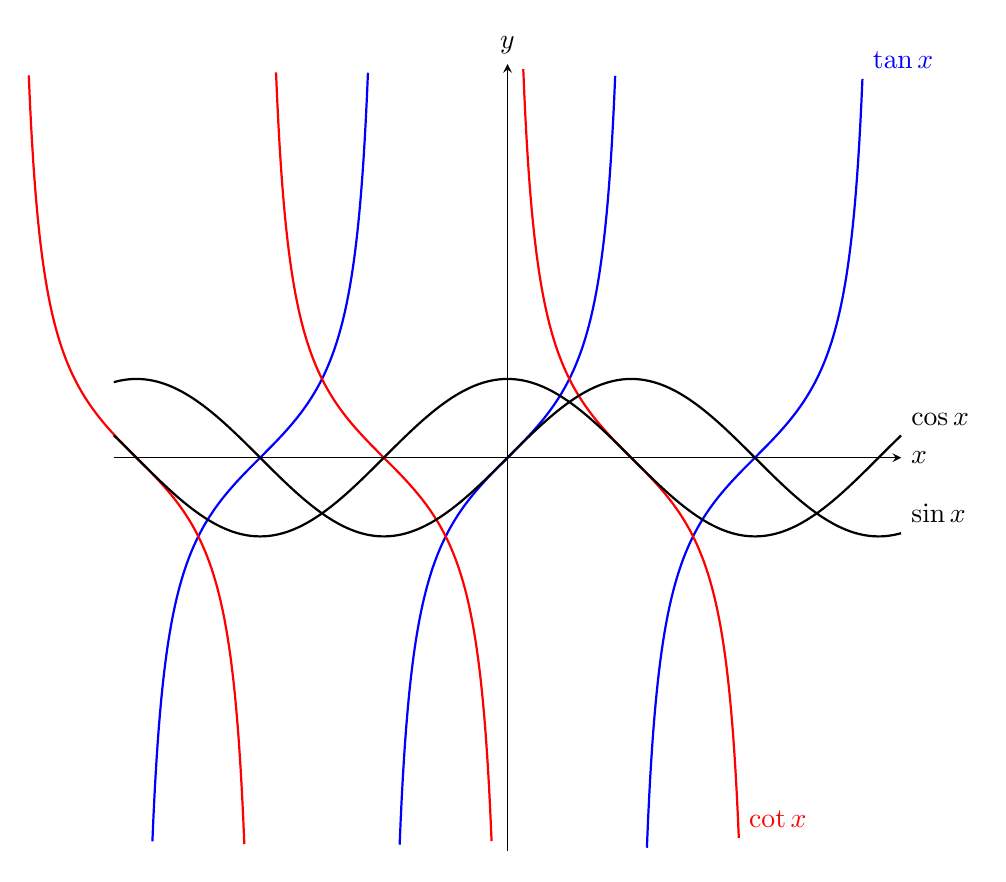
\begin{tikzpicture}
\tzaxes(-5,-5)(5,5){$x$}{$y$}
\tzfn[blue, thick]{tan(\x r)}[(-3.14/2 + 0.2:3.14/2 - 0.2]
\tzfn[blue, thick]{tan(\x r)}[(3.14 -3.14/2 + 0.2:3.14 +3.14/2 - 0.2]{$\tan x$}[ar]
\tzfn[blue, thick]{tan(\x r)}[(-3.14 -3.14/2 + 0.2:-3.14 +3.14/2 - 0.2]

\tzfn[red, thick]{cot(\x r)}[(-3.14 + 0.2: - 0.2]
\tzfn[red, thick]{cot(\x r)}[(3.14 -3.14 + 0.2:3.14 - 0.2]{$\cot x$}[ar]
\tzfn[red, thick]{cot(\x r)}[(-3.14 -3.14 + 0.2:-3.14 - 0.2]

\tzfn[thick]{cos(\x r)}[-5:5]{$\cos x$}[ar]
\tzfn[thick]{sin(\x r)}[-5:5]{$\sin x$}[ar]
\end{tikzpicture}

\subsubsection*{Za vsako kotno funkcijo $f$ (sinus, kosinus, tangens ali kotangens) povejte zvezo med $f(\pi-x)$ in $f(x)$ ter zvezo med $f(\pi+x)$ in $f(x)$ za vsak $x$ iz definicijskega območja funkcije $f$.}

\begin{center}
\begin{tabular}{|c|c|c|}
\hline
 & $f(\pi-x)$ & $f(\pi+x)$ \\
\hline
$\sin x$ & $\sin x=\sin (\pi-x)$ & $\sin x=-\sin (\pi-x)$ \\
\hline
$\cos x$ & $\cos x=-\cos (\pi-x)$ & $\cos x=-\cos (\pi-x)$ \\
\hline
$\tan x$ & $\tan x=-\tan (\pi-x)$ & $\tan x=\tan (\pi-x)$ \\
\hline
$\cot x$ & $\cot x=-\cot (\pi-x)$ & $\cot x=\cot (\pi-x)$ \\
\hline
\end{tabular}
\end{center}

\subsubsection*{Dokažite, da je $\sin \left(\frac{\pi}{2}-x\right)=\cos x$ za vsako realno število $x$.}

\begin{proof}
    $\sin \left(\frac{\pi}{2}-x\right)=\cos x$, ko je $x \in \mathbb{R}$

    $$
\begin{aligned}
& f(x)=\sin \left(\frac{\pi}{2}-x\right)=\sin \frac{\pi}{2} \cdot \cos (-x)+\cos \frac{\pi}{2} \cdot \sin (-x)=1 \cdot \cos (-x)+0 \cdot \\
& \sin (-x)=\cos (-x)=\cos x
\end{aligned}
$$
\end{proof}

\section{Kotne funkcije v pravokotnem trikotniku}
\subsubsection*{Naj bo $\alpha$ ostri kot v danem pravokotnem trikotniku. Definirajte sinus, kosinus, tangens in kotangens kota $\alpha$.}

Sinus ostrega kota $\alpha$ pravokotnega trikotnika je enak razmerju dolžin nasproti ležeče katete in hipotenuze: $\sin \alpha=\frac{a}{c}$

Kosinus ostrega kota $\alpha$ pravokotnega trikotnika je enak razmerju dolžin priležne katete in hipotenuze: $\cos \alpha=\frac{b}{c}$

Tangens ostrega kota $\alpha$ pravokotnega trikotnika je enak razmerju med dolžinama kotu nasproti ležeče katete in kotu priležne katete: $\tan \alpha=\frac{a}{b}$

Kotangens ostrega kota $\alpha$ pravokotnega trikotnika je enak razmerju med dolžinama kotu priležne katete in kotu nasproti ležeče katete: $\cot \alpha=\frac{b}{a}$

\subsubsection*{Naj bo $\alpha$ poljuben kot, $0<\alpha<\frac{\pi}{2}$. Povejte osnovno zvezo med $\sin \alpha$ in $\cos \alpha$ ter jo dokažite.}

Osnovna zveza med $\sin \alpha$ in $\cos \alpha: \sin ^{2} \alpha+\cos ^{2} \alpha=\mathbf{1}($ velja za poljuben kot $\alpha)$

\begin{proof}
    $\sin ^{2} \alpha+\cos ^{2} \alpha=1$

    $a^{2}+b^{2}=c^{2}$

Uporabimo pitagorov izrek.

$\left(\frac{a}{c}\right)^{2}+\left(\frac{b}{c}\right)^{2}=1$

Delimo s $c^{2}$

$\sin ^{2} \alpha+\cos ^{2} \alpha=1$
\end{proof}

\subsubsection*{Povejte še vsaj štiri zveze med kotnimi funkcijami v pravokotnem trikotniku in eno med njimi dokažite.}

\begin{itemize}
\item  $1+\tan ^{2} \alpha=\frac{1}{\cos ^{2} \alpha}$
\item  $1+\cot ^{2} \alpha=\frac{1}{\sin ^{2} \alpha}$
\item  $\tan \alpha=\frac{\sin \alpha}{\cos \alpha}=\frac{1}{\cot \alpha}$
\item $\cot \alpha=\frac{\cos \alpha}{\sin \alpha}$
\end{itemize}

\begin{proof}
    $\tan \alpha=\frac{\sin \alpha}{\cos \alpha}$

    $\tan \alpha=\frac{a}{b}=\frac{\frac{a}{c}}{\frac{b}{c}}=\frac{\sin \alpha}{\cos \alpha}$
\end{proof}
\section{Kotne funkcije}
\subsubsection*{Povejte adicijska izreka za funkciji sinus in kosinus.}

$$
\begin{aligned}
& \sin (\alpha+\beta)=\sin \alpha \cdot \cos \beta+\cos \alpha \cdot \sin \beta \\
& \cos (\alpha+\beta)=\cos \alpha \cdot \cos \beta-\sin \alpha \cdot \sin \beta
\end{aligned}
$$

\subsubsection*{Izrazite $\sin (2 x)$ in $\cos (2 x) \mathrm{s} \sin x$ in $\cos x$. Eno od formul dokažite.}


$\sin 2 \alpha=2 \sin \alpha \cdot \cos \alpha$

$\cos 2 \alpha=\cos ^{2} \alpha-\sin ^{2} \alpha$

\begin{proof}
    $\cos 2 \alpha=\cos ^{2} \alpha-\sin ^{2} \alpha$

    $\cos 2 \alpha=\cos (\alpha+\alpha)=\cos \alpha \cdot \cos \alpha-\sin \alpha \cdot \sin \alpha=\cos ^{2} \alpha-\sin ^{2} \alpha$
\end{proof}

\begin{proof}
    $\sin 2 \alpha=2 \sin \alpha \cdot \cos \beta$

$\sin 2 \alpha=\sin (\alpha+\alpha)=\sin \alpha \cdot \cos \alpha+\sin \alpha \cdot \cos \alpha=2 \sin \alpha \cdot \cos \alpha$
\end{proof}

\subsubsection*{Izrazite $\tan (2 x)$  s $\tan x ?$ Dokažite.}

$\tan 2 \alpha=\frac{2\tan \alpha}{1-\tan^2 \alpha }$

\begin{proof}
    $\tan 2 \alpha=\frac{2\tan \alpha}{1-\tan^2 \alpha }$

$\tan 2 \alpha=\tan (\alpha+\alpha)=\frac{\tan \alpha+\tan \alpha}{1-\tan \alpha \cdot \tan \alpha}=\frac{2 \tan \alpha}{1-\tan ^{2} \alpha}$

$\tan 2 \alpha=\frac{\sin 2 \alpha}{\cos 2 \alpha}=\frac{2 \sin \alpha \cdot \cos \alpha /: \cos ^{2} \alpha}{\cos ^{2} \alpha-\sin ^{2} \alpha /: \cos ^{2} \alpha}=\frac{2 \tan \alpha}{1-\tan ^{2} \alpha}$
\end{proof}

\section{Krožne funkcije}
\subsubsection*{Definirajte funkcijo arkus sinus.}

Funkcija $\arcsin x$ je inverzna funkcija funkciji $\sin x$ na intervalu $x \in [-1, 1]$. Velja torej

$$
\arcsin{\sin{x}} = x
$$

\subsubsection*{Povejte definicijsko območje in zalogo vrednosti funkcije arkus sinus.}

\begin{align*} 
D_f &= [-1, 1] \\
Z_f &= [-\frac{\pi}{2}, \frac{\pi}{2}]
\end{align*}


\subsubsection*{Narišite graf funkcije arkus sinus.}

\begin{center}
  \begin{tikzpicture}
    \begin{axis}[
      axis lines=center,
      xlabel={$x$},
      ylabel={$y$},
      xmin=-1.5,
      xmax=1.5,
      ymin=-2.2,
      ymax=2.2,
      domain=-1:1,
      samples=100
    ]
      \addplot[blue, smooth] {asin(x)/180*pi};
    \end{axis}
  \end{tikzpicture}
\end{center}

\subsubsection*{Definirajte funkcijo arkus tangens.}

Funkcija $\arctan{x}$ je inverzna funkcija funkciji $\tan {x}$ kjer velja:
\begin{align*}
    &x = \tan(y) \land y \in [-\frac{\pi}{2}, \frac{\pi}{2}] \Rightarrow y = \arctan{x}
\end{align*}

\subsubsection*{Narišite graf funkcije arkus tangens.}

\begin{center}
  \begin{tikzpicture}
    \begin{axis}[
      axis lines=center,
      xlabel={$x$},
      ylabel={$y$},
      xmin=-1.5,
      xmax=1.5,
      ymin=-2.2,
      ymax=2.2,
      domain=-1.5:1.5,
      samples=100
    ]
      \addplot[blue, smooth] {atan(x)/180*pi};
    \end{axis}
  \end{tikzpicture}
\end{center}

\section{Krožnica}

\subsubsection*{Povejte geometrijsko definicijo krožnice in izpeljite enačbo krožnice s polmerom $r$ in s središčem v točki $S(p, q)$.}

Krožnica je množica točk v ravnini, ki so enako oddaljene od izbrane točke. Izbrana točka je središče ($S$). Oddaljenost je polmer ($r$).

\vspace{5mm}

Enačba krožnice s polmerom $r$ in središčem v točki $S(p, q)$:

$$
(x-p)^2 + (y-q)^2 = r^2
$$

\vspace{5mm}

Izpeljava enačbe:

\begin{equation*}
\begin{gathered}
S(p, q) \\
T(x, y) \\
\\
d(S, T) = r \\
\sqrt{(x-p)^2 + (y-q)^2} = r \\
(x-p)^2 + (y-q)^2 = r^2
\end{gathered}
\end{equation*}

\subsubsection*{Naj bodo $A$, $D$, $E$ in $F$ realna števila in naj bo $A \neq 0$. Katere množice točk v ravnini lahko predstavlja enačba $A x^{2}+A y^{2}+D x+E y+F=0$?}

Enačba lahko predstavlja:

\begin{itemize}
  \item Točko
  \item Krožnico
  \item Prazno množico
\end{itemize}

\subsubsection*{Analizirajte, za katera realna števila $a$ in $b$ enačba $x^{2}+y^{2}+2 a x+2 b y+4=0$ predstavlja krožnico.}

\begin{equation*}
\begin{gathered}
x^2 + y^2 + 2ax + 2by + 4 = 0 \\
(x+a)^2 - a^2 + (y+b)^2 - b^2 + 4 = 0 \\
(x+a)^2 + (y+b)^2 = a^2 + b^2 - 4
\end{gathered}
\end{equation*}

\vspace{5mm}

Enačba predstavlja krožnico, ko je:

$$
a^2 + b^2 - 4 > 0
$$

\section{Elipsa}

\subsubsection*{Povejte geometrijsko definicijo elipse.}

Elipsa je množica točk v ravnini, za katere je vsota razdalj do dveh izbranih točk konstantna. Izbrani točki sta gorišči.

\vspace{5mm}

Naj bosta $F_1$ in $F_2$ gorišči. Potem je $d(T, F_1) + d(T, F_2) = konst$. Ta konstanta je dvakratnik daljše polosi elipse.

\subsubsection*{Povejte enačbo elipse s središčem v koordinatnem izhodišču in enačbo elipse s središčem v točki $S(p, q)$. V obeh primerih naj bosta osi elipse vzporedni koordinatnima osema.}

Središče v koordinatnem izhodišču:

$$
\frac{x^2}{a^2} + \frac{y^2}{b^2} = 1
$$

Središče v $S(p, q)$:
$$
\frac{(x-p)^2}{a^2} + \frac{(y-q)^2}{b^2} = 1
$$

\subsubsection*{Naj bodo $A$, $C$, $D$, $E$ in $F$ realna števila in naj bo $A \cdot C>0$. Katere množice točk v ravnini lahko predstavlja enačba $A x^{2}+C y^{2}+D x+E y+F=0$?}

Enačba lahko predstavlja:

\begin{itemize}
  \item Točko
  \item Krožnico
  \item Elipso
  \item Prazno množico
\end{itemize}

\section{Hiperbola}

\subsubsection*{Povejte geometrijsko definicijo hiperbole.}

Hiperbola je množica točk v ravnini, za katere je absolutna vrednost razlike razdalj do dveh izbranih točk konstantna. Izbrani točki sta gorišči.

\vspace{5mm}

Naj bosta $F_1$ in $F_2$ gorišči. Potem je $|d(T, F_1) - d(T, F_2)| = konst$. Ta konstanta je dvakratnik realne polosi hiprebole.

\subsubsection*{Povejte enačbo hiperbole s središčem v koordinatnem izhodišču in enačbo hiperbole s središčem v točki $S(p, q)$. V obeh primerih naj bosta osi hiperbole vzporedni koordinatnima osema.}

Središče v koordinatnem izhodišču:

$$
\frac{x^2}{a^2} - \frac{y^2}{b^2} = \pm 1
$$

Središče v $S(p, q)$:
$$
\frac{(x-p)^2}{a^2} - \frac{(y-q)^2}{b^2} = \pm 1
$$

\subsubsection*{Naj bodo $A$, $C$, $D$, $E$ in $F$ realna števila in naj bo $A \cdot C<0$. Katere množice točk v ravnini lahko predstavlja enačba $A x^{2}+C y^{2}+D x+E y+F=0$?}

Enačba lahko predstavlja:

\begin{itemize}
    \item Hiperbolo
    \item Dve sekajoči se premici
\end{itemize}

\section{Parabola}

\subsubsection*{Povejte geometrijsko definicijo parabole.}

Parabola je množica točk v ravnini, ki so enako oddaljene od premice in točke, ki ne leži na premici. Izbrana točka je gorišče, premica pa vodnica.

\subsubsection*{Povejte enačbo parabole, ki ima teme v točki $T(r, d)$, njena os simetrije pa je vzporedna abscisni osi. Izračunajte gorišče in enačbo premice vodnice te parabole.}

$$
(y-d)^2 = 2p(x-r)
$$

\vspace{5mm}

\centerline{Gorišče: $F(r + \frac{p}{2}, d)$} 
\vspace{2mm}
\centerline{Vodnica: $x = r - \frac{p}{2}$}

\subsubsection*{Naj bodo $A$, $C$, $D$, $E$ in $F$ realna števila in naj bo $A=0$ in $C \neq 0$ ali $C=0$ in $A \neq 0$. Katere množice točk v ravnini lahko predstavlja enačba $A x^{2}+C y^{2}+D x+E y+F=0$?}

Enačba lahko predstavlja:

\begin{itemize}
  \item Parabolo
  \item Eno premico
  \item Dve vzporedni premici
  \item Prazno množico
\end{itemize}

\section{Zaporedja}

\subsubsection*{Definirajte zaporedje. Kaj je graf zaporedja?}

ZAPOREDJE realnih števil je funckija, ki vsakemu naravnemu številu $n$ priredi neko realno število $a_{n}$ :
$$
f: \mathbb{N} \rightarrow \mathbb{R}, f: n \mapsto a_{n} \text{ ali } f(n)=a_{n}
$$

Graf zaporedja so točke v koordinatnem sistemu, katerih abscisa je $n$, ordinata pa $a_{n}$ : $T\left(n, a_{n}\right)$

\subsubsection*{Kdaj je zaporedje monotono in kdaj omejeno?}

Zaporedje je MONOTONO, ko je ali naraščajoče ali padajoče.

Pravimo, da je zaporedje padajoče, če za vsako naravno število $n$ velja $a_{n+1} \leq a_{n}$, in da je strogo padajoče, če velja $a_{n+1}<a_{n}$.

Pravimo, da je zaporedje naraščajoče, če za vsako naravno število $n$ velja $a_{n+1} \geq a_{n}$, in da je strogo padajoče, če velja $a_{n+1}>a_{n}$.

Zaporedje je OMEJENO, ko je navzgor in navzdol omejeno.

Zaporedje je navzgor omejeno, če obstaja atako število $M$, da je $a_{n} \leq M$ za vsako naravno število n. Najmanjša zgornja meja je supremum ali natančna zgornja meja. Zaporedje je navzdol omejeno, če obstaja atako število $m$, da je $a_{n} \geq m$ za vsako naravno število n. Največja spodnja meja je infimum ali natančna spodnja meja.

\subsubsection*{Kdaj je zaporedje konvergentno in kdaj divergentno?}

Zaporedje je KONVERGENTNO, ko ima limito, in DIVERGENTNO, ko limite nima.

\subsubsection*{Povejte primer konvergentnega in primer divergentnega zaporedja.}
Zaporedje je KONVERGENTNO, ko ima limito, in DIVERGENTNO, ko limite nima.
\begin{itemize}
  \item PRIMER konvergentnega zaporedja:

\end{itemize}

\begin{align*}
    a_{n}&=\frac{1}{n} \\
    a_{1}&=\frac{1}{1}=1, a_{2}=\frac{1}{2}, a_{3}=\frac{1}{3} \ldots
\end{align*}
Zaporedje se približuje številu 0 , kar je limita zaporedja.

\begin{itemize}
  \item PRIMER divergentnega zaporedja:
\end{itemize}

$a_{n}=2^{n}$

$a_{1}=2, a_{2}=4, a_{3}=8 \ldots$

Zaporedje gre v neskončnost, nima limite.


\section{Aritmetično zaporedje}
\subsubsection*{Definirajte aritmetično zaporedje in povejte njegov splošni člen.}

Zaporedje je \textit{aritmetično}, če je razlika med dvema zaporednima členoma enaka:
$$
a_{n+1} - a_n = d
$$
kjer je $d$ konstanta.
\subsubsection*{Podajte primer padajočega aritmetičnega zaporedja.}

18, 14, 10, 6, ... $d=-4$

\subsubsection*{Kako izračunamo vsoto prvih $n$ členov aritmetičnega zaporedja, če poznamo prvi člen in diferenco? Trditev dokažite.}

Uporabimo enačbo:
$$
S_n = \frac{n}{2}(2a_1 + (n-1)d)
$$

\begin{proof}
    Osnovi korak (n=1):
    $$
        a_1 = \frac{1}{2}(2\cdot a_1 + 0\cdot d) 
    $$
    Indukcijski korak $n \rightarrow n + 1$:
    \begin{gather*}
        \frac{n}{2}(2a_1 + (n-1)d) + a_1 + n \cdot d = \frac{1}{2} \cdot (2a_1\cdot n + n(n-1)d + 2a_1 + 2n \cdot d) = \\
        \frac{1}{2} \cdot (2a_1(n+1) + nd(n-1 + 2)) = \frac{n+1}{2}(2a_1 + n \cdot d)
    \end{gather*}
\end{proof}
\subsubsection*{Dokažite, da je zaporedje $\left(a_{k}\right)$ aritmetično natanko tedaj, ko je za poljubno naravno število $n$ aritmetična sredina členov $a_{n}$ in $a_{n+2}$ enaka $a_{n+1}$.}

\begin{proof}
    \begin{gather}
        a_n = a_1 + (n-1)d \\
        a_{n-1} = a_1 + (n-2)d \\
        a_{n+1} = a_1 + nd \\
        a_{n-1} + a_{n+1} = 2a_1 + 2nd - 2d = 2(a_1+(n-1)d) = 2a_n
    \end{gather}
\end{proof}

\section{Geometrijsko zaporedje}
\subsubsection*{Definirajte geometrijsko zaporedje in povejte njegov splošni člen.}

Zaporedje je geometrijsko, če je kvocient med dvema zaporednima členoma konstanten.
$$
\frac{a_{n+1}}{a_n} = k
$$
kjer je $k$ konstanta.
\subsubsection*{Kako izračunamo vsoto prvih $n$ členov geometrijskega zaporedja, če poznamo prvi člen in količnik? Kako izračunamo to vsoto, če je količnik enak 1? Trditvi dokažite.}

V splošnem uporabimo enačbo:
$$
S_n = \frac{a_1(k^n - 1)}{k-1}
$$

\begin{proof}
    Osnovi korak (n=1):
    $$
        a_1 = \frac{a_1 \cancel{(k^1 - 1)}}{ \cancel{k-1}} = a_1
    $$
    Indukcijski korak $n \rightarrow n + 1$:
    \begin{gather*}
        S_n = \frac{a_1(k^n - 1)}{k-1} + a_1 \cdot k^n =
        \frac{a_1(k^n-1) + a_1 \cdot k^n \cdot (k-1)}{k-1} = \\
        \frac{\cancel{a_1 k^n} - a_1 + a_1 k^{n+1} - \cancel{a_1 k^n}}{k-1} =
        \frac{a_1(k^{n+1} - 1)}{k-1}
    \end{gather*}
\end{proof}


Če je količnik enak 1, potem:

$$
S_n = n\cdot a_1
$$

\begin{proof}
    $$
    a_n = a_1\cdot 1^n = a_1
    $$
    Iz tega sledi da:
    $$
    S_n = a_1 + a_2 \dots a_{n-1} + a_n = a_1 + a_1 \dots a_1 + a_1 = n \cdot a_1
    $$
\end{proof}
\subsubsection*{Naj bo ( $a_{k}$ ) zaporedje s pozitivnimi členi. Dokažite, da je $\left(a_{k}\right)$ geometrijsko zaporedje natanko tedaj, ko je za poljubno naravno število $n$ geometrijska sredina členov $a_{n}$ in $a_{n+2}$ enaka $a_{n+1}$.}

\begin{proof}
    \begin{gather}
        a_n = a_1 \cdot k^{n-1} \\
        a_{n-1} = a_1 \cdot k^{n-2} \\
        a_{n+1} = a_1  \cdot k^{n} \\
        a_{n-1} \cdot a_{n+1} = {a_1}^2 k^{2n-2} = {a_n}^2
    \end{gather}
\end{proof}

\section{Geometrijska vrsta}
\subsubsection*{Kaj je vrsta? Kdaj je vrsta konvergentna in kdaj divergentna? Kaj je vsota konvergentne vrste?}

VRSTA je vsota členov nekega zaporedja. Vrsta $a_{1}+a_{2}+\cdots+a_{n}+\cdots$ je konvergentna, če je konvergentno zaporedje delnih vsot $S_{1}, S_{2}, S_{3}, \ldots, S_{n}, \ldots$ Delne vsote so vsote nekaj začetnih členov:

$S_{1}=a_{1}, S_{2}=a_{1}+a_{2}, S_{n}=a_{1}+a_{2}+a_{3}+\ldots+a_{n}$. To pomeni, da lahko seštejemo neskončno število členov zaporedja. Vrsta je divergentna, če zaporedje delnih vsot ni konvergentno. To pomeni, da ne moremo sešteti neskončno število členov zaporedja.



\subsubsection*{Definirajte geometrijsko vrsto. Kako ugotovimo, ali je geometrijska vrsta konvergentna?}

Vsota členov geometrijskega zaporedja se imenuje GEOMETRIJSKA VRSTA. Neskončna geometrijska vrsta je konvergentna, če obstaja limita delnih vsot. $S_{x}=\lim _{n \rightarrow \infty} S_{n}$ $S_{x}=\lim _{\mathrm{n} \rightarrow \infty} \frac{a_{1}\left(\mathrm{k}^{\mathrm{n}}-1\right)}{(\mathrm{k}-1)}$


\subsubsection*{Kako izračunamo vsoto konvergentne geometrijske vrste, če poznamo prvi člen in količnik? Trditev dokažite.}

Vsoto konvergentne geometrijske vrste s količnikom $k$ izračunamo po formuli:

$$
S=\frac{a_{1}}{k-1} \cdot \lim _{\mathrm{n} \rightarrow \infty}\left(\mathrm{k}^{\mathrm{n}}-1\right)=\frac{a_{1}}{\mathrm{k}-1} \cdot(-1)=\frac{a_{1}}{1-\mathrm{k}}
$$

\section{\texorpdfstring{\cancel{Obrestni račun}}{Obrestni račun}}
\subsubsection*{Opišite osnovne pojme obrestno obrestnega računa: glavnica, obresti, obrestovalni faktor, kapitalizacijsko obdobje.}

\begin{itemize}
    \item Glavnica - vrednost, ki se obrestuje
    \item Obrest - znesek, za katerega se glavnica povečuje
    \item Obrestovalni faktor - faktor s katerim množimo glavnico da dobimo glavnico po obrestovanju $(1+p)$
    \item Kapitalizacijsko obdobje - Čas za katerega se računajo obresti in se ob preteku tega obdobja pripišejo glavnici
\end{itemize}

\subsubsection*{Opišite primer varčevanja na banki, ki uporablja obrestno obrestovanje z letnim pripisom obresti. Kako izračunamo višino privarčevanega zneska?}

Recimo da na banko položimo 1000 eur in je obrestna mera 5\%. Potem je nova glavnica po prvem letu enaka 1000eur + $0.05 \cdot 1000$ oz skupaj 1050 eur. Naslednje leto je glavnica 1050 eur, ki ji nato spet prištejemo obrest. V splošnem je tako privarčevan znesek enak:

$$
G_n = G_0 \cdot r^n
$$
kjer je $r$ obrestovalni faktor in $n$ število let varčevanja.

\subsubsection*{Opišite primer obročnega odplačevanja posojila na banki, ki uporablja obrestno obrestovanje z letnim pripisom obresti. Kako izračunamo višino obroka?}

Recimo da si od banke izposodimo 1000 eur in ga bomo vrnili v 10 letih po 0.05 obrestni meri. Potem moramo vse skupaj vrniti $1000 \cdot (1+0.05)^10$. Recimo da odplačujemo kredit mesečno. Torej je velikost obroka v splošnem:
$$
O = \frac{G_0 \cdot r^n}{12n}
$$
\section{Odvod}
\subsubsection*{Definirajte odvod funkcije v dani točki in opišite njegov geometrijski pomen.}

Odvod funkcije v dani točki je enak limiti diferenčnega količnika, ko gre sprememba neodvisne spremenljivke proti 0 , torej $f(x)=\lim _{n \rightarrow 0} \frac{f(x+h)-f(x)}{h}$. Odvod funkcije v dani točki je enak smernemu koeficientu tangetne na graf funkcije v tej točki.

\subsubsection*{Podajte primer funkcije in točke, v kateri je funkcija odvedljiva, in po definiciji odvoda izračunajte njen odvod v izbrani točki.}

PRIMER:

Naj bo funckija f funkcija s predpisom $f(x)=x^{2}$ in točka $T(3,9)$ točka na njenem grafu.

Odvod funkcije $f v$ točki T je enak:

$$
f^{\prime}(3)=\lim _{n \rightarrow 0} \frac{f(3+h)-f(3)}{h}=\lim _{n \rightarrow 0} \frac{9+6 h+h^{2}-9}{h}=\lim _{n \rightarrow 0}(6+h)=6
$$
\subsubsection*{Naj bo funkcija $f$ odvedljiva v točki $x_{0}$. Kako izračunamo enačbo tangente na graf funkcije $f$ v točki $x_{0}$ ?}

Najprej poiščemo odvod funkcije $f v$ točki $T\left(x_{0}, y_{0}\right)$, nato pa zapišemo enačbo TANGENTE $y=\mathrm{f}^{\prime}\left(x_{0}\right) x+\mathrm{n}$ ter vanjo vstavimo dano točko in izračunamo $\mathrm{n}$ : $\mathrm{n}=y_{0}-\mathrm{f}^{\prime}\left(x_{0}\right) x_{0}$. Zapišemo enačbo tangente v obliki: $y=\mathrm{f}^{\prime}\left(x_{0}\right) x+\mathrm{n}$

\subsubsection*{Naj bo funkcija $f$ odvedljiva v točki $x_{0}$ in naj bo $f^{\prime}\left(x_{0}\right) \neq 0$. Kako izračunamo enačbo normale na graf funkcije $f v$ točki $x_{0}$ ?}

Enačbo NORMALE izračunamo tako, da najprej poiščemo odvod funkcije $f$ v točki $T\left(x_{0}, y_{0}\right)$,nato pa zapišemo enačbo $\mathrm{y}=-\frac{1}{\mathrm{f}^{\prime}\left(\mathrm{x}_{0}\right)} \mathrm{x}+\mathrm{n}$ ter vanjo vstavimo dano točko in izračunamo $\mathrm{n}: \mathrm{n}=\mathrm{y}_{0}+\frac{1}{\mathrm{f}^{\prime}\left(\mathrm{x}_{0}\right)} \mathrm{x}_{0}$.


\section{Lokalni ekstremi}
\subsubsection*{Definirajte lokalni maksimum in lokalni minimum funkcije.}

Funkcija f ima v točki $x=$ a lokalni maksimum natanko tedaj, ko obtaja takšna okolica števila a $O_{\varepsilon}(a)$, da za vsak $x \in O_{\varepsilon}(a)$ velja: $f(x) \leq f(a)$.

Funkcija f ima v točki $x=$ a lokalni minimum natanko tedaj, ko obtaja takšna okolica števila a $O_{\varepsilon}(a)$, da za vsak $x \in O_{\varepsilon}(a)$ velja: $f(x) \geq f(a)$.

\subsubsection*{Naj bo $f: \mathbb{R} \rightarrow \mathbb{R}$ odvedljiva funkcija. Kako s pomočjo prvega odvoda ugotovimo, ali ima funkcija $f$ v točki $x_{0}$ lokalni ekstrem?}
 Funkcija f ima v točki xo lokalni ekstrem natanko tedaj, ko je prvi odvod funkcije v tej točki enak 0 , prva odvoda v točkah $x_{0}-\varepsilon$ in $x_{0}+\varepsilon ; \varepsilon \rightarrow 0$ pa imata različna predznaka.


\subsubsection*{Naj bo $f: \mathbb{R} \rightarrow \mathbb{R}$ dvakrat odvedljiva funkcija in $x_{0}$ njena stacionarna točka. Kako s pomočjo drugega odvoda ugotovimo, ali ima funkcija $f$ v točki $x_{0}$ lokalni ekstrem?}

Funkcija f ima v stacionarni točki xo lokalni ekstrem natanko tedaj, ko je drugi odvod funkcije v tej točki različen od 0 .

\section{\texorpdfstring{\cancel{Ekstremi}}{Ekstremi}}
\subsubsection*{Definirajte globalni maksimum in globalni minimum funkcije.}



\subsubsection*{Opišite postopek za iskanje globalnih ekstremov odvedljive funkcije, definirane na zaprtem intervalu.}



\subsubsection*{Povejte primer funkcije, katere globalni minimum je enak njenemu globalnemu maksimumu.}



\subsubsection*{Povejte primer omejene funkcije, ki nima globalnega maksimuma.}



\section{Odvod}
\subsubsection*{Naj graf odvedljive funkcije $f$ seka abscisno os v točki $T\left(x_{0}, 0\right)$. Povejte definicijo kota $\alpha$ med grafom funkcije $f$ in abscisno osjo v točki $T$. Kako izračunamo kot $\alpha$, če poznamo $f^{\prime}\left(x_{0}\right)$ ?}

Kot $\alpha$ med grafom funkcije f in abscisno osjo v točki $\mathrm{T}\left(x_{0}, 0\right)$, je kot med tangentno na graf funkcije v točki T in poltrakom v pozitivni smeri abscisne osi, merjen od poltraka v pozitivni smeri.

Če poznamo $f^{\prime}\left(x_{0}\right)$ ga za $f^{\prime}\left(x_{0}\right) \geq 0$ izračunamo po formuli $\alpha=\arctan f^{\prime}\left(x_{0}\right)$ in za $f^{\prime}\left(x_{0}\right) \geq 0$ po formuli $=\pi+\arctan f^{\prime}\left(x_{0}\right)$.

\subsubsection*{Naj graf odvedljive funkcije $f$ seka ordinatno os v točki $T\left(0, y_{0}\right)$. Povejte definicijo kota $\beta$ med grafom funkcije $f$ in ordinatno osjo v točki $T$. Kako izračunamo kot $\beta$, če poznamo $f^{\prime}(0) ?$}

Kot $\beta$ med grafom funkcije f in ordinatno osjo $\mathrm{v}$ točki T(0, yo) je manjši izmed obeh kotov, pod katerima se sekata tangenta na graf funkcije $f v$ točki $T$ in ordinatna os. Če poznamo $f^{\prime}(0)$ ga izračunamo po formuli $\beta=90^{\circ}-\arctan \left|f^{\prime}(0)\right|$.



\subsubsection*{Naj se grafa odvedljivih funkcij $f$ in $g$ sekata v točki $T\left(x_{0}, y_{0}\right)$. Povejte definicijo kota $\varphi$ med grafoma funkcij $f$ in $g$ točki $T$. Kako izračunamo kot $\varphi$, če poznamo $f^{\prime}\left(x_{0}\right)$ in $g^{\prime}\left(x_{0}\right)$ (pri tem upoštevajte vse možne situacije)?}

$\quad \operatorname{Kot} \varphi$ med grafoma funkcij $f$ in $g$ v točki $T$ je manjši izmed obeh kotov, pod katerima se sekata tangetni na grafa $f$ in $g$ v točki T.

Če poznamo $f^{\prime}\left(x_{0}\right)$ in $g^{\prime}\left(x_{0}\right)$, ga izračunamo po formuli $\varphi=\arctan \left|\frac{f^{\prime}\left(x_{0}\right)-g^{\prime}\left(x_{0}\right)}{1+f^{\prime}\left(x_{0}\right) \cdot g^{\prime}\left(x_{0}\right)}\right|$. Če je $1+f^{\prime}\left(x_{0}\right) \cdot g^{\prime}\left(x_{0}\right)=0$, se grafa sekata pod pravim kotom $\varphi=90^{\circ}$.

\section{Nedoločeni integral}
\subsubsection*{Definirajte nedoločeni integral funkcije.}

NEDOLOČENI INTEGRAL funkcije je družina funkcij, ki so določene le do konstante natančno in so inverzne funkciji diferenciranja.

\subsubsection*{Povejte pravili za integriranje vsote funkcij in za integriranje produkta funkcije s konstanto.}

Pravila za integriranje funkcije:

\begin{enumerate}
  \item integriranje vsote funkcij
  $\int(f(x)+g(x)) d x=\int f(x) d x+\int g(x) d x$
  \item integriranje produkta funkcije s konstantno
  $\int a f(x) d x=a \int f(x) d x$
\end{enumerate}

\subsubsection*{Na primeru opišite metodo uvedbe nove integracijske spremenljivke pri računanju nedoločenega integrala.}

Poiščemo nedoločeni integral $\int \frac{1}{3 x+2} d x$. Za novo spremenljivko vzamemo $t=3 x+2$ in enačbo diferenciramo. Dobimo $d t=3 d x$. Izrazimo $\mathrm{dx}$, torej $d x=\frac{d t}{3}$, in zapišemo $\int \frac{1}{t} \cdot \frac{d t}{3}=\frac{1}{3} \ln |t|+c=\frac{1}{3} \ln |3 x-2|+c$

\section{Nedoločeni integral}
\subsubsection*{Naj bo a poljubno pozitivno realno število in naj bo $r$ poljubno realno število.}

\subsubsection*{Izračunajte $\int x^{r} d x$ (tako za $r \neq-1$ kot za $r=-1$ ).}

$$
\begin{aligned}
& \int x^{r} d x ; r \in \mathbb{R}, r \neq-1: \int x^{r} d x=\frac{1}{r+1} x^{r+1}+c \\
& \int x^{r} d x ; r \in \mathbb{R}, r=-1: \int x^{r} d x=\ln |x|+c \\
\end{aligned}
$$


\subsubsection*{Izračunajte $\int a^{x} \mathrm{~d} x$}

$$
\int a^{x} d x ; a \in \mathbb{R}^{+}: \int a^{x} d x=\frac{a^{x}}{\ln a}+c
$$

\subsubsection*{Povejte formulo za integracijo z metodo integracije po delih (per partes).}

$\int u d v=u \cdot v-\int v d u$

\subsubsection*{Metodo integracije po delih razložite na primeru.}

Poiščemo nedoločeni integral $\int x \cdot e^{x} d x$. Naj bo $u=x$ in $d v=e^{x} d x$.

Potem je $d u=d x$ in $v=e^{x}$. Po formuli za integracijo z metodo integracije po delih zapišemo: $\int x \cdot e^{x} d x=x \cdot e^{x}-\int e^{x} d x=x \cdot e^{x}-e^{x}+c=e^{x}(x-1)+c$.

\section{Določeni integral}
\subsubsection*{Skicirajte lik, ki ga na intervalu $[a, b]$ omejujejo graf zvezne pozitivne funkcije $f$, abscisna os ter premici $x=a$ in $x=b$. Kako izračunamo ploščino tega krivočrtnega lika?}

Skica lika, ki ga na intervalu [a, b] omejujejo graf zvezve pozitivne funkcije $f$, abscisna od ter premici $x=a$ in $x=b$ :
\begin{center}
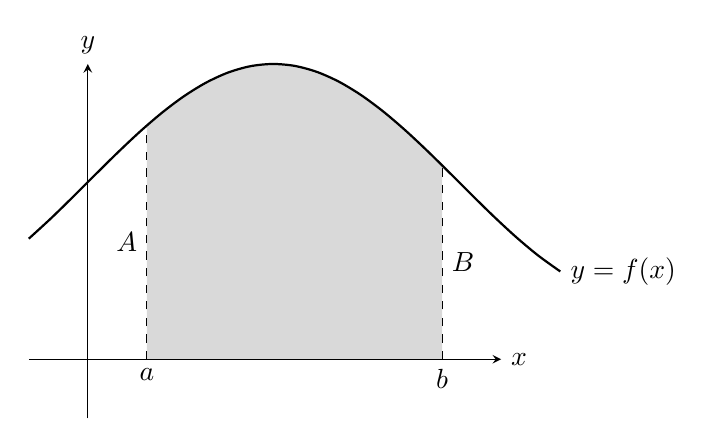
\begin{tikzpicture}[scale=1.5]
  % Area under the curve
  \fill[gray!30] (0.5,0) -- plot [domain=0.5:3, smooth, variable=\x] (\x,{sin(\x r)+1.5}) -- (3,0) -- cycle;
  
  \draw[->] (-0.5,0) -- (3.5,0) node[right] {$x$};
  \draw[->] (0,-0.5) -- (0,2.5) node[above] {$y$};

  % Curve
  \draw[thick, domain=-0.5:4, smooth, variable=\x] plot (\x,{sin(\x r)+1.5}) node[right] {$y=f(x)$};
 
  % Points A and B
  \coordinate (A) at (0.5,0);
  \coordinate (B) at (3,0);
  
  % Vertical lines and labels for A and B
  \draw[dashed] (A) -- ++(0,1.5+0.479) node[pos=0.5, left] {$A$};
  \draw[dashed] (B) -- ++(0,1.5+0.14) node[pos=0.5, right] {$B$};

  % Axes labels
  \node[below] at (A) {$a$};
  \node[below] at (B) {$b$};
\end{tikzpicture}
\end{center}
Ploščino lika izračunamo z določenim integralom: $S=\left|\int_{a}^{b} f(x) d x \right|$

\subsubsection*{Naj bo $f: \mathbb{R} \rightarrow \mathbb{R}$ liha zvezna funkcija in a pozitivno realno število. Koliko je $\int_{-a}^{a} f(x) d x ?$ Utemeljite odgovor.}

Določeni integral $\int_{-a}^{a} f(x) d x$ je enak vsoti integralov $\int_{-a}^{0} f(x) d x$ in $\int_{0}^{a} f(x) d x$. Ker je liha, vemo, da je simetrična glede na koordinatno izhodišče, torej sta ploščina lika, ki ga omejujejo krivulja abscisa in premica $x=-a$, in ploščina lika, ki ga omejujejo krivulja, abscisa in premica $x=a$, enaki.

Iz tega sledi, da sta tudi integrala $\int_{-a}^{0} f(x) d x$ in $\int_{0}^{a} f(x) d x$ po absolutni vrednosti enaka. Ker je funkcija simetrična glede na koordinatno izhodišče, vemo tudi, da eden izmed likov leži nad abscisno osjo, drugi pa pod njo, torej je eden izmed integralov $\int_{-a}^{0} f(x) d x$ in $\int_{0}^{a} f(x) d x$ pozitiven, drug pa negativen. Iz tega sledi, da sta si integrala $\int_{-a}^{0} f(x) d x$ in $\int_{0}^{a} f(x) d x$ nasprotna, njuna vsota pa je zato enaka 0.

\subsubsection*{Krivočrtni lik, ki ga z abscisno osjo na intervalu $[a, b]$ določa graf zvezne pozitivne funkcije $f$, zavrtimo okoli abscisne osi za $360^{\circ}$. Narišite skico. Povejte formulo za prostornino nastalega rotacijskega telesa.}
Prostornina nastalega telesa je:
$$
V = \pi \int_{a}^{b}{f^2(x) dx}
$$

\textit{Skica je prepuščena kot naloga bralcu.}
\section{Določeni integral}
\subsubsection*{Naj bo $f:[a, b] \rightarrow \mathbb{R}$ zvezna funkcija. Pojasnite geometrijski pomen določenega integrala funkcije $f$ na intervalu $[a, b]$.}

Če je funkcija f na intervalu $[a, b]$ :

\begin{itemize}
  \item pozitivna, je določeni integral funkcije na tem intervalu enak ploščini lika, ki ga omejujejo krivulja, abscisna os in premici $x=a$ in $x=b$.

  \item negativna, je določeni integral funkcije na tem intervalu enak nasprotni vrednosti ploščine lika, ki ga omejujejo krivulja, abscisna os in premici $x=a$ in $x=b$.

\end{itemize}

V splošnem je določeni integral neke funckije na intervalu $[a, b]$ enak razliki ploščin likov nad abscisno osjo in likov pod njo, ki jih na intervalu [a, b] omejujeta krivulja in abscisna os oziroma krivulja abscisna os ter premica $x=a$ ali premica $x=b$.

\subsubsection*{Povejte zvezo med določenim in nedoločenim integralom (Newton-Leibnizeva formula). Navedite primer.}

Določeni integral funkcije $f$ na intervalu $[a, b]$ je enak razliki vrednosti nedoločenega integrala funkcije $f v$ točkah $x=b$ in $x=a$, torej:

$$\int_{a}^{b} f(x) d x=F(b)-F(a) ; F(x)=\int f(x) d x$$

\textbf{PRIMER:}

$f(x)=x \quad F(x)=\frac{1}{2} x^{2}$

$\int_{1}^{2} x d x=\frac{1}{2} 2^{2}-\frac{1}{2} 1^{2}=\frac{3}{2}$

\subsubsection*{Na primeru razložite metodo uvedbe nove spremenljivke pri računanju določenega integrala.}

Izračunamo določeni integral $\int_{1}^{4} \frac{e^{\sqrt{x}}}{\sqrt{x}} d x$. Uvesti moramo novo spremenljivko $t=\sqrt{x}$, enačbo diferencirati $\left(d t=\frac{1}{2} \cdot \frac{1}{\sqrt{x}} d x\right)$ in poiskati nove meje določenega integrala $\left(t_{1}=\sqrt{1}=1\right.$ in $\left.t_{2}=\sqrt{4}=2\right)$. Zapišemo $\int_{1}^{2} \frac{e^{t}}{t} 2 d t$ in izračunamo integral $\int_{1}^{4} \frac{e^{\sqrt{x}}}{\sqrt{x}} d x=\int_{1}^{2} \frac{e^{t}}{t} 2 t d t=2 \int_{1}^{2} e^{t} d t=2 e^{2}-2 e=2 e(e-1)$

\section{\texorpdfstring{\cancel{Kombinatorika}}{Kombinatorika}}
\subsubsection*{Povejte osnovni izrek kombinatorike.}

Naj bo proces izbiranja takšen, da poteka v k zaporednih fazah. V prvi fazi izbiramo med $n_{1}$ možnostmi, v drugi fazi med $n_{2}$ možnostmi, ... in $v \mathrm{k}$-ti fazi med $n_{k}$ možnostmi, vsakokrat neodvisno od tega, katere možnosti smso izbrali v predhodnih fazah.

Potem je mogoče sestavljeni izbor opraviti na natanko $\mathrm{N}=\mathrm{n}_{1} \cdot \mathrm{n}_{2} \cdot \ldots \cdot \mathrm{n}_{\mathrm{k}}$ načinov.

\subsubsection*{Uporabo osnovnega izreka kombinatorike razložite na primeru}

Janez ima na voljo dva para čevljev, 3 različne puloverje in zelene ter modre hlače. Na

koliko načinov se Janez lahko obleče, če bo oblekel ene čevlje, ene hlače in en pulover?

2 Č $\rightarrow 3 \mathrm{P} \rightarrow 2 \mathrm{H}---12$ različnih opcij ima

\subsubsection*{Povejte pravilo vsote.}

Če se pri izbiranju odločamao med $\mathrm{n}_{1}$ možnostmi iz prvega izbora ali med $\mathrm{n}_{2}$ možnostmi iz drugega izbora ali ... med $n_{k}$ možnostmi iz k-tega izbora, je vseh možnih izborov: $\mathrm{N}=\mathrm{n}_{1}+\mathrm{n}_{2}+\cdots+\mathrm{n}_{\mathrm{k}}$

\subsubsection*{Uporabo pravila vsote razložite na primeru.}

Na kavomatu lahko dobimo 5 vrst kave, 3 vrste kapučina in 2 vrsti čaja. Napitek lahko naročimo z žličko ali brez. Na koliko načinov lahko dobimo seriviran napitek iz avtomata?

Kombinatorično drevo - veje so posamezne faze:

$3-5$

3

5

5+3+2 opcij krat 2, saj lahko naročimo z žličko ali brez. Torej je vseh opcij 20.

\subsubsection*{Povejte pravilo vključitev in izključitev za dve množici ter ga razložite na primeru.}

Pravilo vključitev in izključitev je posplošitev pravila vsote. Pri izbiranju iz več množic moramo paziti, da je vsak element upoštevan natanko enkrat. Ko torej izbiramo med elementi ene ali druge množice in njun presek ni prazen, dobimo število elementov tako:

$$
m(a \cup b)=m(a)+m(b)-m(a \cap b)
$$

\textbf{PRIMER:}
Koliko naravnih števil, manjših od 17 , je deljivih z 2 ali s 3 ?

Deljiva z 2: 2, 4, 6, 8, 10, 12, 14, 16 (8 števil)

Deljiva s 3: 3, 6, 9, 12, 15 (5 števil)

Deljiva $z 2$ in 3: 6, 12 (2 števili)

Deljivih aliz 2 ali s 3: $2,3,4,6,8,9,10,12,14,15,16$ (8 + $5-2$ = 11 števil)

\subsubsection*{Povejte pravilo vključitev in izključitev za tri množice.}

Če izbiramo med elementi treh množic, moramo najprej sešteti števila elementov vseh posameznih množic, odšteti število elementov v presekih po dveh množic in prišteti število elementov, ki nastopajo v preseku vseh treh množic (te smo najprej trikrat prišteli, nato trikrat odšteli in jih moramo torej še enkrat vključiti):

$$
m(a \cup b \cup c)=m(a)+m(b)+m(c)-m(a \cap b)-m(a \cap c)-m(b \cap c)+m(a \cap b \cap c)
$$

\section{Permutacije}
\subsubsection*{Koliko je vseh bijektivnih funkcij iz končne množice $A$ nase?}

Število bijektivnih preslikav končne množice A moči $n$ nase je $n$ !.

\subsubsection*{Povejte primer končne množice $A$ in bijektivne funkcije iz $A \vee A$.}

PRIMER: Dana je množica $A=\{1,2,3\}$.

$f: A \rightarrow A: f(x)=x$

\subsubsection*{Kaj so permutacije brez ponavljanja in koliko jih je?}

Permutacije brez ponavljanja so razporedi $n$ različnih elementov v nize dolžine $n$.

Število permutacij brez ponavljanja:

$$
\begin{gathered}
P n=n ! \\
n !=n \cdot(n-1) \cdot \ldots \cdot 3 \cdot 2 \cdot 1
\end{gathered}
$$

\subsubsection*{Povejte primer permutacije brez ponavljanja.}

Jon, Maja in Tia so v kinu. Na koliko načinov se lahko razporedijo na tri sedeže?

$3 !=3 \cdot 2 \cdot 1=6$

\subsubsection*{Kaj so permutacije s ponavljanjem in koliko jih je?}

Permutacije s ponavljanjem so razporedi, ko sestavljamo nize dolžine $\mathrm{n}$ iz k različnih elementov, kjer prvi element nastopa $I_{1}-k r a t$, drugi $I_{2}-k r a t, \ldots$ torej $I_{1}+I_{2}+\ldots+I_{k}=n$. Število permutacij s ponavljanjem:

$$
p_{n}^{r_{1}, r_{2}, \ldots, r_{k}}=\frac{n !}{r_{1} ! \cdot r_{2} ! \cdot \ldots \cdot r_{k} !}
$$

\subsubsection*{Povejte primer permutacije s ponavljanjem.}

Koliko besed dobimo s premetavanjem besede BARBARA?

$3 \times B, 3 \times A, 2 \times R$

$P_{7}^{2,3,2}=\frac{7 !}{2 ! \cdot 3 ! \cdot 2 !}=\frac{5040}{2 \cdot 6 \cdot 2}=210$

\section{Variacije}
\subsubsection*{Naj ima množica $A$ moč $r$, naj ima množica $B$ moč $n$ in naj bo $r<n$. Koliko je vseh injektivnih funkcij iz množice $A $ množico $B$ ?}

Število injektivnih preslikam iz množice A z močjo $r$ v množico B z močjo $n$, kjer velja $r \leq n$, je $\frac{n !}{(n-r) !}$

\subsubsection*{Naj bosta $A$ in $B$ končni množici. Koliko je vseh funkcij iz množice $A $ množico $B$ ?}

Naj bosta A in B končni množici. V množici $A$ je r elementov, v množici B pa n elementov. Vseh funkcij iz množice $A$ v množico $B$ je $n^{r}$

\subsubsection*{Kaj so variacije brez ponavljanja in koliko jih je?}

Variacije brez ponavljanja imenujemo nize velikosti r elementov, ki so si med seboj različni, izmed $n$ elementov. Število variacij brez ponavljanja:

$$
V_{n}^{r}=n \cdot(n-1) \cdot(n-2) \cdot \ldots \cdot(n-r+\mathbf{1})=\frac{n !}{(n-r) !}
$$

\subsubsection*{Kaj so variacije s ponavljanjem in koliko jih je?}

Variacije s ponavljanjem množici $\mathrm{z} n$ elementi so razporedbe elemento $\mathrm{v} v$ vrsto dolžine $r, v$ katerih posaamezni element lahko nastopi večkrat. Število variacij s ponavljanjem:

$$
{ }^{(p)} V_{n}^{r}=n^{r}
$$


\section{Kombinacije}
\subsubsection*{Kaj je binomski simbol in kako izračunamo njegovo vrednost?}

Binomski simbol $\left(\begin{array}{l}n \\ r\end{array}\right)$ pove, koliko različnih podmnožic z močjo r ima množica z močjo n. Izrazimo ga lahko v obliki: $\left(\begin{array}{l}n \\ r\end{array}\right)=\frac{n !}{r ! \cdot(n-r) !}$.

\subsubsection*{Opišite vsaj tri lastnosti računanja z binomskimi simboli.}

\begin{enumerate}
  \item Robna binomska simbola sta enaka: $\left(\begin{array}{l}n \\ 0\end{array}\right)=\left(\begin{array}{l}n \\ n\end{array}\right)=\mathbf{1}$

  \item Drugi in predzadnji binomski simbol v $n$-ti vrstici Pascalovega trikotnika, $\mathrm{n} \geq 2$, sta enaka $\mathrm{n}:\left(\begin{array}{l}n \\ \mathbf{1}\end{array}\right)=\left(\begin{array}{c}n \\ n-\mathbf{1}\end{array}\right)=n$

  \item Binomski simboli v poljubni vrstici Pascalovega trikotnika so simetrični glede na sredino vrstice: $\left(\begin{array}{l}n \\ r\end{array}\right)=\left(\begin{array}{c}n \\ n-r\end{array}\right)$

  \item Binomski simbol je enak vsoti binomskih simbolov tik nad njim:
    $$
    \left(\begin{array}{l}
    n \\
    r
    \end{array}\right)+\left(\begin{array}{c}
    n \\
    r+\mathbf{1}
    \end{array}\right)=\left(\begin{array}{l}
    n+\mathbf{1} \\
    r+\mathbf{1}
    \end{array}\right)
    $$
\end{enumerate}

\subsubsection*{Kaj so kombinacije brez ponavljanja in koliko jih je?}

Kombinacije $n$ elementov reda $r$ so tiste podmnožice množice $z \mathrm{n}$ elementi, ki imajo $r$ elementov. Število kombinacij brez ponavljanja:

$$
c_{n}^{r}=\frac{n(n-\mathbf{1})(n-\mathbf{2}) \ldots(n-r+\mathbf{1})}{r !}=\left(\begin{array}{l}
n \\
r
\end{array}\right) ; r \leq n
$$

\subsubsection*{Za nenegativni celi števili $n$ in $r$, kjer je $r \leq n$, opišite zvezo med številoma $V_{n}^{r}$ in $C_{n}^{r}$. }

$V$ množici A z $n$ elementi izberemo vse podmnožice z , močjo r. Stevilo teh je enako $\mathrm{C}_{\mathrm{n}}^{\mathrm{r}}$. Elemente vsake podmnožice lahko razvrstimo na r! načinov. Tako dobimo vse razporedbe dolžine $r$ različnih elementov iz množice $z \mathrm{n}$ elementii. Po osnovnem izreku kombinatorike torej velja:

$$
V_{n}^{r}=c_{n}^{r} \cdot r \text { ! oziroma } c_{n}^{r}=\frac{v_{n}^{r}}{r !}
$$

Pri kombinacijah upoštevamo samo, katere elemente smo izbrali (nabori elementov), pri variacijah pa upoštevamo tudi vrstni red izbranih elementov.

\section{Binomski izrek}

\subsubsection*{Povejte binomski izrek.}

Binomski izrek: Naj bosta a in b poljubni števili, n pa naravno število ali število 0.

Tedaj je:

$(a+b)^{\mathrm{n}}=\left(\begin{array}{l}n \\ 0\end{array}\right) \cdot a^{\mathrm{n}} \cdot b^{0}+\left(\begin{array}{l}n \\ 1\end{array}\right) \cdot a^{\mathrm{n}-1} \cdot b^{1}+\left(\begin{array}{l}n \\ 2\end{array}\right) \cdot a^{\mathrm{n}-2} \cdot b^{2}+\cdots+\left(\begin{array}{c}n \\ n-\mathbf{1}\end{array}\right) \cdot a^{1} \cdot b^{\mathrm{n}-1}+\left(\begin{array}{l}n \\ n\end{array}\right) \cdot a^{0} \cdot b^{\mathrm{n}}$ ali

$(a+b)^{n}=\sum_{k=0}^{n}\left(\begin{array}{l}n \\ k\end{array}\right) \cdot a^{n-k} \cdot b^{k}$

\subsubsection*{Moč množice $A$ je $n$. Koliko je moč potenčne množice množice $A$ ? Dokažite.}

Moč množice $A$ je $n$. Potenčna množica množice $A$ je množica vseh podmnožic množice $A$. Moč potenčne množice $A$ je $\mathbf{2}^{\text {n }}$.

\begin{proof}
    Množica z n elementi ima $\left(\begin{array}{l}n \\ k\end{array}\right)$ različnih podmnožic z r elementi. Zato je vseh podmnožic: $\left(\begin{array}{l}\mathrm{n} \\ 0\end{array}\right)+\left(\begin{array}{l}\mathrm{n} \\ 1\end{array}\right)+\left(\begin{array}{l}\mathrm{n} \\ 2\end{array}\right)+\cdots+\left(\begin{array}{c}n \\ n-1\end{array}\right)+\left(\begin{array}{l}\mathrm{n} \\ \mathrm{n}\end{array}\right)=(1+1)^{\mathrm{n}}=2^{\mathrm{n}}$ saj zavzame r vse vrednosti od 0 (prazna množca) do n (cela množica).
\end{proof}

\subsubsection*{Opišite povezavo med binomskim izrekom in Pascalovim trikotnikom.}

Pascalov trikotnik je tabela, v kateri so razvrščene vrednosti binomskih simbolov. Posamezne vrstice ustrezajo številom $n=0, n=1, n=2, \ldots$, v vaki vrstici so od leve proti desni zapisane vrednosti binomskih simbolov $\left(\begin{array}{l}n \\ 0\end{array}\right),\left(\begin{array}{l}n \\ 1\end{array}\right), \ldots,\left(\begin{array}{l}n \\ n\end{array}\right)$. Torej v n-ti vrstici je na r-tem mestu število, ki ustreza simbolu $\left(\begin{array}{l}n \\ r\end{array}\right)$. Simboli, ki ustrezajo istemu $n$, ležijo v isti vrstici, simboli $z$ istim $r$ pa na sti vzporednici leve stranice trikotnika.

\subsubsection*{Opišite vsaj dve lastnosti binomskih koeficientov v Pascalovem trikotniku.}

\begin{enumerate}
  \item Zaradi lastnosti $\left(\begin{array}{l}n \\ r\end{array}\right)=\left(\begin{array}{c}n \\ n-r\end{array}\right)$ je tirkotnik simetričen; simbola, ki sta v isti vrstici in sta enako oddaljena od simetrale trikotnika, imata enako vrednost.

  \item Na dveh stranicah trikotnika so same enice: $\left(\begin{array}{l}n \\ 0\end{array}\right)=\left(\begin{array}{l}n \\ n\end{array}\right)=\mathbf{1}$

  \item Vsako število je enako vsoti števil, ki stojita v vrstici nad njim:
    $$
\left(\begin{array}{l}
n \\
r
\end{array}\right)+\left(\begin{array}{c}
n \\
r+\mathbf{1}
\end{array}\right)=\left(\begin{array}{l}
n+\mathbf{1} \\
r+\mathbf{1}
\end{array}\right)
$$
\end{enumerate}

\section{\texorpdfstring{\cancel{Verjetnostni račun}}{Verjetnostni račun}}
\subsubsection*{Pojasnite osnovne pojme verjetnostnega računa: poskus in dogodek (slučajni dogodki, nemogoči in gotovi dogodki, elementarni dogodki, sestavljeni dogodki), vzorčni prostor, popolni sistem dogodkov poskusa.}

\begin{itemize}
  \item POSKUS je dejanje, ki ga izvedemo v točno določnih pogojih, pri katerem se zgodijo naključni pojavi.


\item DOGODEK je pojav, ki se pri poskusu zgodi ali ne( $A, B, \ldots)$. Dogodek, ki se zgodi v nekaterih ponovitvah poskusa, v drugih pa ne, je slučajen dogodek. Dogodek, ki se zgodi pri vsaki ponovitvi poskusa, je gotov dogodek (G). Dogodek ,ki se ne zgodi pri nobeni ponovitvi poskusa, je nemogoč dogodek (N).

\item SESTAVLJENI dogodki so vsi dogodki, ki jih lahko izrazimo kot vsoto dveh nezdružljivih dogodkov (dogodkov, ki se ne moreta zgoditi hkrati). ELEMENTARNI dogodki/IZIDI so vsi dogodki, ki niso sestavljeni.


  \item VZORČNI PROSTOR je množica, ki jo tvorijo vsi elemantarni dogodki nekega poskusa.

  \item POPOLN SISTEM DOGODKOV je množica poljubnih dogodkov $S=\left\{A_{1}, A_{2}, \ldots A_{n}\right\}$, če se v vsaki ponovitvi poskusa zgodi natanko eden od dogodkov iz množice S. To pomeni, da so vsi dogoski paroma nezdružljivi in da je njihoova vsota gotov dogodek).

\end{itemize}

\subsubsection*{Povejte primer poskusa in opišite nekaj dogodkov v tem poskusu. Izrazite jih z elementarnimi dogodki vzorčnega prostora. Kateri med njimi so nemogoči, gotovi, elementarni in kateri sestavljeni dogodki?}

Poskus: Mečemo dve igralni kocki.

Dogodki: Na obeh kockah pade 6 (elementarni dogodi so izidi poskausa, torej $11,12, \ldots$ ).

Vsota padlih pik je liho število (sestavljeni dogodek, ko padeta 1 in 2, 1 in 4...). Vsota padlih pik je 1 (nemogoč dogodek). Vsota pik na obeh kockah je vsaj 2 (gotov dogodek).

\begin{center}
\begin{tabular}{|c|c|c|c|c|c|c|}
\hline
1. & 1 & 2 & 3 & 4 & 5 & 6 \\
\hline
1 & $\bullet$ & $\bullet$ & $\bullet$ & $\bullet$ & $\bullet$ & $\bullet$ \\
\hline
2 & $\bullet$ & $\bullet$ & $\bullet$ & $\bullet$ & $\bullet$ & $\bullet$ \\
\hline
3 & $\bullet$ & $\bullet$ & $\bullet$ & $\bullet$ & $\bullet$ & $\bullet$ \\
\hline
4 & $\bullet$ & $\bullet$ & $\bullet$ & $\bullet$ & $\bullet$ & $\bullet$ \\
\hline
5 & $\bullet$ & $\bullet$ & $\bullet$ & $\bullet$ & $\bullet$ & $\bullet$ \\
\hline
6 & $\bullet$ & $\bullet$ & $\bullet$ & $\bullet$ & $\bullet$ & $\bullet$ \\
\hline
\end{tabular}
\end{center}

\section{Verjetnostni račun}
\subsubsection*{Definirajte vsoto in produkt dogodkov.}

Vsota dogodkov A in B je dogodek, ki se zgodi, če se zgodi dogodek A ali dogodek B.

Oznaka: A U B ali A + B

Produkt dogodkov $A$ in $B$ je dogodek, ki se zgodi, ko se zgodita hkrati dogodka A in B.

Oznaka: $A \cap \mathrm{B}$ ali $\mathrm{A} \cdot \mathrm{B}$

\subsubsection*{Kdaj sta dva dogodka nezdružljiva in kdaj združljiva? Kako izračunamo verjetnost vsote dveh združljivih dogodkov?}

Dogodka A in B sta ZDRUŽLIVA, če se lahko zgodita hkrati, in NEZDRUŽLJIVA, če se to ne more zgoditi. Verjetnost vsot dveh zdržljiviih dogodkov je:

$$
p(a \cup b)=p(a)+p(b)-p(a \cap b)
$$

\subsubsection*{Kdaj sta dva dogodka odvisna in kdaj neodvisna? Kako izračunamo verjetnost produkta dveh odvisnih dogodkov?}

Dogodka sta ODVISNA, če je $p(a) \neq p(a \backslash b)$ oziroma $p(b) \neq p(b \backslash a)$. Dogodka sta NEODVISNA, ko je verjetnost produkta dogodkov enaka produktu verjetnosti posameznih dogodkov. Verjetnost produkta dveh odvisnih dogodkov je:

$$
p(a \cap b)=p(a) \cdot p(b \backslash a)=p(b) \cdot p(a \backslash b)
$$

\subsubsection*{Povejte primer dveh neodvisnih dogodkov in izračunajte verjetnost produkta teh dveh dogodkov.}

Dvakrat vržemo kocko. \\
Naj bo dogodek $A$, da pri prvem metu pade 1 , in $\operatorname{dogodek} B$, da pri drugem pade 2 .

Verjetnost, da se zgodita oba, je $P(A \cap B)=P(A) \cdot P(B)=\frac{1}{6} \cdot \frac{1}{6}=\frac{1}{36}$.

\section{\texorpdfstring{\cancel{Verjetnostni račun}}{Verjetnostni račun}}
\subsubsection*{Kaj je relativna frekvenca danega dogodka? Definirajte empirično (statistično) verjetnost.}



\subsubsection*{Povejte klasično (matematično) definicijo verjetnosti.}



\subsubsection*{Definirajte pogojno verjetnost.}



\subsubsection*{Definirajte Bernoullijevo zaporedje neodvisnih poskusov. Kako izračunamo verjetnost, da se $v n$ ponovitvah poskusa dani dogodek zgodi natanko $k$-krat?}



\subsubsection*{Povejte primer zaporedja neodvisnih poskusov, ki ni Bernoullijevo zaporedje neodvisnih poskusov.}



\section{Statistika}
\subsubsection*{Opišite osnovne statistične pojme: populacija in vzorec (reprezentativen, slučajen), statistična enota in statistična spremenljivka (znak), statistični parameter.}

\begin{itemize}
  \item POPULACIJA je končna ali neskončna množica, ki jo statistično preučujemo.


\item VZOREC je izbrana podmnožica populacije. Vzorec, ki dobro posreduje lastnosti celotne populacije, je reprezentativen. Vzorec, kjer imajo vsi elementi osnovne množice enako možnost, da bodo izbrani, je slučajen.


  \item STATISTIČNA ENOTA je posamezen element populacije. STATISTIČNA SPREMENLIVKA (ZNAK ali PODATEK) je vrednost ali lastnost statistične enote, ki jo preučujemo.

  \item STATISTIČNI PARAMETER je značilnost statistične populacije kot celote.

\end{itemize}

\subsubsection*{Razložite razliko med številskimi in opisnimi statističnimi spremenljivkami ter razliko med zveznimi in diskretnimi številskimi statističnimi spremenljivkami.}

Statistične spremeljivke so lahko opisne (atributivne) ali številske (numerične). Med opisne spadajo spol, rojstni kraj, državljanstvo, izobrazba, poklic, stalno bivališče... Številske delimo na diskretne (nezvezne, večinoma celoštevilske vrednosti), ki zavzamajo le nekatere realne vrednosti iz nekega intervala ne pa vseh (število prometnih nesreč, števlo dijakov), in zvezne, ki zavzemajo vsako vrednost iz nekega intervala (starost, teža, višina).

\subsubsection*{Povejte primer statistične naloge in na njem razložite osnovne statistične pojme.}

Učitelja zanima učni uspeh učencev, ki končujejo osnovno šolo. Za preučevanje izbere 9.B razred najbližje osnovne šole, v katerem je 27 učencev.

Populacija: učenci, ki končujejo osnovno šolo (statistične enote)

Statistična spremenljivka: numerična (zvezna) - ocena od 1 do 5

Vzorec: 27 učencev iz 9.B razreda - je reprezantativen, če dobro ponazarja lastnosti vseh dijakov.

\section{Statistika}
\subsubsection*{Definirajte frekvenco, relativno frekvenco in kumulativno frekvenco statistične spremenljivke (znaka).}

\begin{itemize}
  \item FREKVENCA imenujemo posamezno število diskretniih (nezveznih) statističnih enot iste vrednosti.


\item RELATIVNA FREKVENCA pove, kolikšen delež celote pomeni posamezna vrednost statistične spremenljivke, največkrat podana $v \%$.

\item KUMULATIVNA FREKVENCA pove, koliko statističnh enot je doseglo manjšo vrednost od meje frekvenčnega razreda. To je način grupiranja, ko združujemo frekvence ali frekvenčne razrede od spodaj navzgor oziroma kopičimo podatke.

\end{itemize}

\subsubsection*{Opišite tri načine grafičnega prikazovanja podatkov.}

Tri načini grafičnega prikazovanja podatkov:
\begin{itemize}
    \item s stolpci
    \item črtni prikaz
    \item krožni prikaz
\end{itemize}

\section{Statistika}
\subsubsection*{Definirajte aritmetično sredino (povprečje) podatkov.}

ARITMETIČNA SREDINA (POVPREČJE) je kvocient vsote vseh vrednosti statistične spremenljivke (podatkov) s številom vseh vrednosti.

\subsubsection*{Definirajte modus podatkov. Kako ga določimo?}

MODUS (GOSTIŠČNICA ali Mo) je podatek, ki v nizu vseh podatkov najpogosteje nastopa. Določimo ga tako, da preštejemo kolikokrat se pojavi posamezen podatek. K

\subsubsection*{Kdaj je porazdelitev podatkov bimodalna?}

Ko se dva podatka enako najpogosteje ponavljata, je porazdelitev podatkov BIMODALNA.

\subsubsection*{Definirajte mediano podatkov. Kako jo izračunamo v odvisnosti od števila podatkov?}

MEDIANA (SREDIŠČNICA ali Me) je podatek, ki leži točno na. sredini vse po velikosti urejenih podatkov. Če je podatkov liho število, je mediana srednji podatke, če pa jjih je sodo število, mediano predstavlja sritmetična sredina osrednjih dveh podatkov.

\subsubsection*{Definirajte kvartile.}

KVARTIL je katera koli od treh vrednosti kvartilov, ki delijo urejeno množico spremelnjivk na 4 enake dele. Določimo mediano vseh podatkov (drugi kvartil) in nato mediano (prvi kvartil) levega dela podatkov, kjer so podatki manjši od mediane vseh podatkov, in mediano desnega dela podatkov, kjer so podatki večji od mediane vseh podatkov (tretji kvartil).

\subsubsection*{Kako narišemo škatlo z brki?}

S kvartili lahko nazorno prikažemo razpršenost podatkov tako, da narišemo ŠKATLO Z BRKI, za katero poleg kvartilov potrebujemo tudi najmnajšo in največjo vrednost. V graf vnesemo najmanjšo ter največjo vrednost in vse tri kvartile. Narišemo daljico od najmanjše do največje vrednosti. Med prvim in tretjim kvartilom narišemo čez daljico pravokotnik (predstavlja škatlo). Škatla zbrki omogoča primerjavo med skupinami enakovrednih podatkov ( v vsakem odseku je $25 \%$ podatkov).


\section{\texorpdfstring{\cancel{Statistika}}{Statistika}}
\subsubsection*{Opišite mere razpršenosti in jih prikažite na primeru:}

\begin{itemize}
  \item variacijski razmik,
\end{itemize}



\begin{itemize}
  \item medčetrtinski razmik,
\end{itemize}



\begin{itemize}
  \item standardni odklon.
\end{itemize}



\subsubsection*{Opišite značilnosti normalne (Gaussove) porazdelitve statističnih podatkov.}


\end{document}

